%\chapter{Bose--Einstein condensate dynamics}
The purpose of this chapter is to introduce the reader to vortex states of BECs, and eventually discuss manipulations of these states. In the following sections we will examine both the static and the dynamical solutions of the Gross--Pitaevskii equation (GPE), using the methods previously discussed. We will first briefly discuss few vortex solutions, with an analysis of their properties via an examination of the velocity field.

We will follow this by providing the details of the model system of a vortex lattice in a rapidly rotating BEC, using the theoretical framework developed in Chapter~\ref{chp:background}. Next, we will discuss the application of two distinct ways for manipulating and controlling the condensate: (1) applying an external potential to the trapped condensate for a short timescale, and (2) direct manipulation of the wavefunction phase. Both of these are experimentally realistic, and though they can be experimentally implemented by similar means, they serve two very different purposes, and they will be treated as such.

%%%%%%%%%%%%%%%%%%%%%%%%%%%%%%%%%%%%%%%%%%%%%%%%%%%%%%%%%%%%
\section{Simulating Bose--Einstein condensate dynamics}
%%%%%%%%%%%%%%%%%%%%%%%%%%%%%%%%%%%%%%%%%%%%%%%%%%%%%%%%%%%%

In Sections~\ref{sub:gpederiv}~and~\ref{sec:fso} we have outlined both the analytical Thomas--Fermi (TF) and numerical solutions of the GPE. It is instructive to compare the results from these two methods. For a stationary condensate in the groundstate of a harmonic trapping potential the profile and width should be comparable, with the TF solution deviating only in the low-density regions. Fig.~\ref{fig:gpe_tf_3} shows a comparison of the two-dimensional profile for both methods, for condensates of $^{87}$Rb with $N=10^{5}$ atoms, and trapping frequencies of $\omega_{\mathbf{r}}=2\pi\times (1, 1, 16 )$ Hz. Both solutions show good agreement, deviating only where expected, and hence showing a well developed numerical procedure.
\begin{figure}\centering
    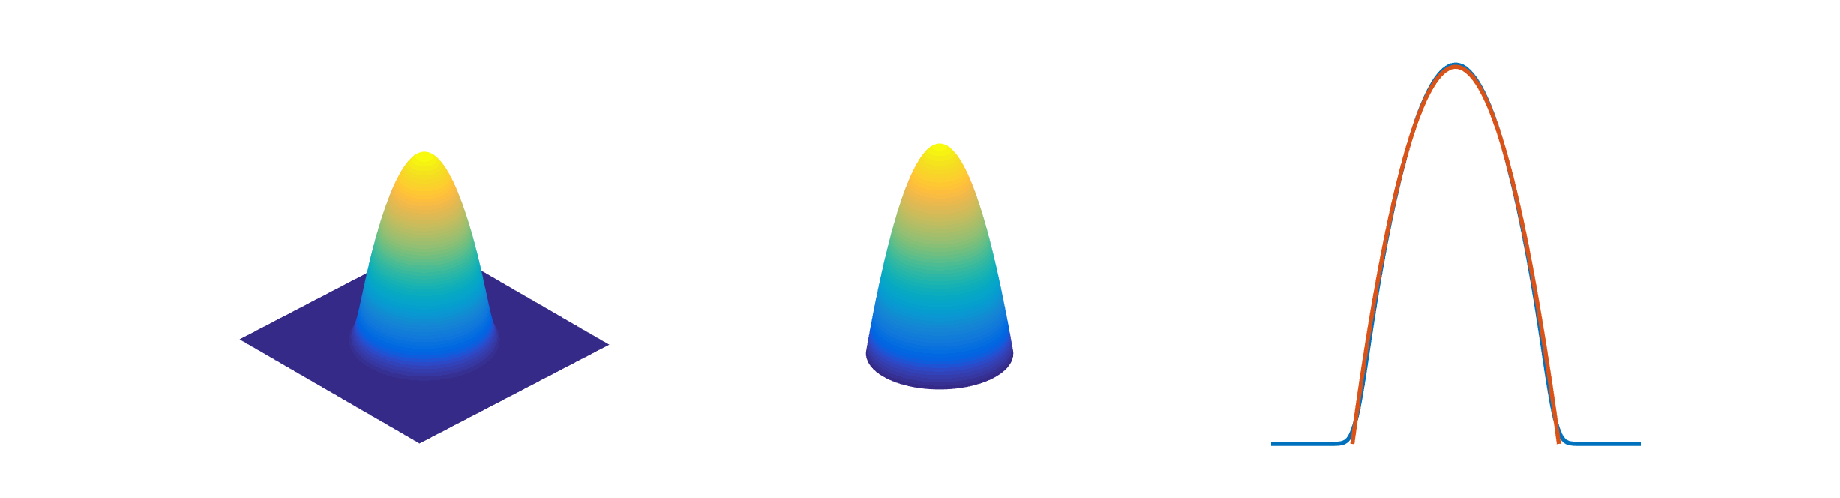
\includegraphics[width=\textwidth,trim=0ex 0ex 0ex 0ex]{Images/ch4_vtx/gpe_tf_3.pdf}
    \caption{The numerical solution (left) and Thomas-Fermi (middle) solutions for a two-dimensional condensate of $^{87}$Rb with $N=1\times 10^5$ atoms. The lineplot (right) is a central cut through both profiles showing the close match.}\label{fig:gpe_tf_3}
\end{figure}

While the Thomas--Fermi solution closely agrees with the numerical solution of the Gross--Pitaevskii equation, this solution is only applicable for stationary states with negligible kinetic energy, i.e.~when the nonlinear interaction dominates over the kinetic energy term. For more complex problems involving dynamics, full numerical integration of the Gross--Pitaevskii equation is required.

One example where the TF approach fails is when investigating superfluid vortex dynamics. To generate vortices in the condensate angular momentum must be added to the system. Seeding a single vortex in the condensate requires that the frequency of rotation, $\Omega$, must be higher than the critical rotation frequency $\Omega_c$, as discussed in Sec.~\ref{ss:vorticesinbec}, and numerically, this is most easily simulated in the co-rotating frame as given by Eq.~\eqref{eqn:gpe_rotation}. Experimentally, there are many ways to create vortices in a condensate, such as stirring with a blue-detuned laser beam \cite{Vtx:Raman_prl_2001}, carefully inverting the trap bias field potential \cite{VTX:Kawaguchi_pra_2004_2,VTX:Masuda_pra_2016}, or through the use of artificial gauge fields \cite{AO:Dalibard_rmp_2011}, to name but a few. In the next sections we will concentrate on solutions where the vortices are already present in the condensate and have settled into the lowest energy configuration.


%%%%%%%%%%%%%%%%%%%%%%%%%%%%%%%%%%%%%%%%%%%%%%%%%%%%%%%%%%%%
\subsection{Few vortex condensates}\label{sec:fewvtx}
%%%%%%%%%%%%%%%%%%%%%%%%%%%%%%%%%%%%%%%%%%%%%%%%%%%%%%%%%%%%

As discussed in Section~\ref{sec:superfluid}, the study of quantum vortices remains an active area of research. As the condensate kinetic energy scales as $E_k \propto l^2$ (Sec.~\ref{ss:vorticesinbec}), increased angular momentum leads to the appearance of more singly charged vortices rather than one multiply charged vortex. For a single vortex in a rotating condensate the only stationary solution that exists is if the vortex resides at the exact centre of the trapping potential, making the system radially symmetric. For two vortices the radial symmetry of the system is broken, with the two vortices arranging themselves in the most favourable position to minimise the energy of the system, as with all higher vortex states. Placing vortices of the same sign into a condensate will allow them to behave as identically charged particles, and they will repel, and form ordered lattices with increasing vortex numbers (see Fig.~\ref{fig:few_rho}). Similarly, if instead we pair a vortex and an antivortex, they will attract, and remain in constant motion, or disappear altogether in the presence of dissipation.

This stability and dynamical behaviour can be understood by examining the velocity fields of the vortices, as shown in Fig.~\ref{fig:vel_field} for like-signed vortices, and Fig.~\ref{fig:vel_pm} for a vortex-antivortex pair. The velocity fields of the vortices are additive, which for like-signed windings creates regions of zero flow, and for opposite-windings creates large flows between them respectively. From Eq.~\ref{eqn:1_over_r} the velocity field of the irrotational quantum vortex scales as $v \propto \frac{1}{r}$, and hence becomes singular at the vortex centre, giving rise to the large velocities close to the singularity. Fig.~\ref{fig:vel_pm_contour} shows a clearer view of the velocity fields as depicted by Fig.~\ref{fig:vel_field}, where the presence of maxima is easily observed at the cores, with field minima also observed due to the vortex-vortex interactions.

\begin{figure}\centering
    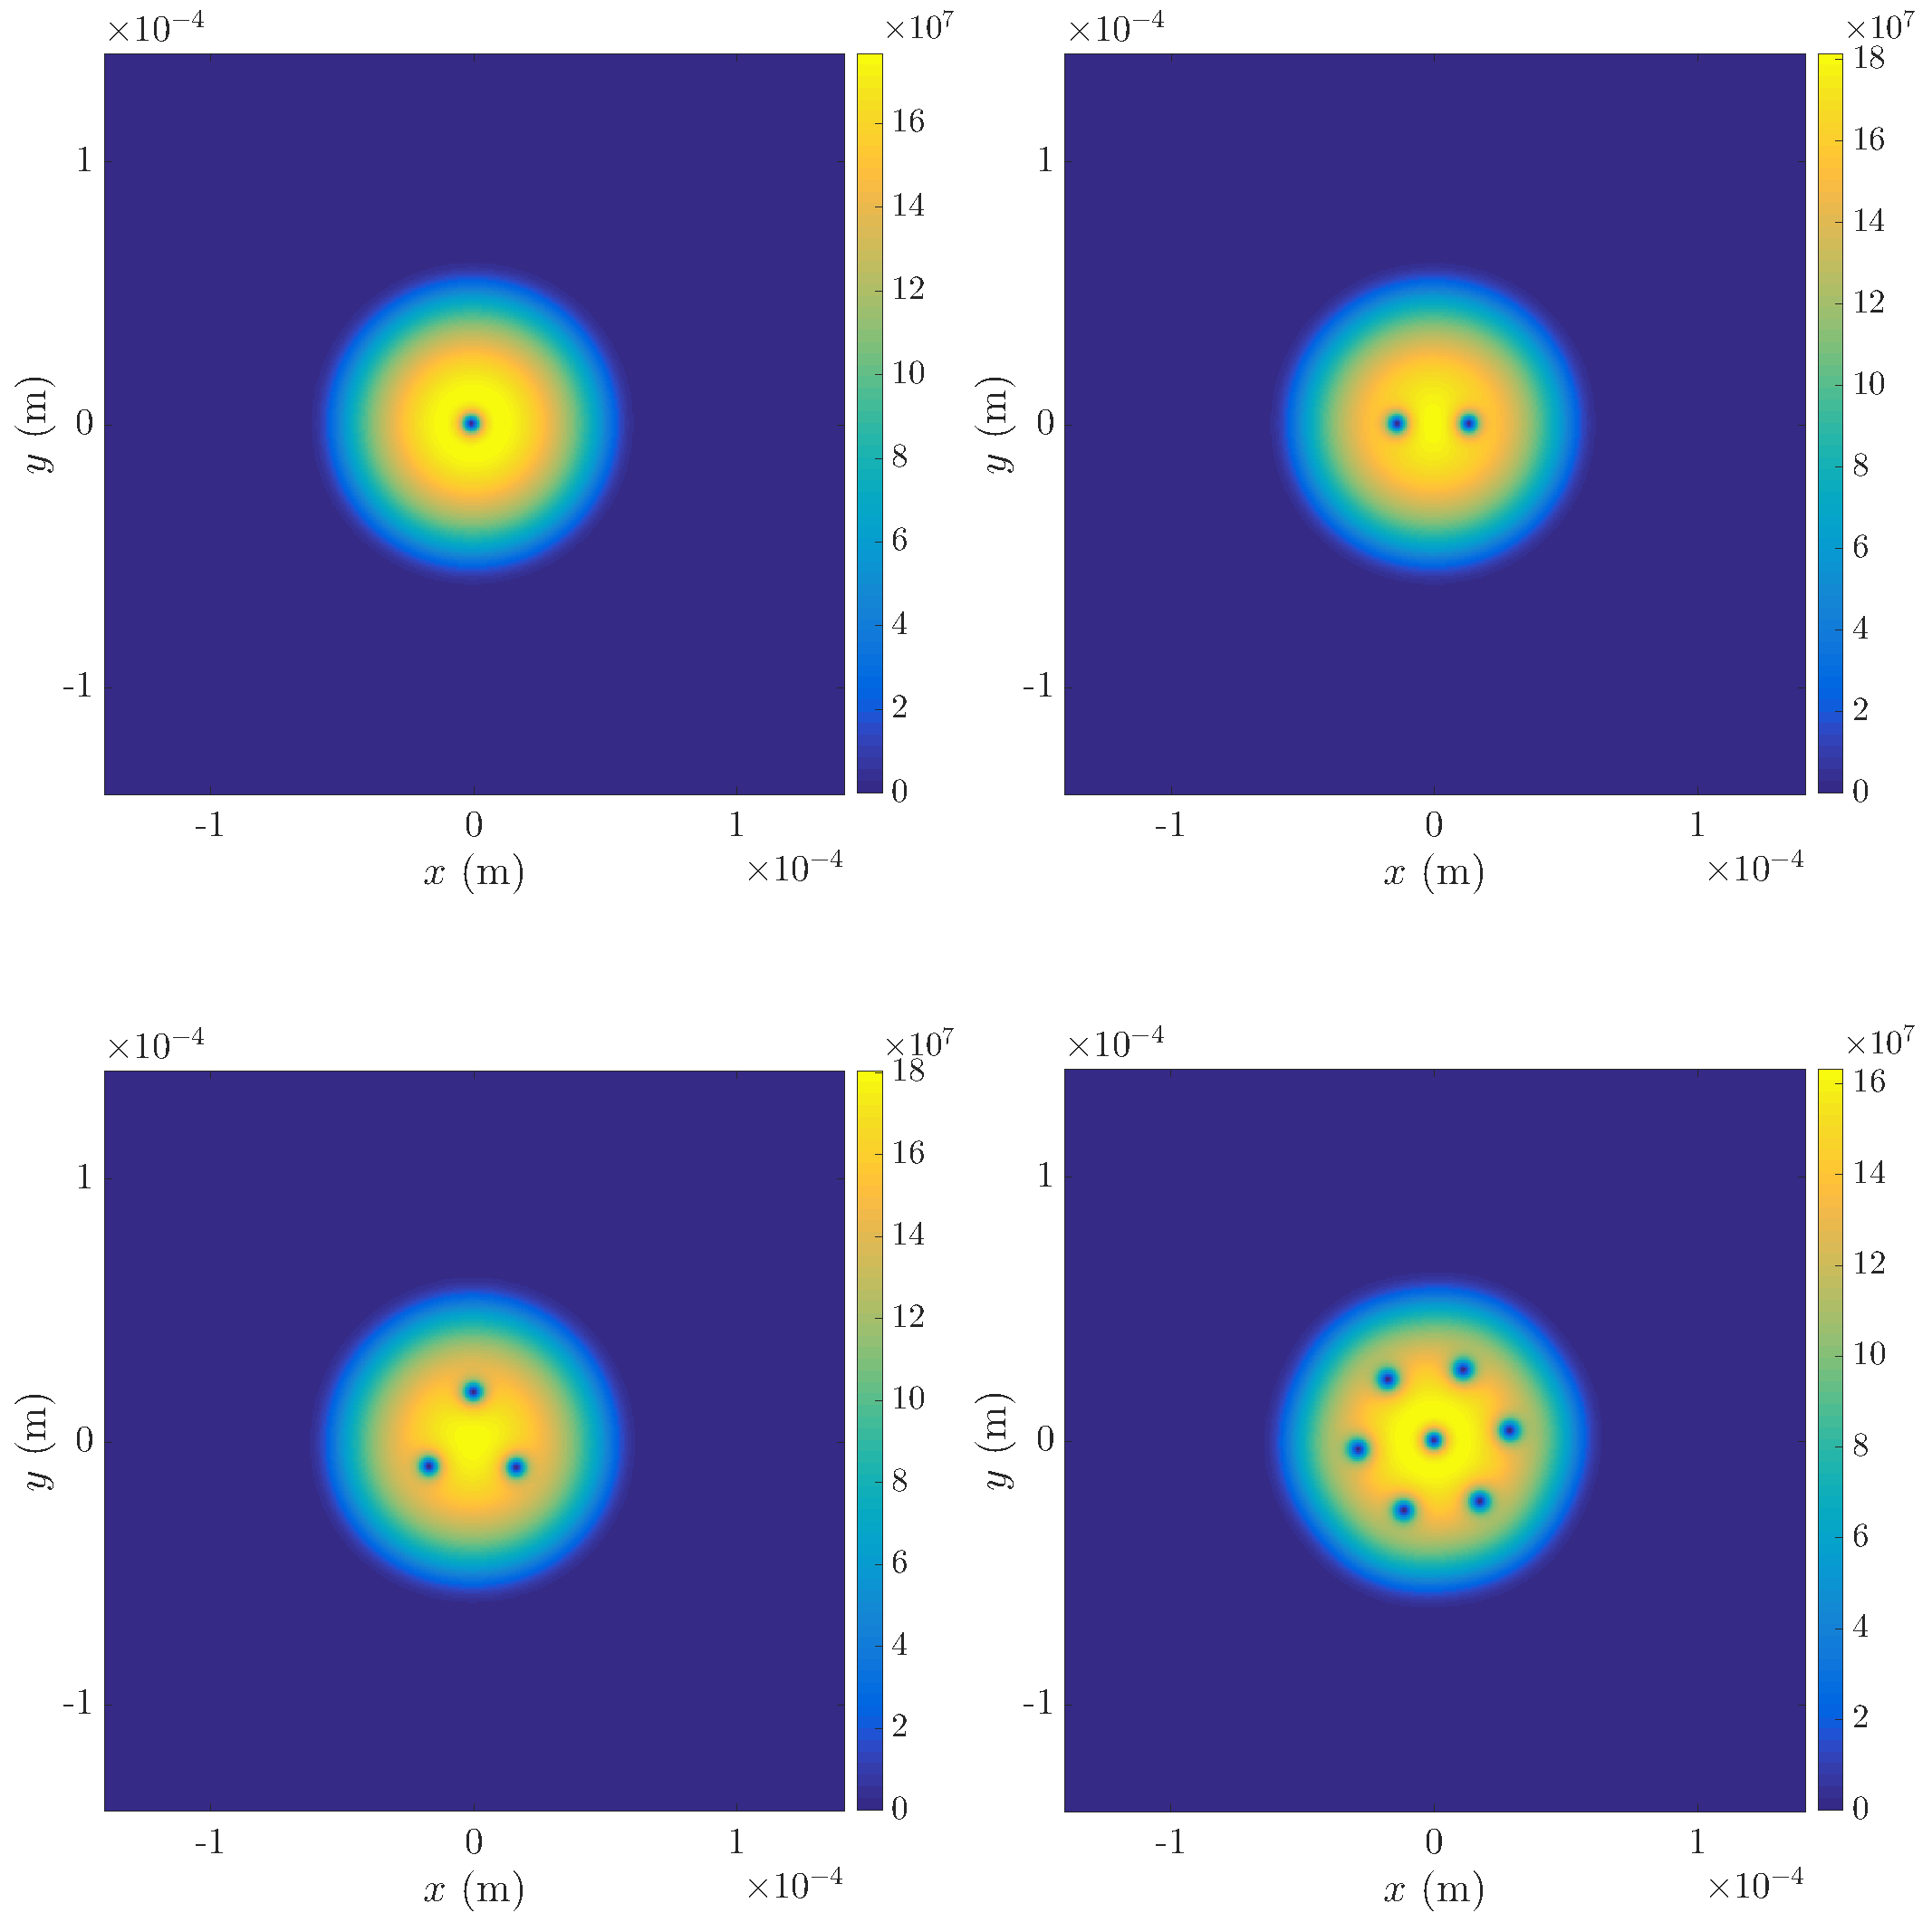
\includegraphics[width=0.48\textwidth]{Images/ch4_vtx/fewvortex_rho.pdf}
    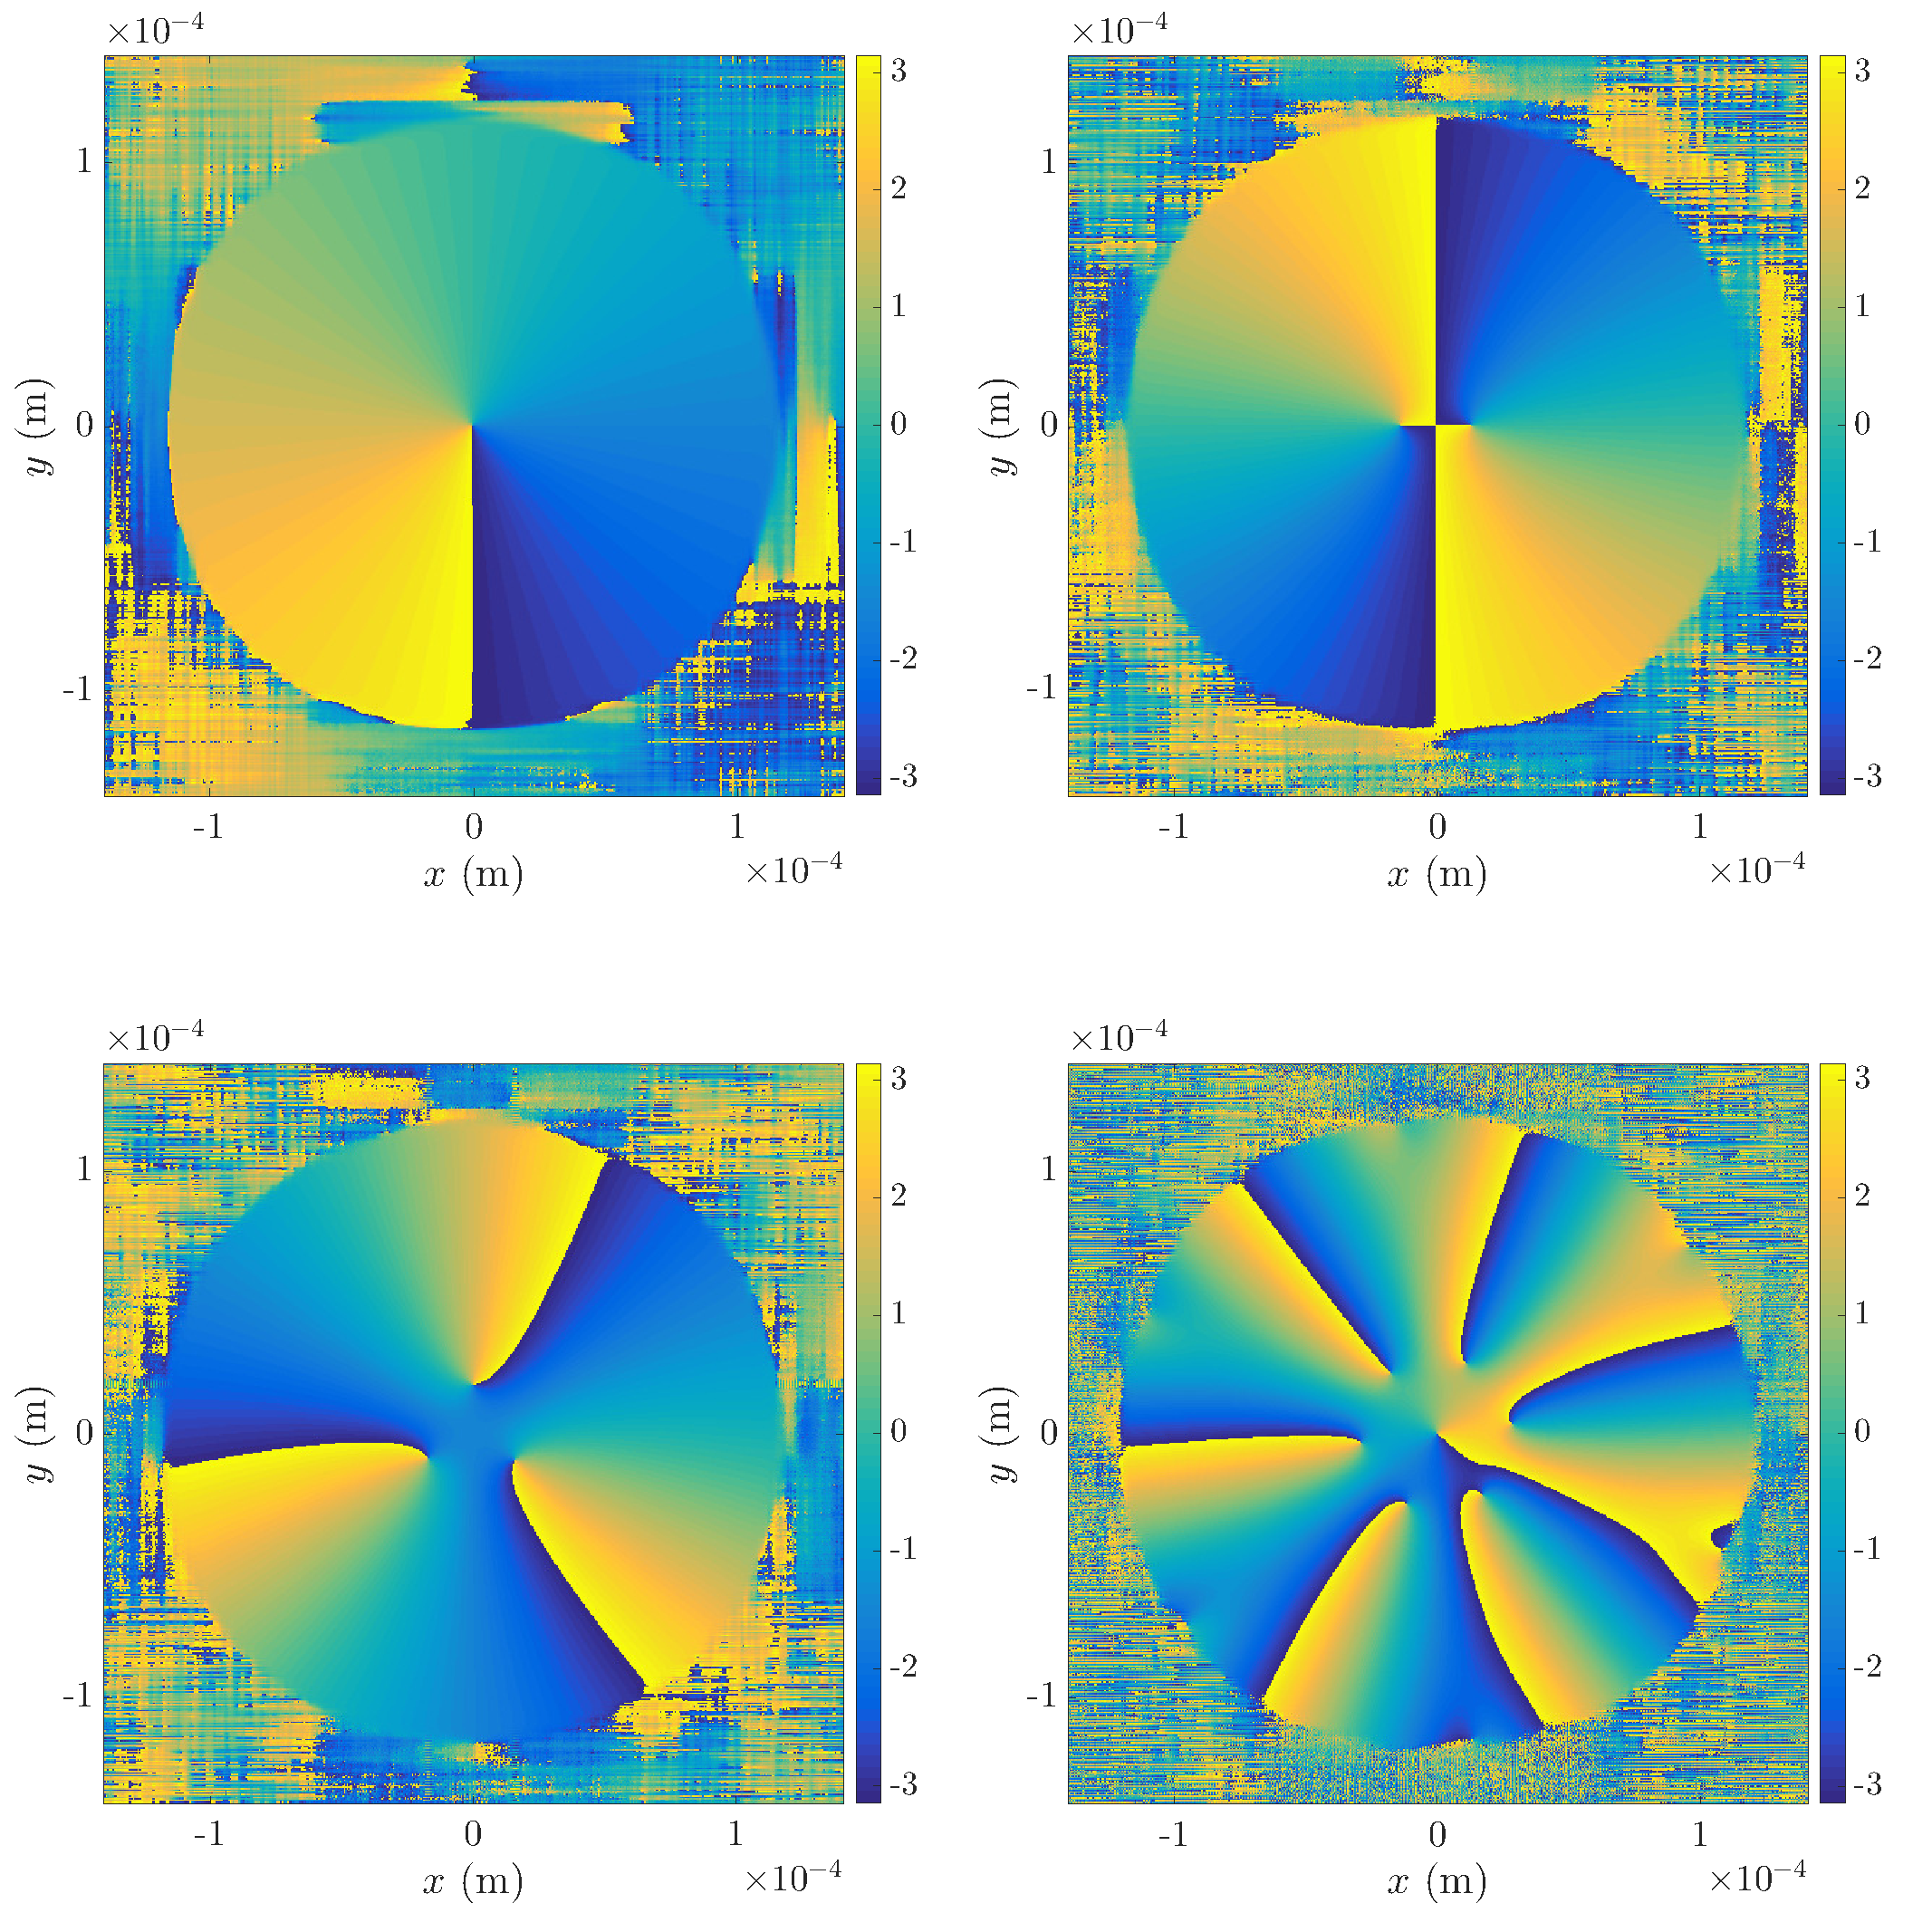
\includegraphics[width=0.48\textwidth]{Images/ch4_vtx/fewvortex_theta.pdf}
    \caption{Density (left) and phase (right) for condensates carrying 1,2,3,and 7 vortices respectively.}
    \label{fig:few_rho}
\end{figure}

\begin{figure}\centering
    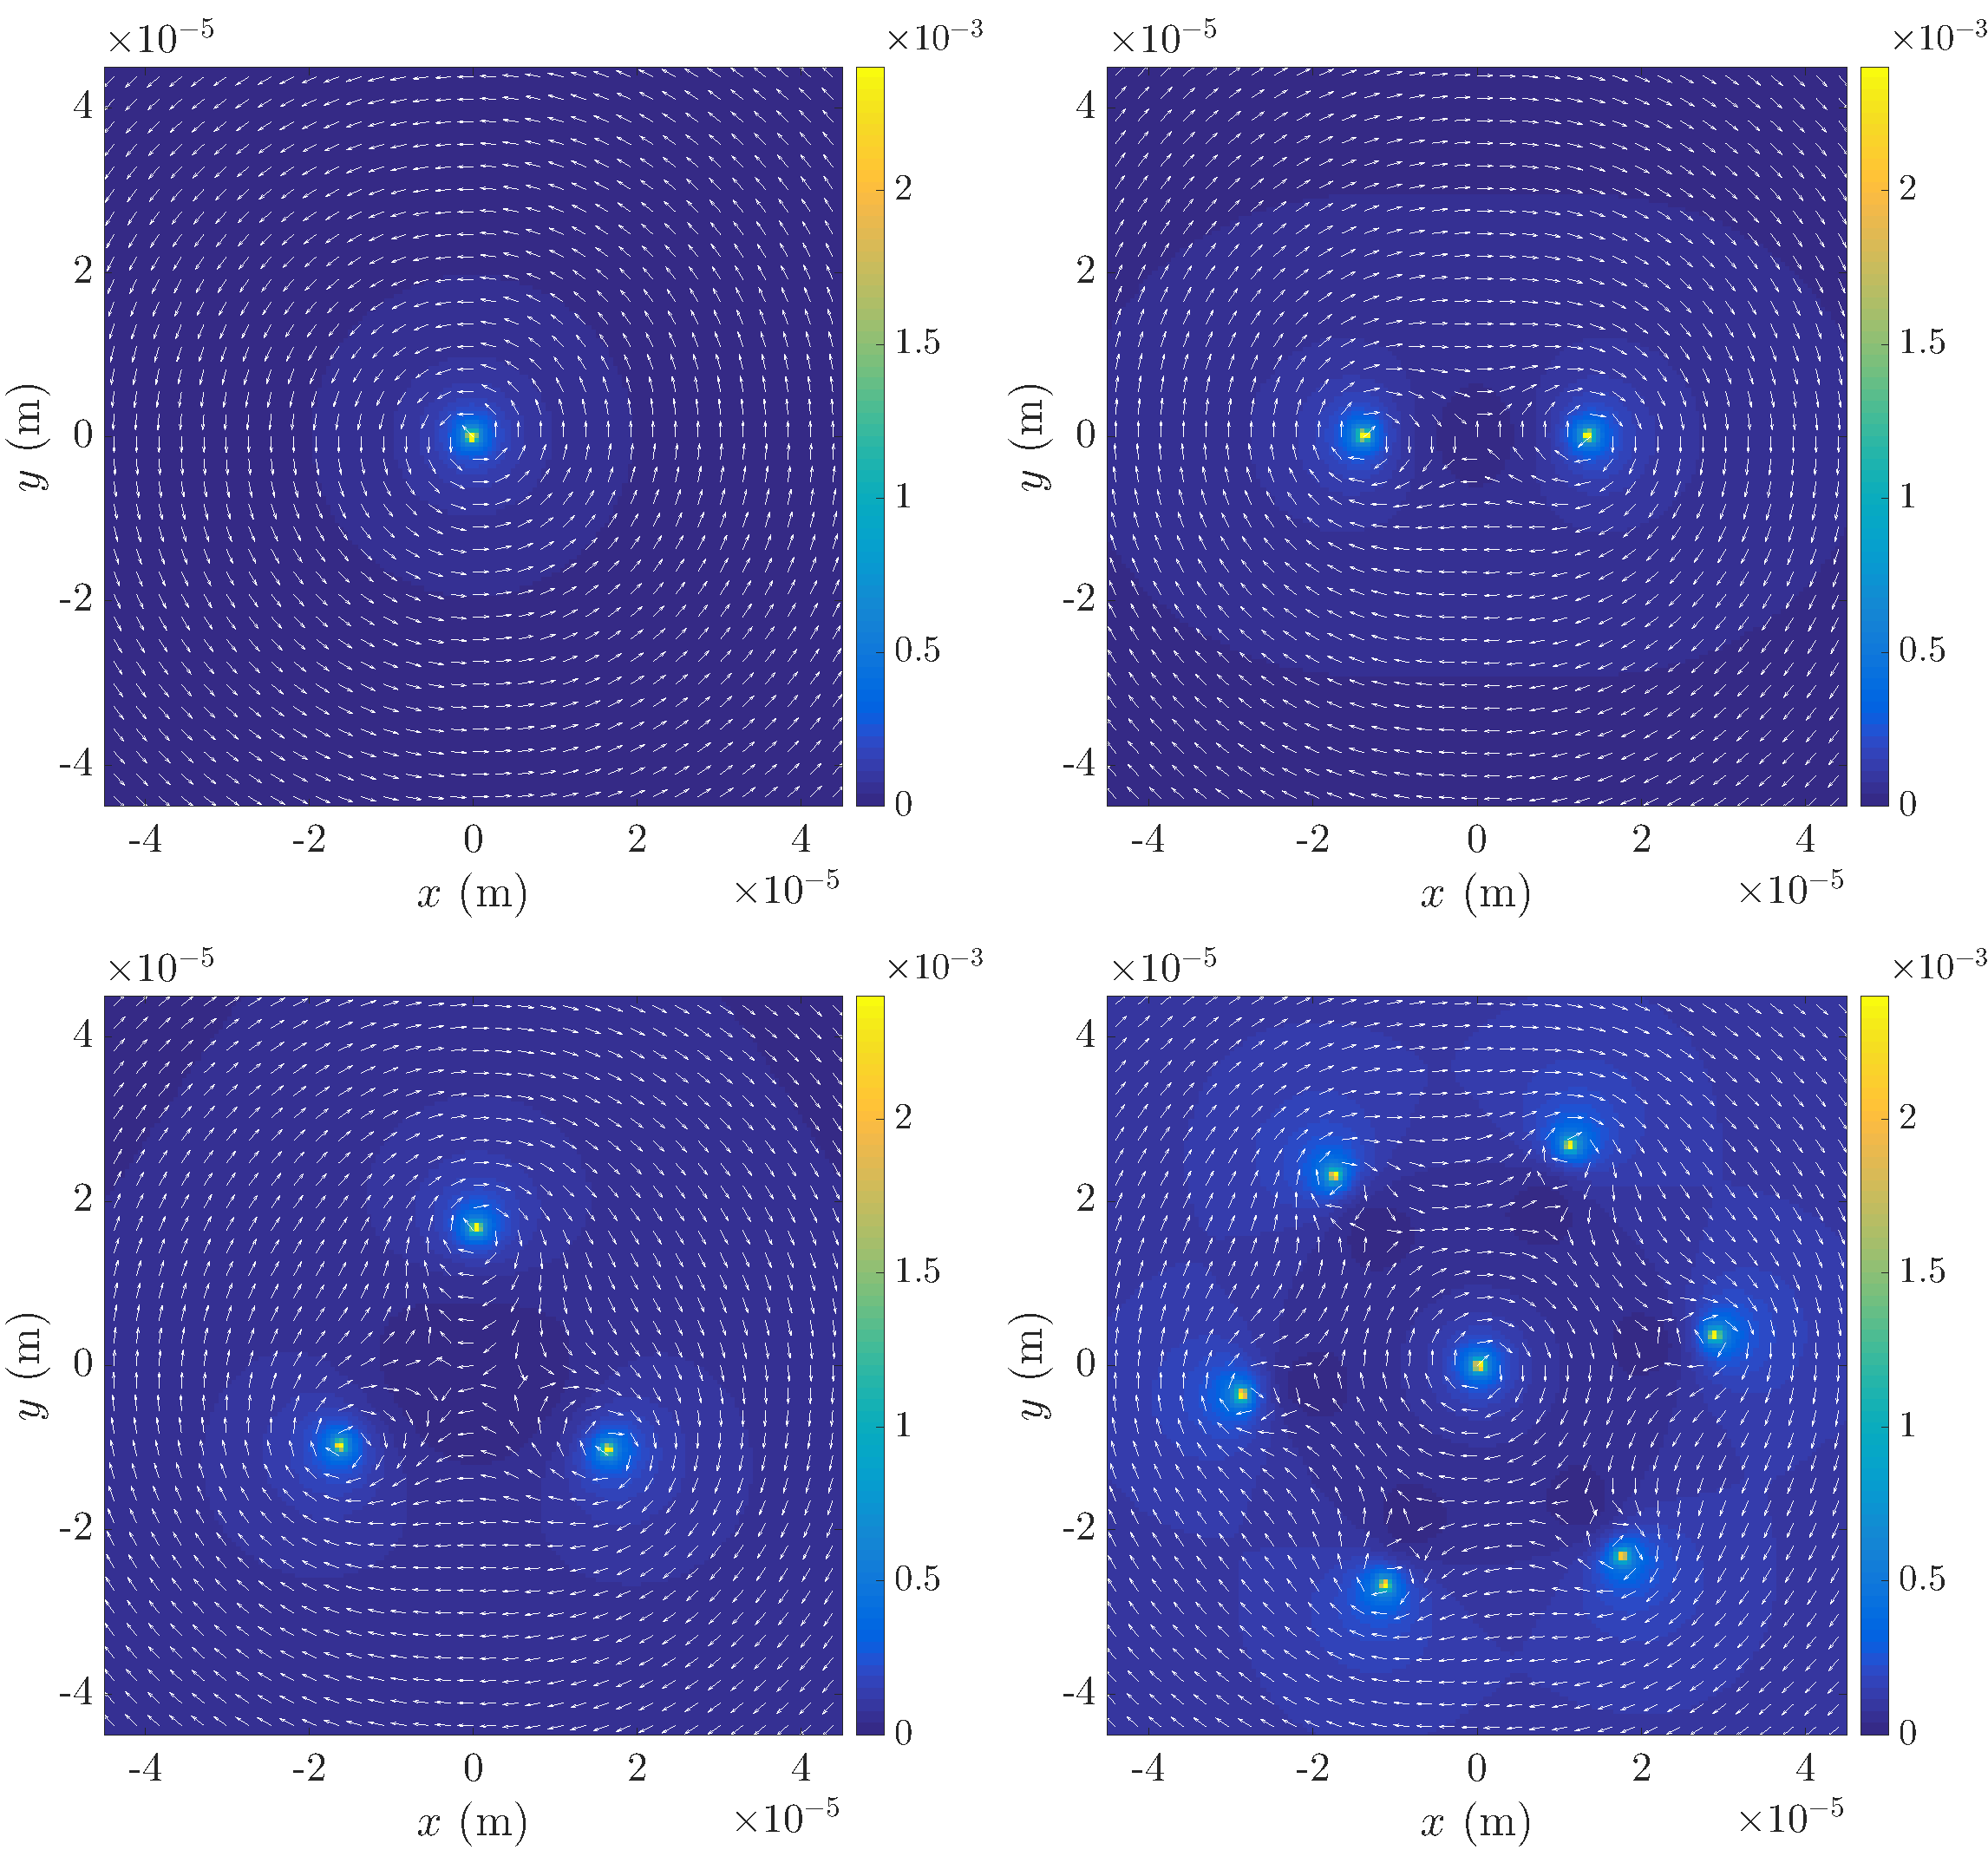
\includegraphics[width=0.95\textwidth]{Images/ch4_vtx/velocity/velocity_fixedmag}
    \caption{Magnitude of the velocity field and the direction of rotation of the field for clockwise circulating vortices. As the velocity follows a $1/r$ profile the magnitude becomes singular at the centre of the vortices, which is capped here at $v=2.4\times 10^{-3}$ (ms$^{-1}$).}
    \label{fig:vel_field}
\end{figure}

\begin{figure}\centering
    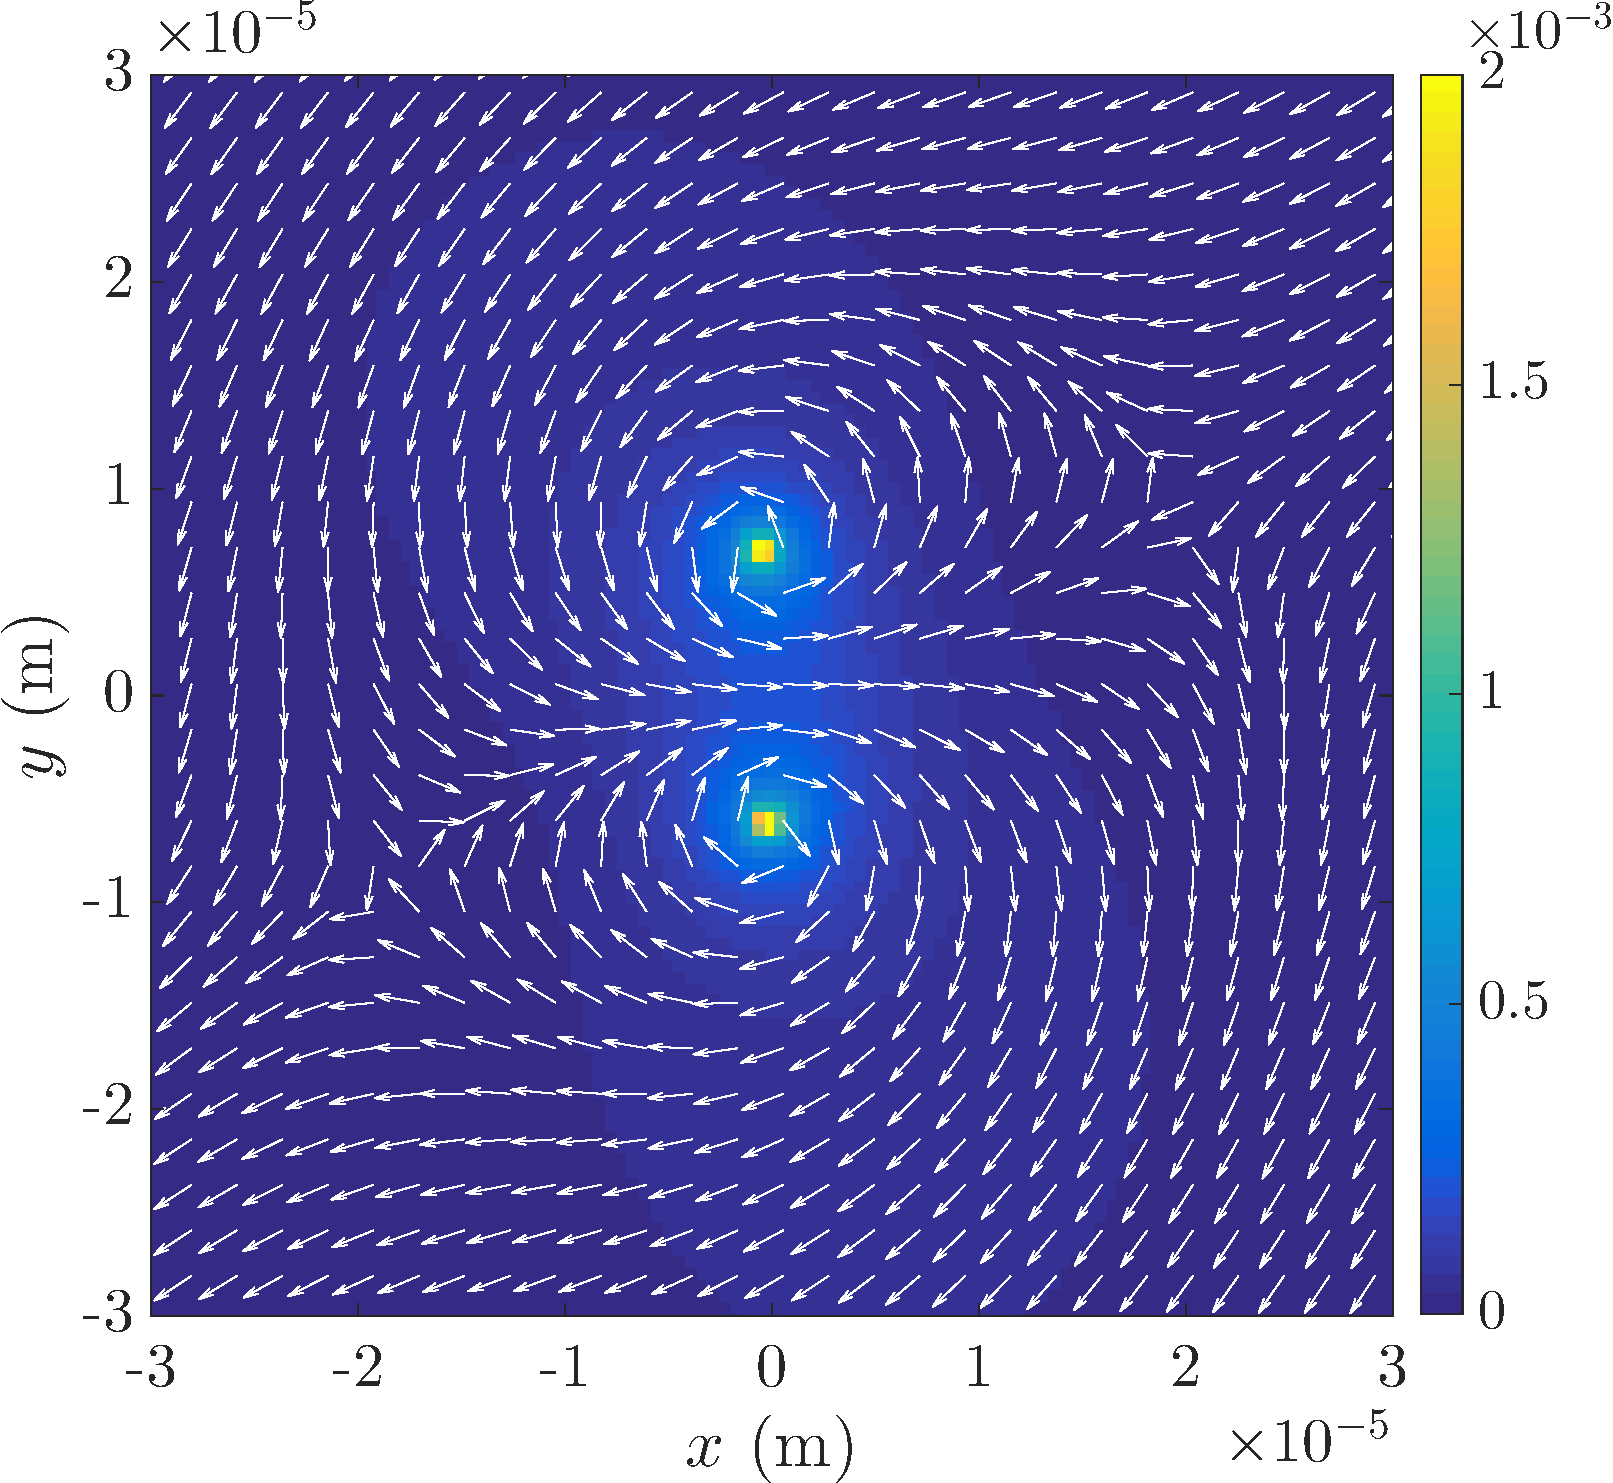
\includegraphics[width=0.55\textwidth]{Images/ch4_vtx/vtx_anti_velfield}
    \caption{Velocity field direction and magnitude originating from vortex and antivortex present in a condensate. Colour scale is in units of ($ms^{-1}$).}
    \label{fig:vel_pm}
\end{figure}

\iffalse
\begin{figure}\centering
    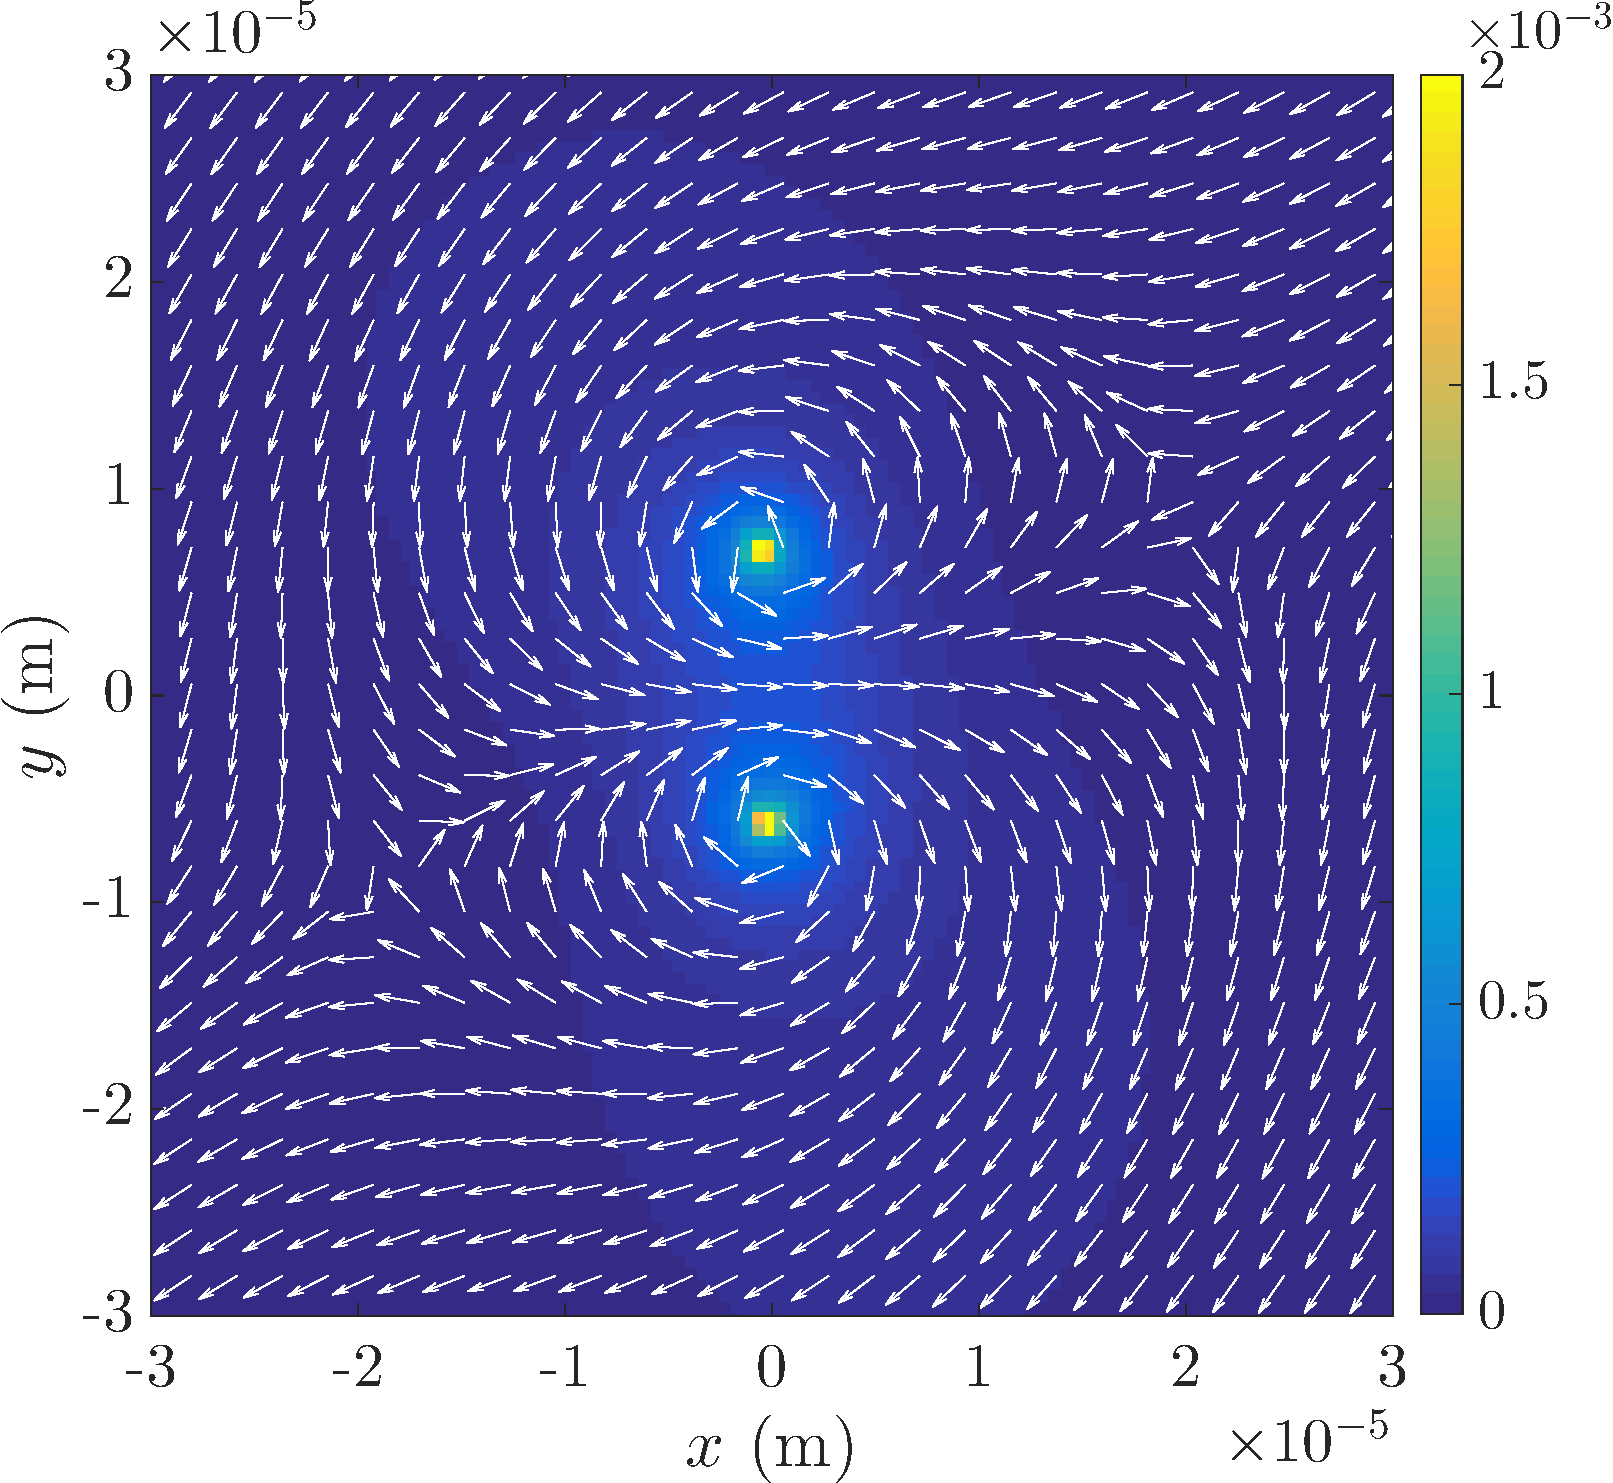
\includegraphics[width=0.45\textwidth]{Images/ch4_vtx/vtx_anti_velfield}
    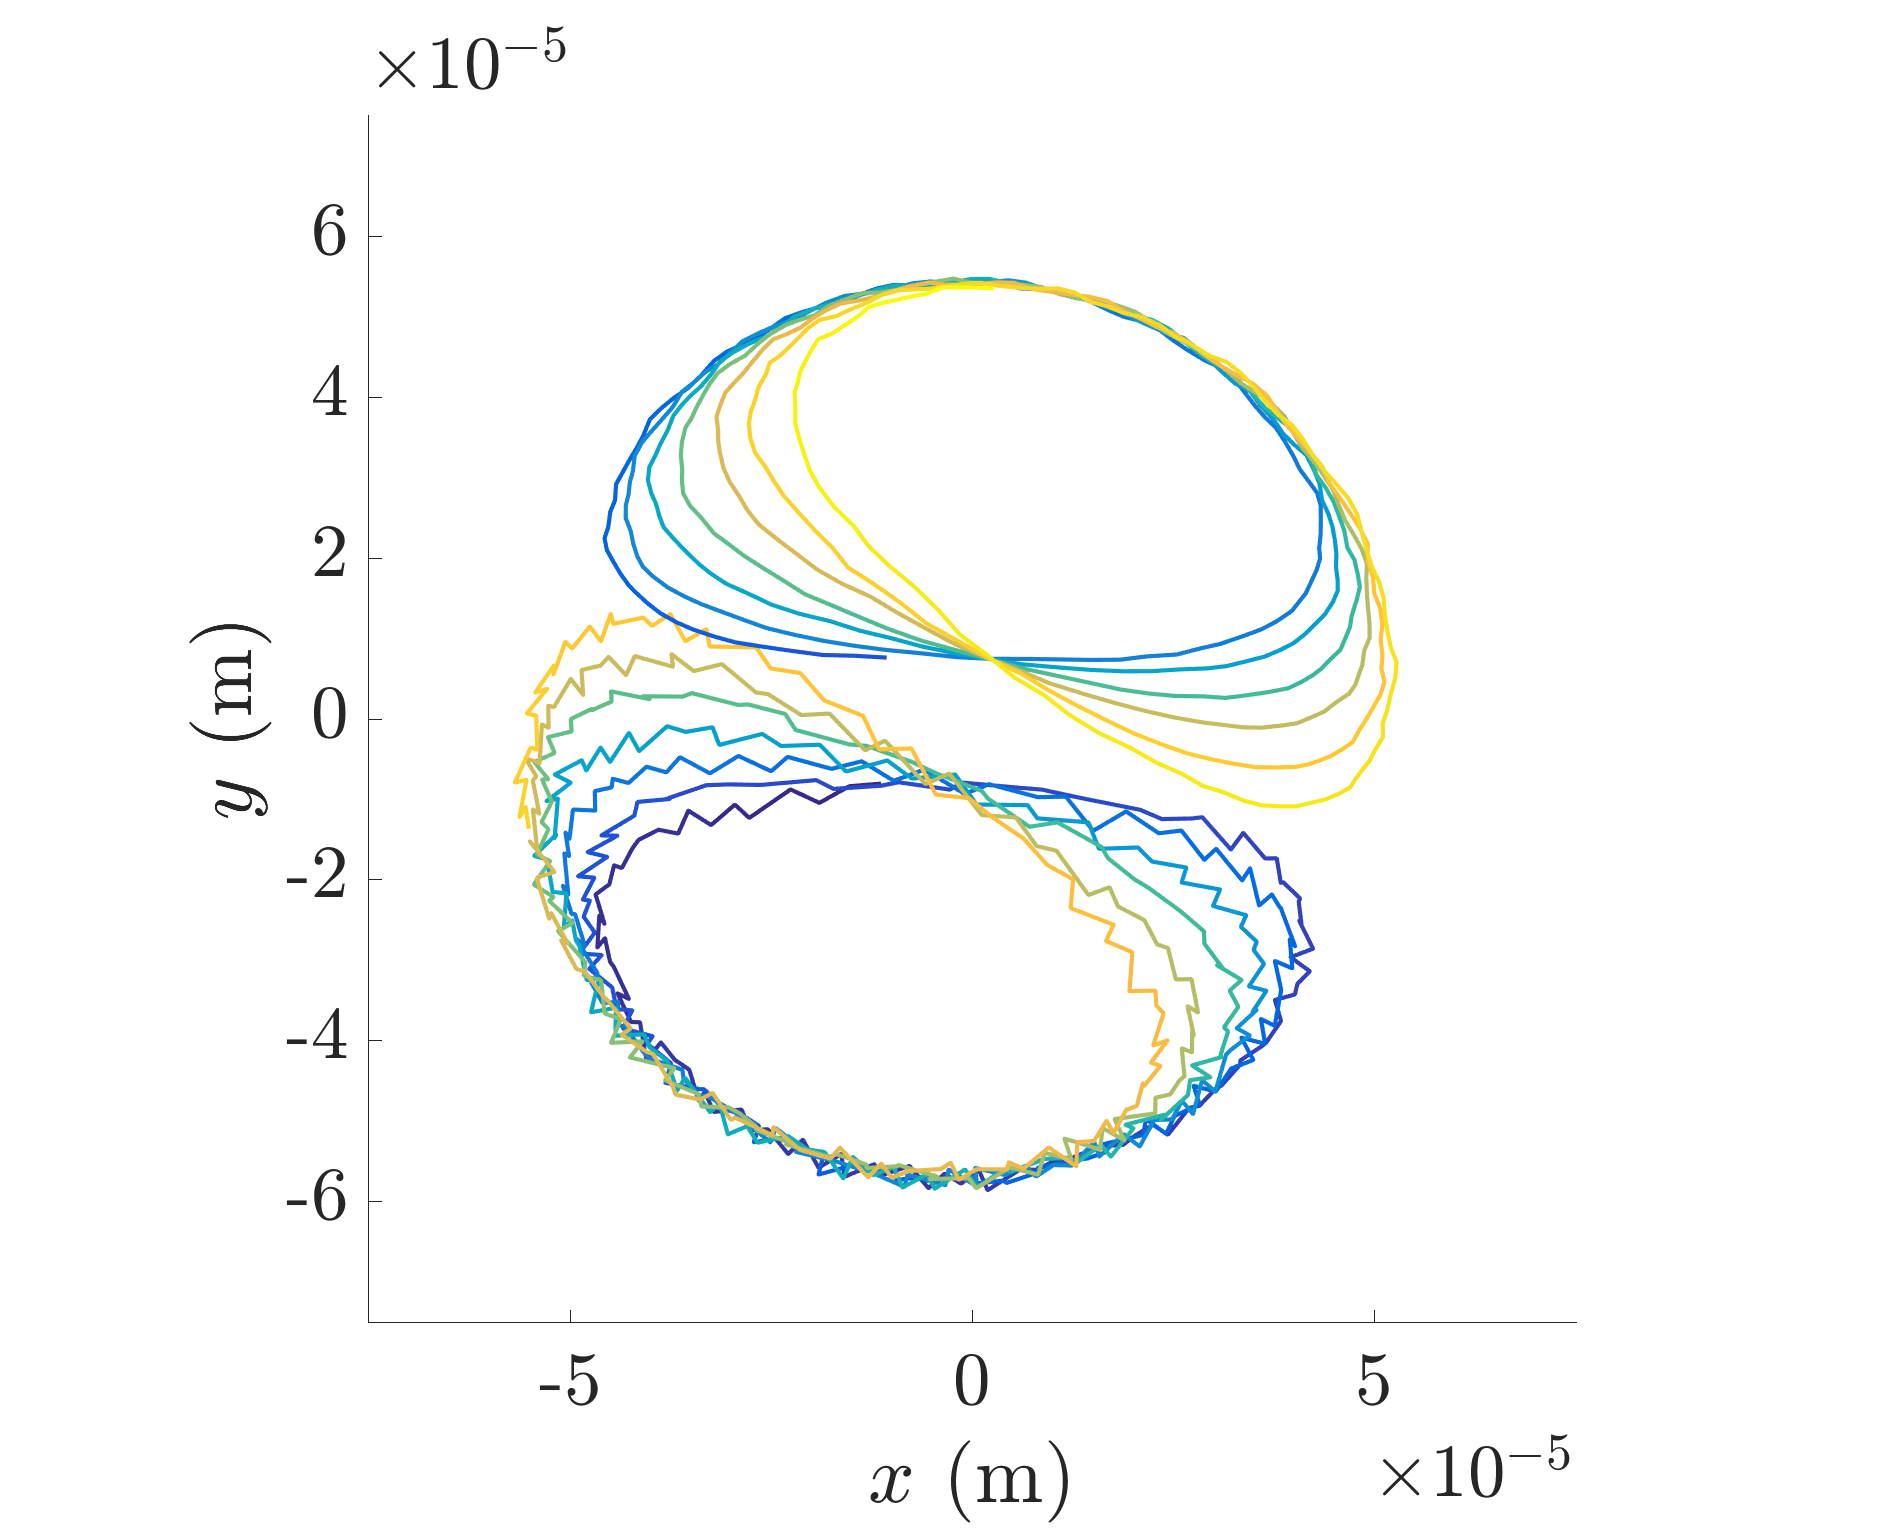
\includegraphics[width=0.45\textwidth]{Images/ch4_vtx/vtx_antivtx_traj}
    \caption{(Left) Velocity field originating from vortex and antivortex present in a condensate. (Right) Trajectories of vortex and antivortex in a condensate in the lab frame. Vortices travel on circulating paths which will always intersect through their starting position. Color is used to represent the same times for both vortex and antivortex, which is on the order of seconds.}
    \label{fig:vel_pm}
\end{figure}
\fi

\begin{figure}\centering
    %\includegraphics[width=0.95\textwidth]{Images/ch4_vtx/velocity/vel_axis_png}
    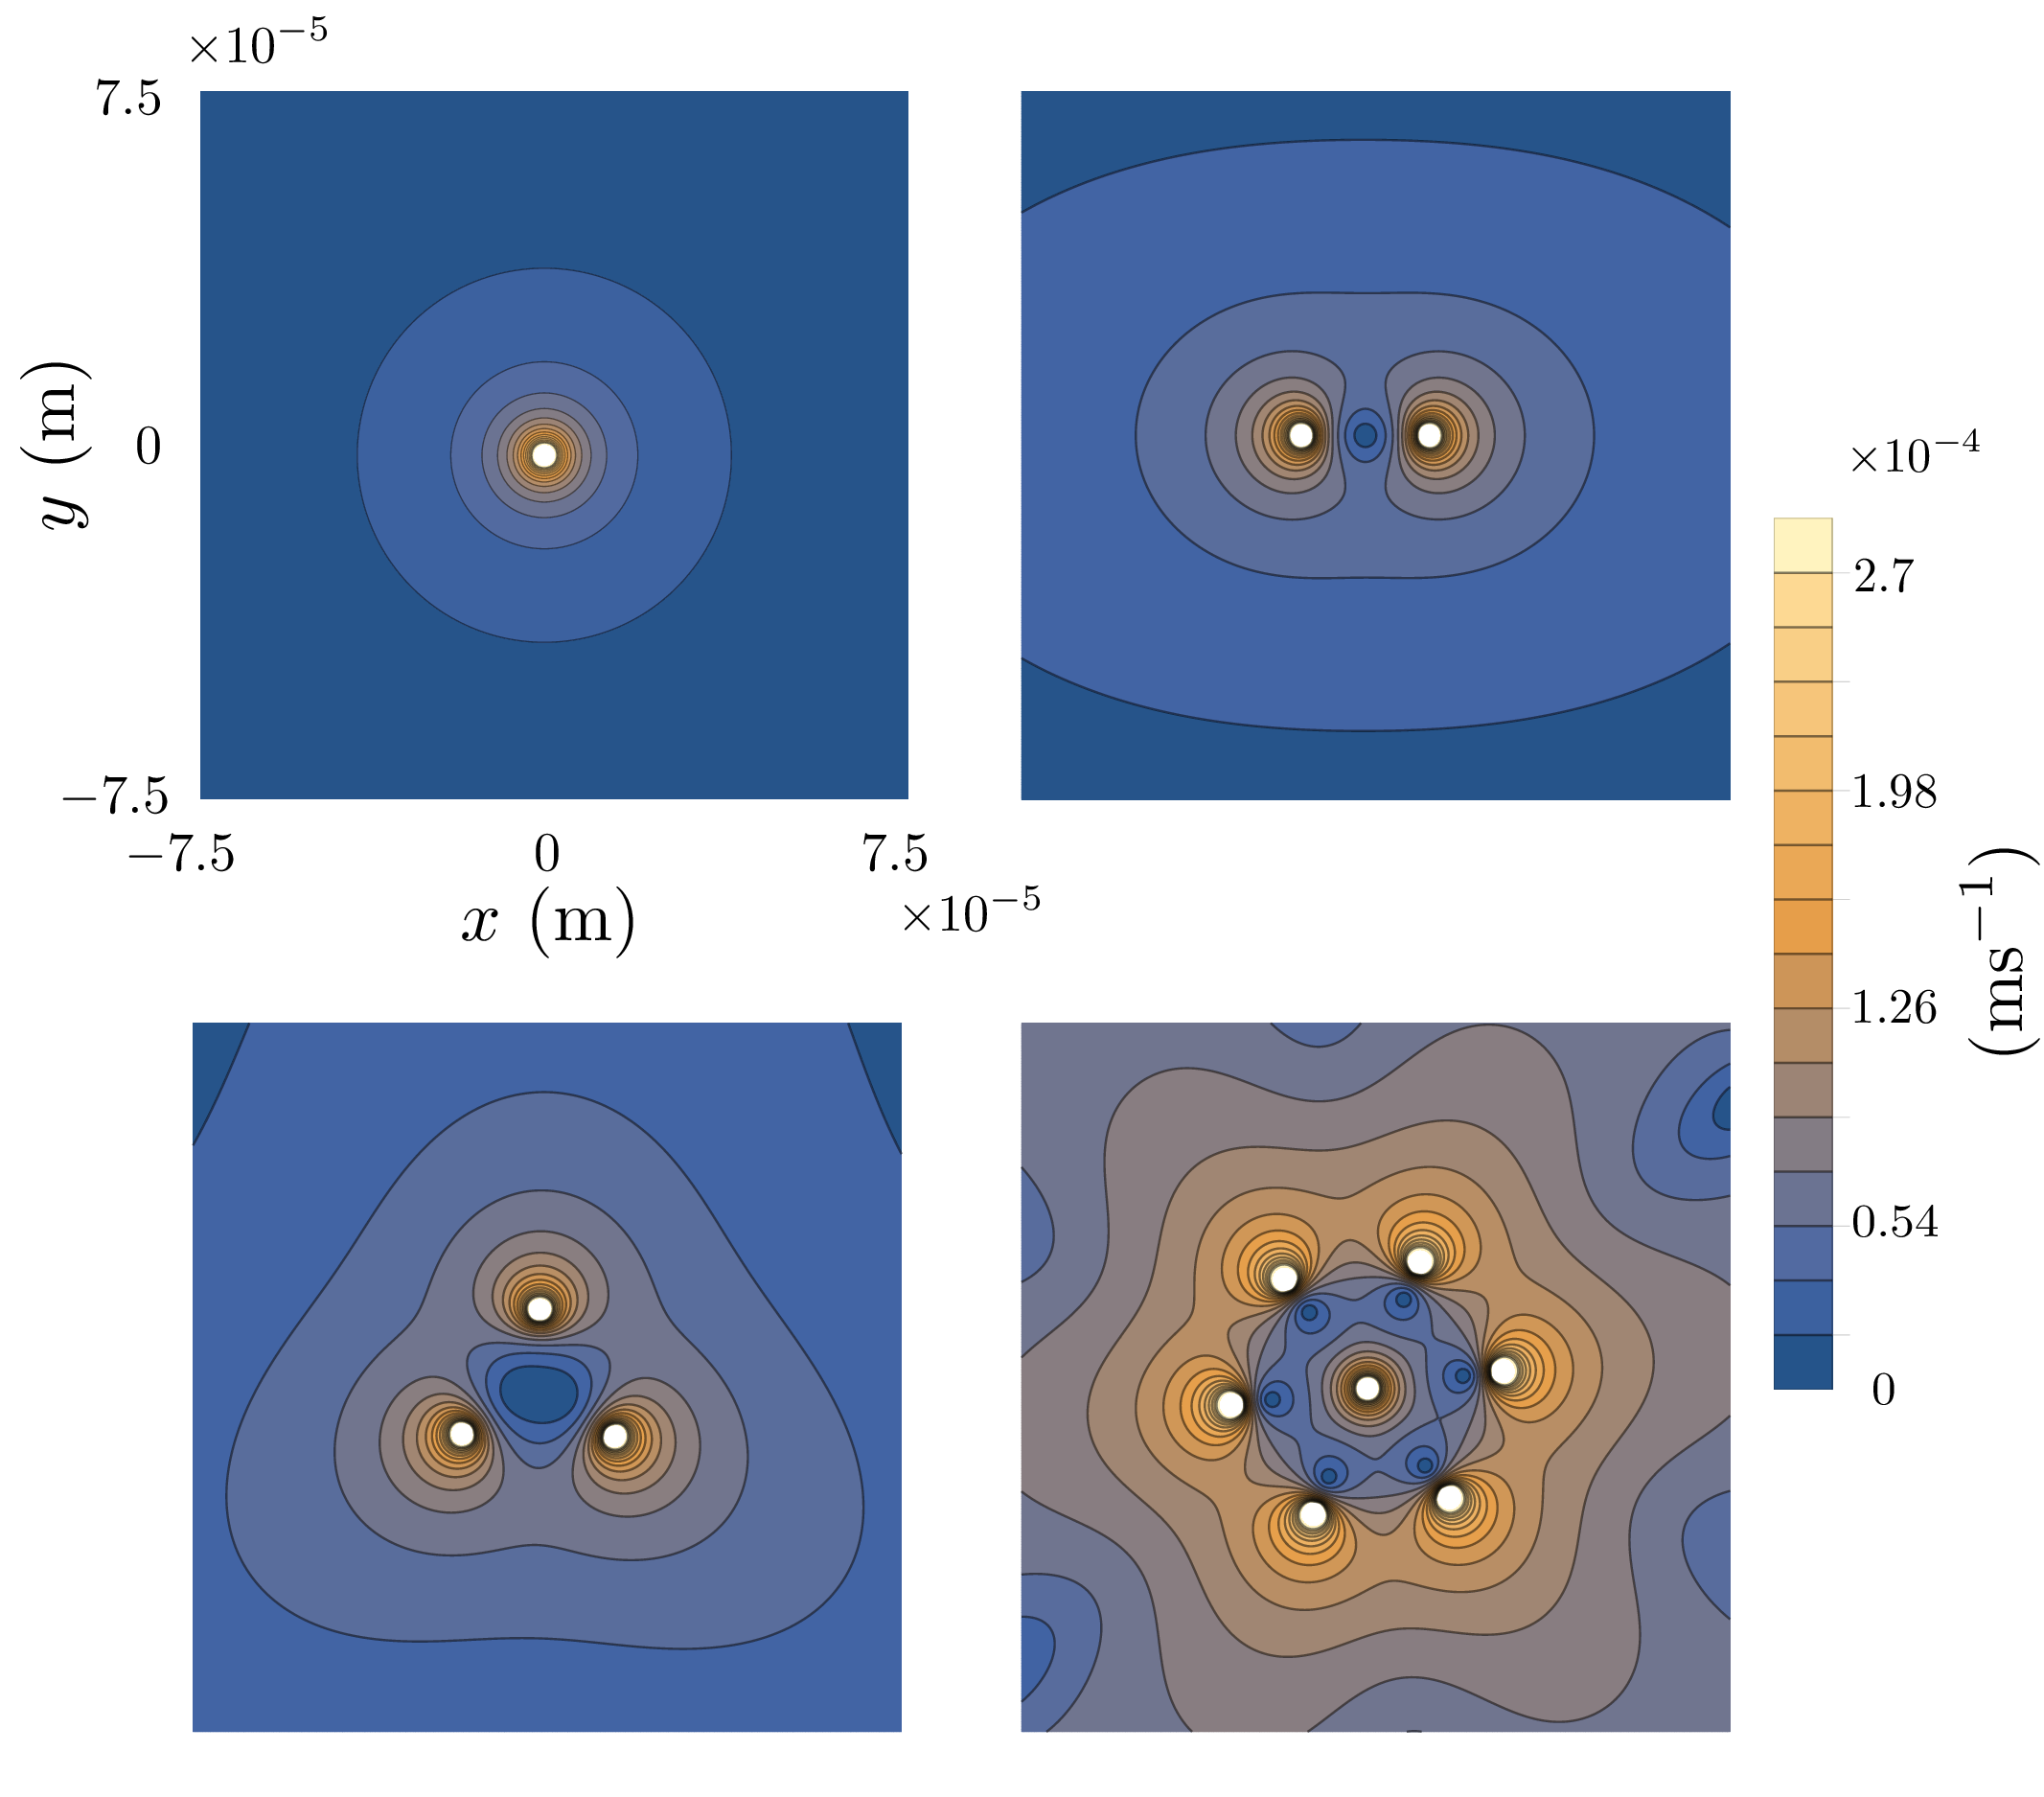
\includegraphics[width=0.95\textwidth]{Images/ch4_vtx/velocity/vel.png}
    \caption{Magnitude of the velocity field for small numbers of like-signed vortices in a condensate. The velocity field can be seen to become singular at the centre, which here has its magnitude capped at a lower value than Figs.~\ref{fig:vel_field} and~\ref{fig:vel_pm} to aid visibility. Regions of minimal velocity are seen, wherein the opposing field lines compensate one another.}
    \label{fig:vel_pm_contour}
\end{figure}


%%%%%%%%%%%%%%%%%%%%%%%%%%%%%%%%%%%%%%%%%%%%%%%%%%%%%%%%%%%%
\section{Rapidly rotating vortex lattice}
%%%%%%%%%%%%%%%%%%%%%%%%%%%%%%%%%%%%%%%%%%%%%%%%%%%%%%%%%%%%

%%%%%%%%%%%%%%%%%%%%%%%%%%%%%%%%%%%%%%%%%%%%%%%%%%%%%%%%%%%%
\subsection{Model system}\label{sec:modelsystem}
%%%%%%%%%%%%%%%%%%%%%%%%%%%%%%%%%%%%%%%%%%%%%%%%%%%%%%%%%%%%
%\todo[inline]{Fix velocity fields of all the plots and ensure they are all using the same units and similar ranges.}
%\todo[inline]{Explain away the antivortex wobble}
For the work to follow we assume a standard single component Bose--Einstein condensate in a radially symmetric trap of frequency $\omega_\perp = 2\pi \times 1$ Hz. By tightly confining the condensate along the $z$-dimension, with trapping frequency $\omega_z = 2\pi\times 16$ Hz, such that $\omega_z $ is greater than $ \omega_\perp$, the condensate enters the desired pancake-shaped geometry. The system is then modelled using the mean-field GPE Hamiltonian as
\begin{equation}\label{eqn:gpe_h0}
	H_{\mathrm{GP}} = -\frac{\hbar^2}{2m}\nabla^2 + \frac{1}{2}m\omega_{\perp}^2\mathbf{r}^2 + g_{2D}\vert\Psi(\mathbf{r},t)\vert^2.
\end{equation}

Here, we define the two-dimensional effective interaction strength $g_{2D}$ given by Eq.~\eqref{eqn:g2d_efint}, as
\begin{equation}
g_{2D} = g\sqrt{\frac{m\omega_z}{2\pi\hbar}} = 4g \sqrt{\frac{m}{\hbar}}.
\end{equation}

To describe the system we enter the co-rotating frame, which is done by including the angular momentum operator $L_z$ in the Hamiltonian. The time dependent dynamics of the system are then given by the GPE as
\begin{equation}\label{eqn:gpe2d_}
	i\hbar\partial_t\Psi(\mathbf{r},t) = \left[ H_{\text{GP}}  -  \Omega L_z \right] \Psi(\mathbf{r},t).
\end{equation}

If the angular rotation frequency approaches the condensate trapping frequency, $\Omega_z \approx \omega_\perp$, the condensate gains a large triangular lattice of vortices.  The effect of setting $\Omega_z=\omega_\perp$, can be partially understood in a mean-field setting by rewriting the GPE kinetic and rotation terms in the form
\begin{equation}
    \frac{\mathbf{p}^2}{2m} + \frac{m\Omega\mathbf{r}^2}{2} - \Omega L_z = \frac{\mathbf{\left(p -m\boldsymbol{\Omega}\times\mathbf{r}\right)^2}}{2m}.
\end{equation}

The resulting changes to the GPE are then given by
\begin{equation}\label{eqn:vector_potential_gpe}
    \textrm{i}\hbar\partial_t \Psi =
    \left(\frac{1}{2m}(-i\hbar\nabla - m\boldsymbol{\Omega}\times\mathbf{r})^2 + \frac{m}{2}(\omega_\perp - \Omega)^2{r}^2 + g_{2D}|\Psi|^2 \right)\Psi.
\end{equation}
The above Hamiltonian demonstrates the correspondence between a rotating condensate and that of a non-relativistic charged particle in a magnetic field~\cite{Vtx:Mueller_prl_2002}.
%\begin{equation}
%     H_L = \frac{1}{2m}\left(-i\hbar \nabla  - q\mathbf{A}\right)^2 + q\phi
%\end{equation}
%where $q$ is the particle charge, $\mathbf{A}$ is the respective gauge potential, and $\phi$ the respective scalar potential.
One can see that when the rotation and trapping frequencies are equal, the condensate no longer sees a confining potential, due to the centrifugal force experienced, given by the term $-m\Omega_z^2r^2/2$.

As stated earlier in Sec.~\ref{sec:sec2_vtxlatt} as $\Omega_z$ approaches $\omega_\perp$, the use of mean-field theory becomes less justified, and the system enters a strongly correlated regime. If the filling fraction $\nu$ is in the range of $10 \leq \nu \leq 1000$, the system enters the ``mean-field quantum Hall'' regime, where the Gross--Pitaevskii theory is still working well. The regime exists up to an upper limit frequency of $\Omega_z = 0.995\omega_\perp$, so that we can work with systems that have a very large vortex lattice, and are still described by mean-field theory \cite{BEC:Fetter_revmodphys_2009}.

In the following we will numerically solve Eq.~\eqref{eqn:gpe2d_}, using the pseudospectral Fourier split operator method and making use of GPU computing as described in Sec.~\ref{sec:GPUE}. For realistic experimental parameters we assume  $N\approx 10^6$ atoms of $^{87}$Rb, with an $s$-wave scattering length of $a_s=4.76\times10^{-9}$ m~\cite{AO:Roberts_prl_1998}. The numerically evaluated ground-state for the given set of parameters is shown previously in Fig.~\ref{fig:showingoff} and has a radius of approximately $3.5\times 10^{-4}$ m. For these parameters, the number of vortices within the visible density region is approximately 600, giving a filling factor of $\nu \approx 800 $. This places the system within the mean-field quantum Hall regime, and therefore a description using Gross--Pitaevskii theory is adequate~\cite{Vtx:Schweikhard_prl_2004}.

Following an imaginary time-evolution as outlined in Sec.~\ref{sec:timeev}, we first find the groundstate of the condensate in a harmonic potential, starting with a condensate without vortices. We then linearly ramp the rotation frequency to avoid the lattice disordering issue discussed in Sec.~\ref{ss:ang_mom_fso}. This allows us to follow the groundstate solution at all times while the rotation frequency is increased, which has the added advantage of returning a groundstate solution for any required rotation frequency. Examples of several states obtained during a single simulation are given in Fig.~\ref{fig:inc_omega}. The previously discussed resolution considerations become apparent as the rotation rate is increased for both the position and momentum space representations of the wavefunction. A movie of the wavefunction density is available at the following URL~\cite{YT:BEC_gen}, in which the frequency is ramped from $\Omega/\omega_\perp = 0.39 \to 0.995$.

The rapidly rotating vortex lattice is known to exhibit solid-body-like rotation \cite{Vtx:AboShaeer_sci_2001}. This can be seen in Fig.~\ref{fig:solidbody}, where the coarse-grained flow of the velocity field increases as a function of the distance from the lattice centre. This rigid-body behaviour allows us to treat the lattice as a solid object. Recalling the Feynman relation for vortex density Eq.~\eqref{eqn:feynman}, $n_v = m\Omega/(\pi\hbar)$, we choose an area over which the lattice spacing is almost constant and the vortex density closely matches this relation. In this regime the vortices close to the centre will have an almost uniform profile~\cite{VTX:Watanabe_pra_2006}; for the above system parameters this is fulfilled by a hard-walled radial boundary of $r=2\times 10^{-4}$ m, in which the number of vortices are calculated to being $n_v \approx 342$. Employing the vortex detection and tracking methods described in Sec.~\ref{sec:vortrack}, within the same region gives $n_v = 341$ vortices, with a lattice spacing of $a_v \approx 2.1\times 10^{-5}$ m, and with a standard deviation of $\sigma \approx 2.7 \times 10^{-7}$ m. These values indicate that within this region the lattice is well ordered. While the condensate has more vortices outside this boundary that are initially ordered, during time evolution many of these move more easily due to the large velocity fields closer to the edges. The above boundary gives a well ordered lattice that remains well ordered for several seconds of time evolution.

\begin{figure}\centering
    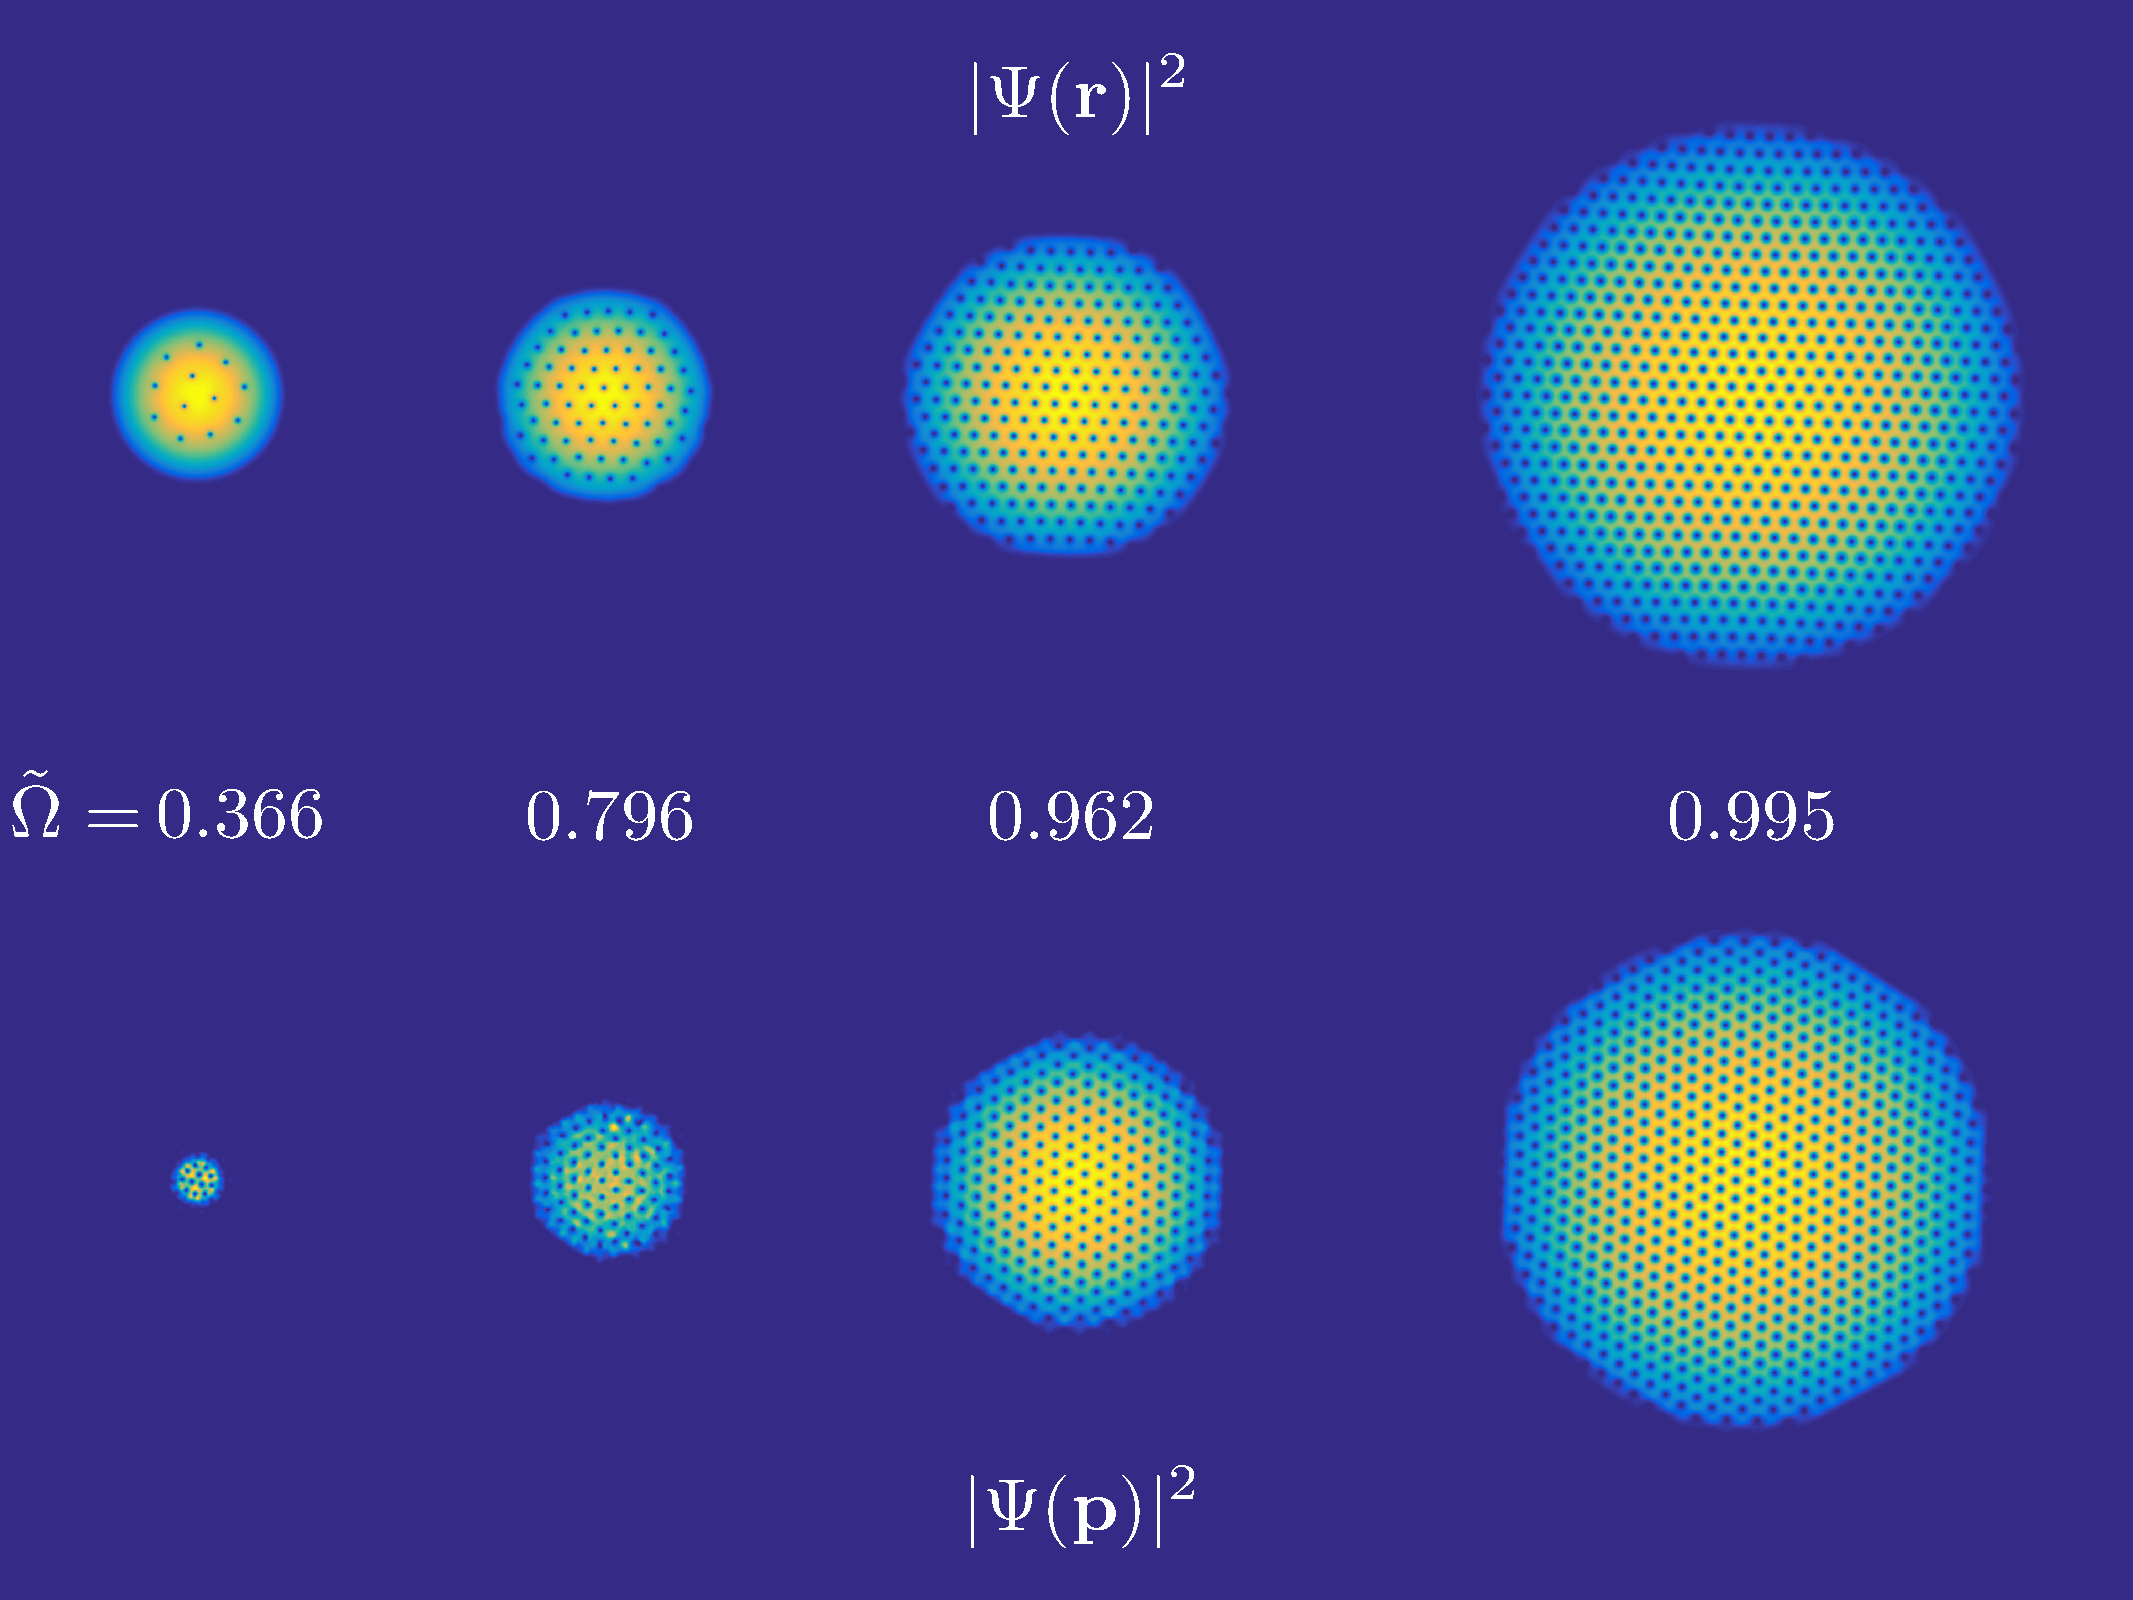
\includegraphics[width=0.85\textwidth]{Images/ch4_vtx/ramp_omega_2.pdf}
    \caption{Density distributions of the wavefunction in position (top) and momentum (bottom) space for increasing rotation frequencies (from left to right). The color axis differs for each plot for visibility, as with a constant axis it is difficult to view densities across all magnitudes. The growth rate of the condensate radius in both position and momentum space becomes large when $\Omega_z \approx \omega_\perp$.}
    \label{fig:inc_omega}
\end{figure}

\begin{figure}\centering
    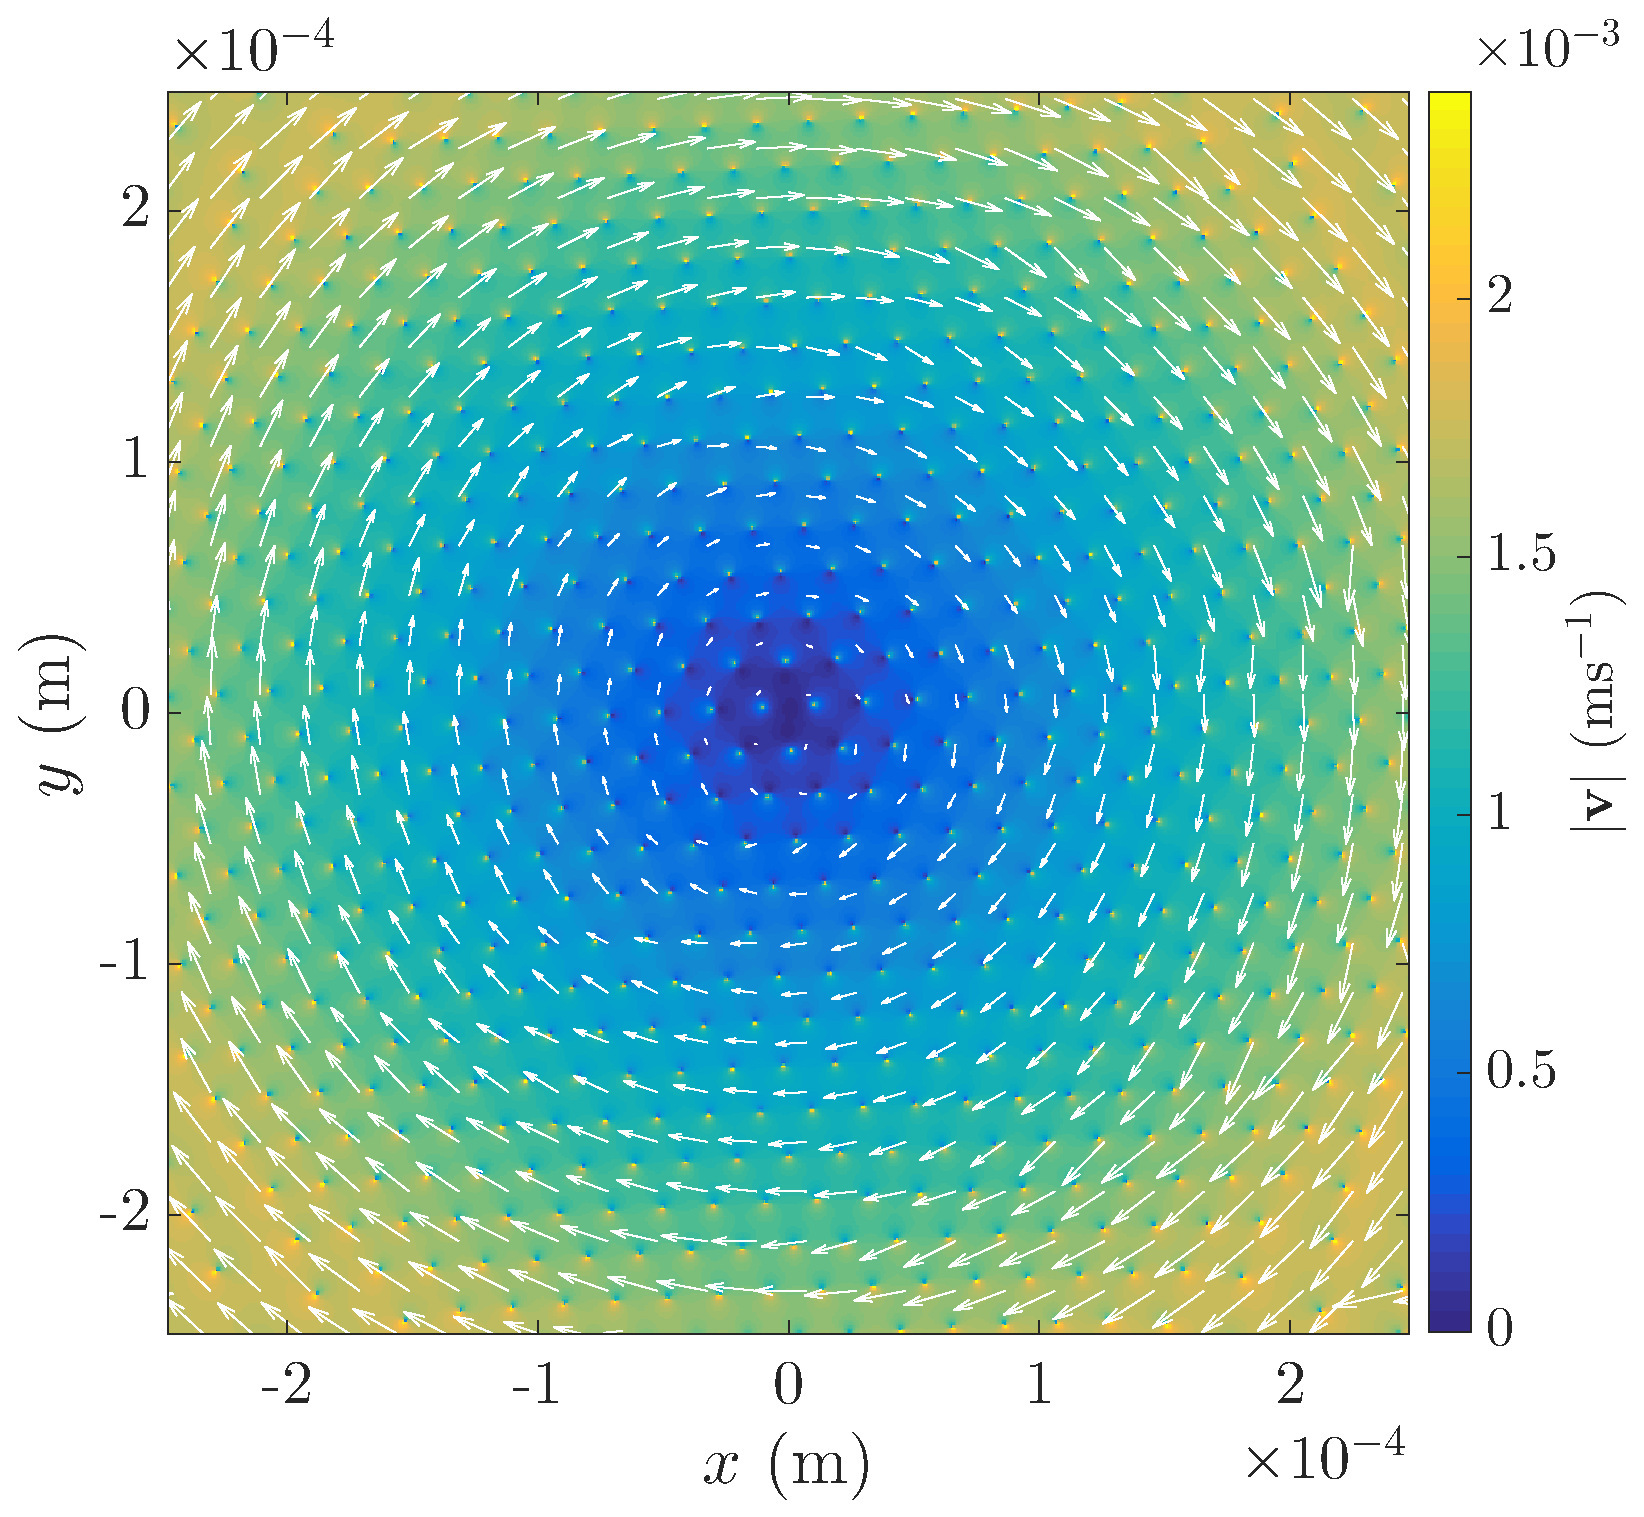
\includegraphics[width=0.47\textwidth,clip,trim={0cm 0cm 0 0cm}]{Images/ch4_vtx/solidbody_v}
    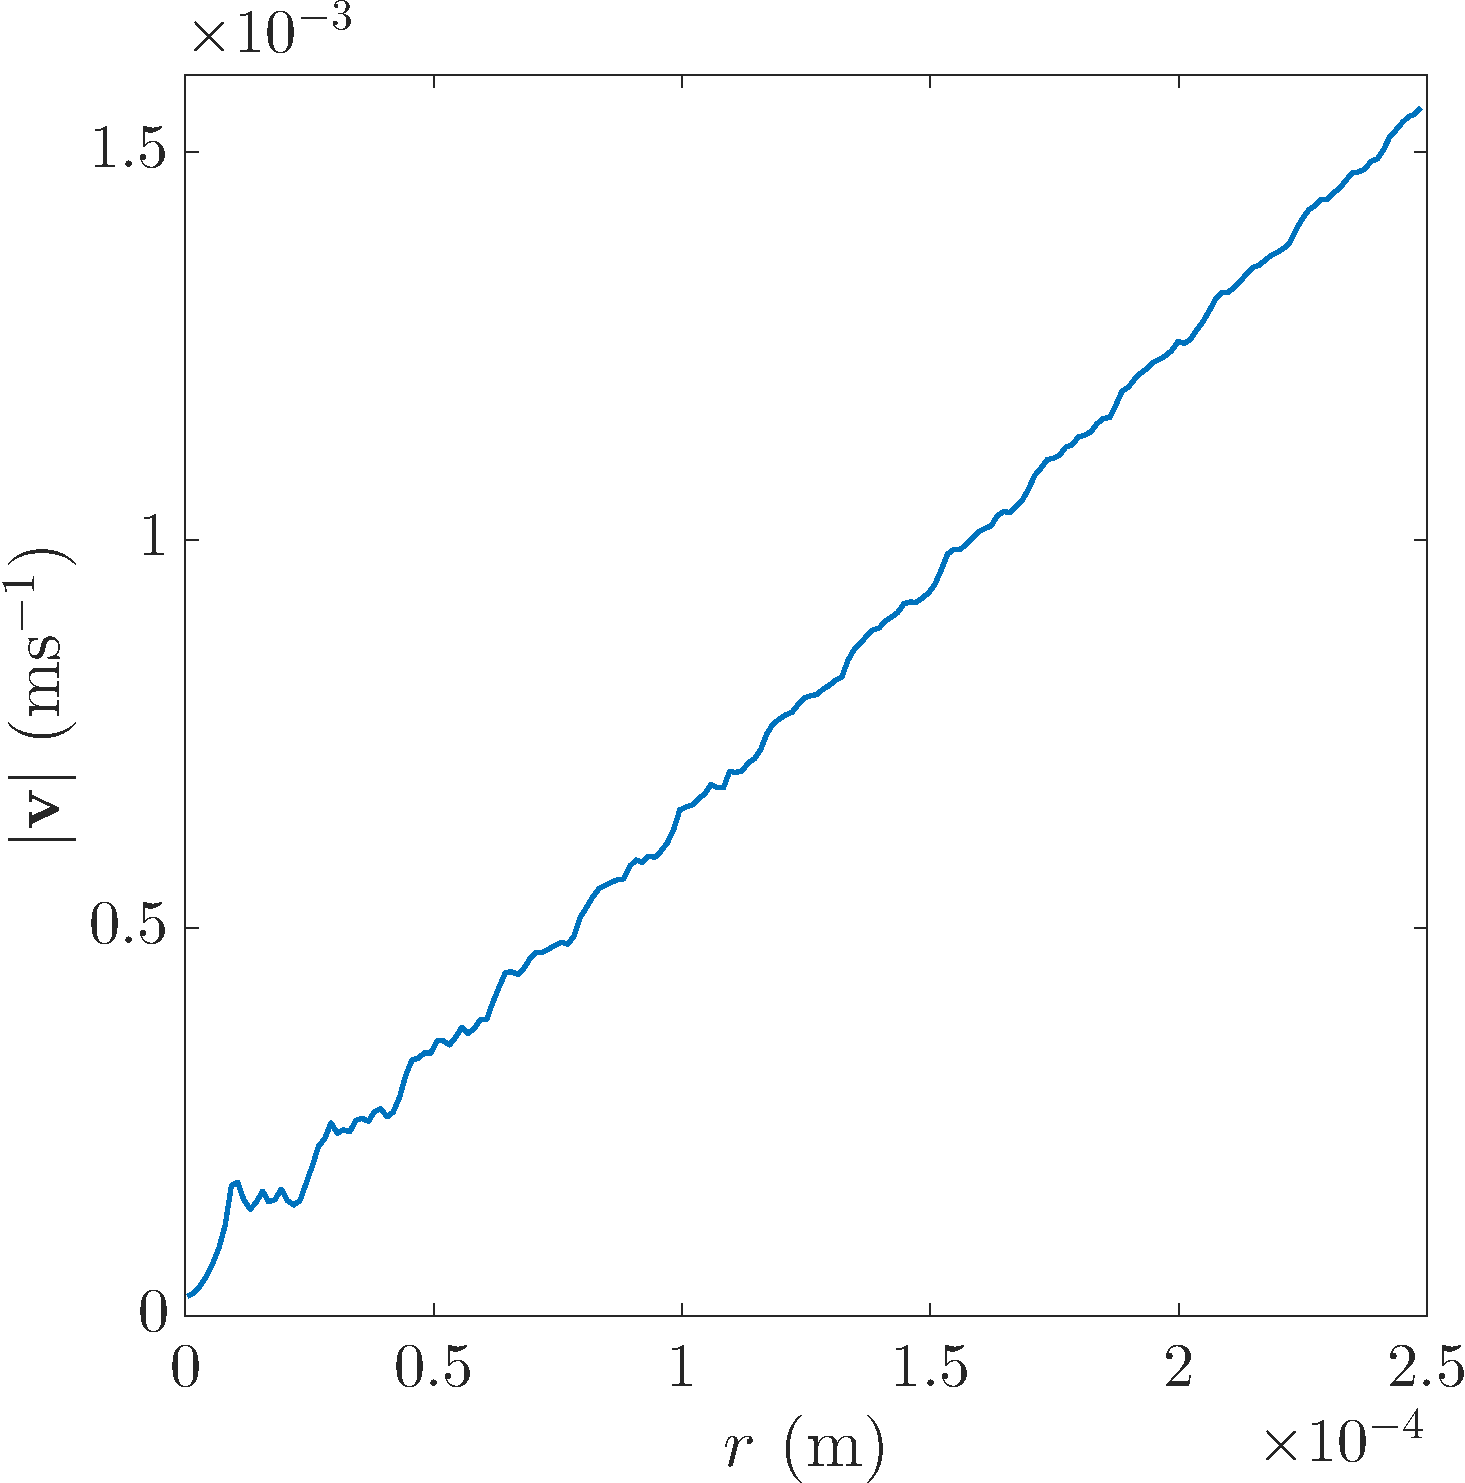
\includegraphics[width=0.43\textwidth,clip,trim={0cm 0cm 0 0cm}]{Images/ch4_vtx/solidbody_vel_r}
    \caption{(Left) Magnitude and direction of flow of the velocity field for a rapidly rotating vortex lattice in the rapidly rotating frame. (Right) The angle-averaged velocity field from condensate centre. The solid-body rotation can be seen, where the coarse-grained condensate velocity scales as $v \propto r$ from the condensate centre. Close to the vortex cores the velocity field retains a $1/r_{\textrm{vtx}}$ profile, becoming singular at the core centres, with $r_{\textrm{vtx}}$ as the distance from the respective cores.}
    \label{fig:solidbody}
\end{figure}

If, however, the linear ramp is performed too quickly, or an initial state is chosen that already contains a large amount of angular momentum without being the eigenstate, the vortices tend to enter from the boundary all at once, and fail to converge to the well ordered groundstate. An example of this such issue is shown in Fig.~\ref{fig:malformed_lattice}, and indicates the need for a slow ramp of $\Omega$ that is essentially adiabatic in imaginary time. As higher rotation frequencies are reached, the rate at which vortices enter the condensate increases rapidly. While the rapid entry of vortices was a problem for reaching an ordered lattice without a ramp of rotation frequency, the presence of an existing lattice during ramping allows all newly entered vortices to order more easily. Therefore, a linear ramp is effective and does not require a more complex scaling.

\begin{figure}
    \centering
    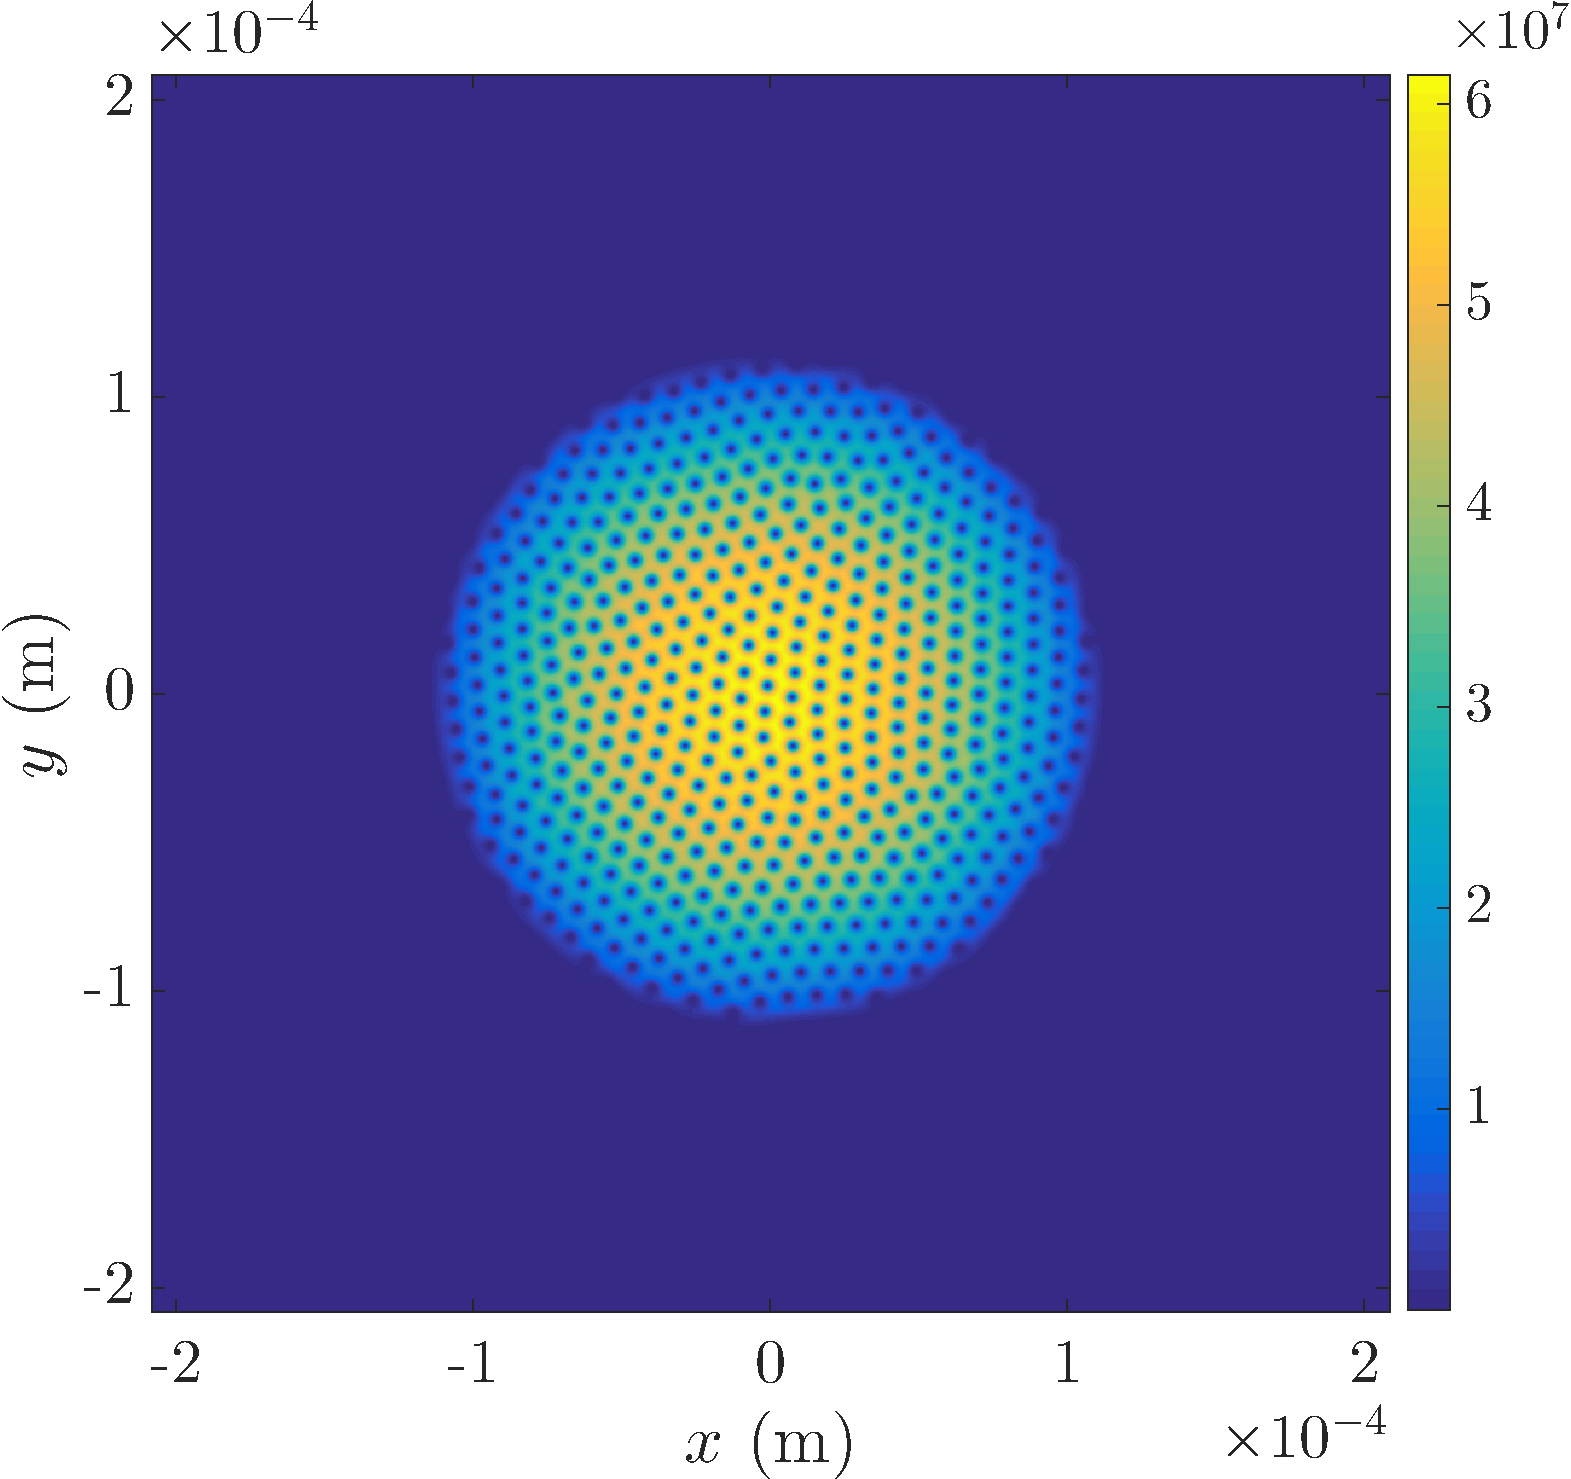
\includegraphics[width=0.65\textwidth]{Images/ch4_vtx/toofast_099_1e7}
    \caption{Disordered lattice resulting from starting in imaginary time evolution at the required rotation rate (here $\Omega=0.99\omega_\perp$). If the rotation frequency is chosen too large without allowing the lattice to form and order, the resulting vortices all enter instantaneously and compete for their final positions. The system only converges one timescales that exceed reasonable computing times.}
    \label{fig:malformed_lattice}
\end{figure}

In the following section we will discuss perturbations of the condensate in the presence and absence of vortices. For the above system, we will investigate the effect of perturbations to both the global and local condensate order due to changes in the lattice structure.

%%%%%%%%%%%%%%%%%%%%%%%%%%%%%%%%%%%%%%%%%%%%%%%%%%%%%%%%%%%% 1
\section{Condensate perturbations}
%%%%%%%%%%%%%%%%%%%%%%%%%%%%%%%%%%%%%%%%%%%%%%%%%%%%%%%%%%%%
%%%%%%%%%%%%%%%%%%%%%%%%%%%%%%%%%%%%%%%%%%%%%%%%%%%%%%%%%%%% a
\subsection{Trapping potential control}\label{ss:pert_opt_latt}
%%%%%%%%%%%%%%%%%%%%%%%%%%%%%%%%%%%%%%%%%%%%%%%%%%%%%%%%%%%%
With the model system outlined in Sec.~\ref{sec:modelsystem}, we will now imagine an abrupt change to the Hamiltonian, such that, $H(t) = H_{\textrm{GP}} + f(t) V_{\textrm{ext}}$, where $V_{\textrm{ext}}$ is an external potential, and $f(t)$ is some function of time to control the application of $V_{\textrm{ext}}$. In this scenario the initial wavefunction, which is a stationary state of $H_{\textrm{GP}}$, will no longer remain so provided that $H_{\textrm{GP}}$ and $f(t) V_{\textrm{ext}}$ are non-commuting. Assuming the time of application of the additional term is much shorter than any other timescale of the condensate dynamics, any modification of the Hamiltonian in this way can be viewed as a method for changing the phase of the wavefunction.
%\begin{equation}
%    e^{i\phi} \mapsto \exp\left(-i\frac{Ht}{\hbar}\right),
%\end{equation}
The resulting effect on the wavefunction can be given as
\begin{subequations}
\begin{align}
    \Psi(t=0) &= |\Psi(t=0)|e^{\textrm{i}\theta_0} \\
    \Psi(t) &= \Psi(t=0) e^{ - \textrm{i} \frac{ V_{\textrm{ext}} \Delta t}{\hbar}} \\
            &= |\Psi(t=0)| e^{\textrm{i}\left(\theta_0 - \frac{V_{\textrm{ext}} \Delta t}{\hbar}\right)} \nonumber
\end{align}
\end{subequations}
where we have made use of Eq.~\eqref{eqn:madelung}. After application of $V_{\textrm{ext}}$ the wavefunction phase is given by
\begin{equation}
    \theta^{'} = \theta_0 - \frac{E_{\textrm{ext}} \Delta t}{\hbar},
\end{equation}
where $E_{\textrm{ext}}$ is the perturbance energy. One commonly used method to manipulate the condensate is through the use of optical potentials, which offer a large degree of control over the respective system's Hamiltonian \cite{BEC:Bloch_revmodphys_2008}. The electric field component of an arbitrary optical field, described by a wavevector $\mathbf{k}$, and frequency, $\omega$ is given by
\begin{equation}
    \mathbf{E}(\mathbf{r},t) = \varepsilon_0 e^{\textrm{i}\left(\mathbf{k}\cdot\mathbf{r} - \omega t\right)} + \ \varepsilon_0^{*} e^{-\textrm{i}\left(\mathbf{k}\cdot\mathbf{r} - \omega t\right)},
\end{equation}
where $\varepsilon_0$ is the field amplitude. Using the dipole approximation, the interaction of an atom with a laser field is given by~\cite{BK:Foot_2005}
\begin{equation}
\mathcal{V} = -{\mathbf{d}}\cdot {\mathbf{E}},
\end{equation}
where ${\mathbf{d}}$ is the electric dipole moment operator. For a two level atom with a groundstate $| g \rangle$, and an excited state $| e \rangle$ with energy difference $\hbar \omega_0$, the dipole operator can be written as
\begin{align}\label{eqn:dipole_approx}
\mathbf{d} &= \langle g|\mathbf{d}|e \rangle | g \rangle \langle e | + \langle e|\mathbf{d}|g \rangle | e \rangle \langle g | \nonumber \\
&= \boldsymbol{\mu}_{eg} | g \rangle \langle e | + \boldsymbol{\mu}_{eg}^{*} | e \rangle \langle g |,
\end{align}
where we have made use of $\langle g|\mathbf{d}|g \rangle = \langle e|\mathbf{d}|e \rangle  = 0$, since the atoms have no permanent dipole moment. From Eq.~\eqref{eqn:dipole_approx} the Hamiltonian of the two-level system can then be written as
\begin{align}\label{eqn:dip_hamiltonian}
    H &= H_0  - \mathcal{V} \nonumber \\
      &=  \hbar\omega_0 |e\rangle\langle e | - (\boldsymbol{\mu}_{eg} | g \rangle \langle e | + \boldsymbol{\mu}_{eg}^{*} | e \rangle \langle g |)\cdot ( \varepsilon_0 e^{\textrm{i}\left(\mathbf{k}\cdot\mathbf{r} - \omega t\right)} +  \varepsilon_0^{*} e^{-\textrm{i}\left(\mathbf{k}\cdot\mathbf{r} - \omega t\right)}).
\end{align}
After expanding~\eqref{eqn:dip_hamiltonian} we can then rewrite $\boldsymbol{\mu}_{eg}\cdot \varepsilon_0 = \hbar\Omega_r$, where $\Omega_r$ is the Rabi-oscillation frequency between the states. Assuming that the detuning $\Delta = \omega - \omega_0$ between the laser field and transition frequency is small, $\Delta \ll \omega + \omega_0$, allows use of the rotating wave approximation. For this we first perform a unitary transformation of the system into the interaction picture rotating with $H_0$ using the operator $U = e^{-\textrm{i}\omega_0 t|e\rangle\langle e|}$ as
\begin{align}
    H_{\textrm{int}} & = U^{\dagger} \mathcal{V} U.
\end{align}
All resulting terms featuring $\omega + \omega_0$ can be considered to be rapidly oscillating, and average out to zero. Following this approximation, the Hamiltonian can be transformed back into the Schr\"odinger picture, giving
\begin{align}
 H^{'} = \hbar\omega_0 - \hbar\Omega\left(e^{-\textrm{i}\omega t}|e\rangle\langle g|   + e^{\textrm{i}\omega t}|g\rangle\langle e|  \right).
\end{align}
The final shift of the energies is then given as
\begin{equation}\label{eqn:acshift}
\mathcal{V} = -\frac{\alpha}{2}\langle \mathbf{E}^2\rangle_t ,
\end{equation}
where $\alpha$ is the real component of the atomic polarisability, and $\langle \cdot \rangle_t$ denotes the time average. If the electric field is spatially inhomogeneous, then this leads to a force of the form
\begin{equation}
\mathbf{F}_d = -\frac{\alpha}{2}\nabla\langle \mathbf{E}^2 \rangle_t ,
\end{equation}
which is known as the dipole force. Assuming counter propagating plane waves, we can then model a standing wave solution of the resulting optical potential as
\begin{equation}
    V_{\textrm{ext}} \approx -\frac{\Omega_0^2(\mathbf{r})}{4\Delta}  = V_0 \cos^2 (\mathbf{k} \cdot \mathbf{r}),
\end{equation}
where $V_0 = -\Omega_0^2/4\Delta$ is the field intensity, and $\Omega_0 \propto |\varepsilon_0|^2$ is the Rabi-frequency of the standing wave. The optical potential forms a highly periodic system given an appropriately chosen $\mathbf{k}$, and is known as an \textit{optical lattice}. Optical lattices have become very common in BEC experiments as they allow for control of the kinetic energy term of the atoms to a very high degree~\cite{OL:Greiner_nat_2002,OL:Reijnders_prl_2004,OL:Sorensen_prl_2005,Vtx:Tung_prl_2006,Vtx:Vignolo_pra_2007,BEC:Watanabe_entropy_2016}.

%The optical lattice potential can be used to create one, two, or three-dimensional periodic trapping structures.
%\todo[inline]{Add full optical potential including polarisation terms}
Different geometric potentials can be formed with optical lattices by using laser fields with different $\mathbf{k}$ vectors. Assuming standing waves with different polarisation axes or slightly different wavelengths, the interference effects between two or more fields can be ignored, with the resulting optical field given by the summation of lattice potentials with wavevectors $\mathbf{k}_{1,..,n}$. Creating a 2D lattice with $n$-fold rotational symmetry requires $n/2$ $\mathbf{k}$-vectors separated by $\frac{2\pi}{n}$, and with $n/2 \in \mathbb{Z}^{+}$. Taking a square lattice as an example, which has a 4-fold rotational symmetry, it can be created by two $\mathbf{k}$-vectors, separated by $\pi/2$, as
\begin{equation}
    \mathbf{k}_0 = \left[ \begin{array}{cc}
    1 \\
    0
    \end{array} \right],~
    \mathbf{k}_1 =
    \left[ \begin{array}{cc}
     0 \\
     1
    \end{array} \right].\label{eqn:sqlatt}
\end{equation}
The resulting potential is shown in Fig.~\ref{fig:cos2xy}.
\begin{figure}\centering
    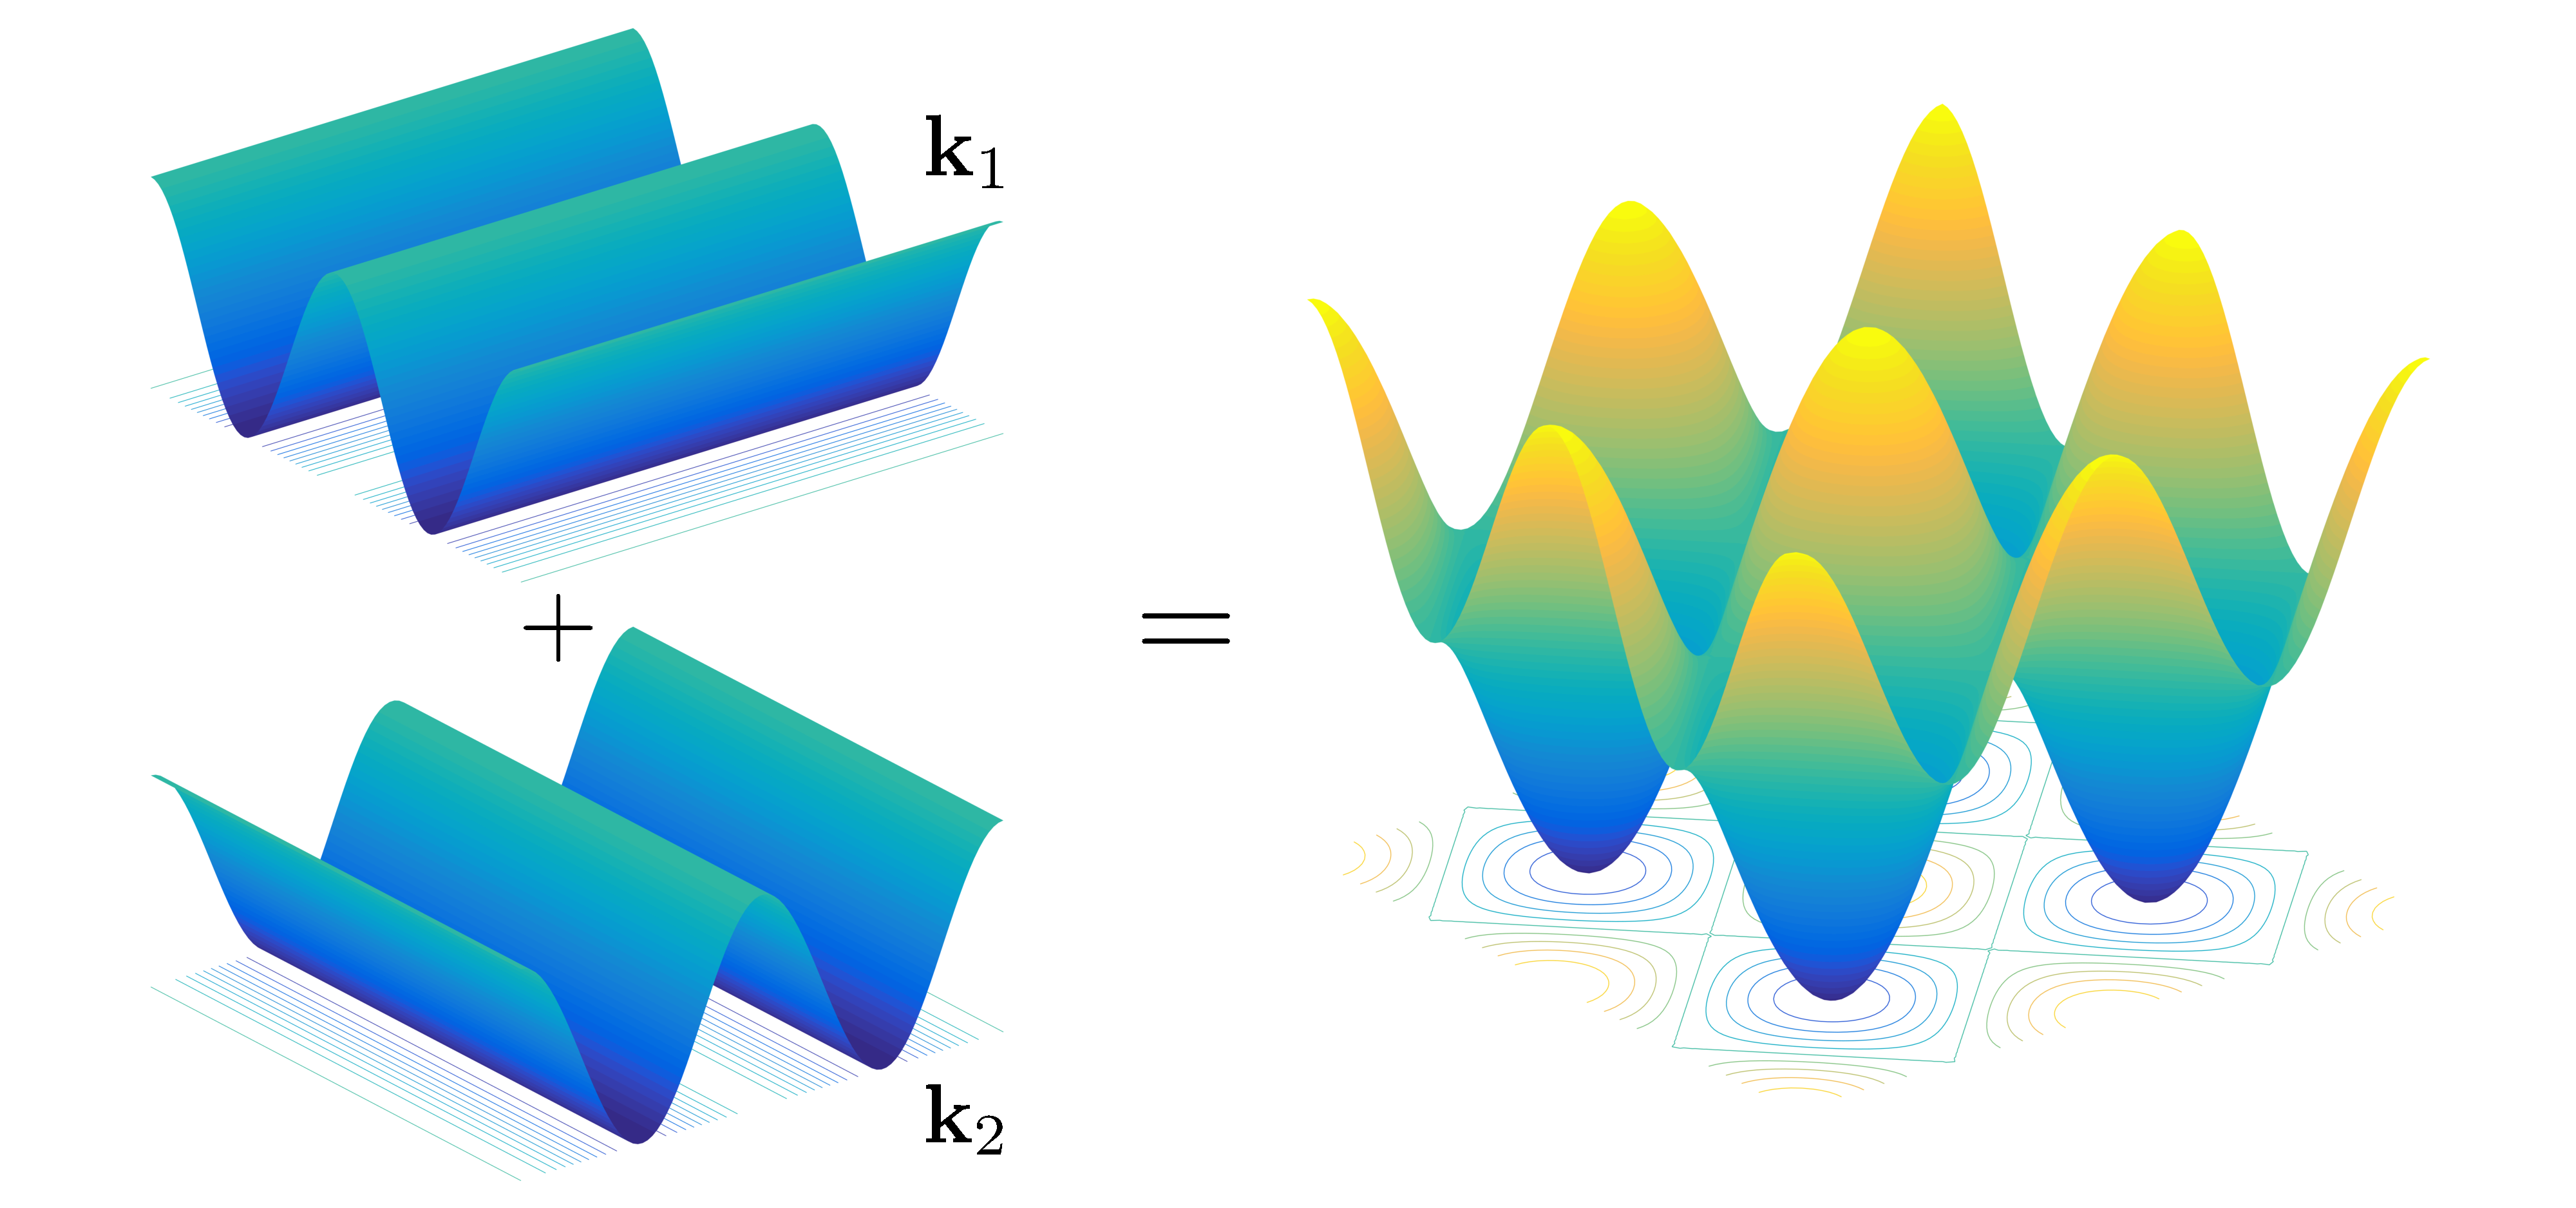
\includegraphics[width=0.55\textwidth]{./Images/ch4_vtx/VOPT/squarelatt}
    \caption{Square lattice generation using two orthogonal propagating laser fields with wavevectors $\mathbf{k}_1$ and $\mathbf{k}_2$, as defined by Eq.~\eqref{eqn:sqlatt}.}\label{fig:cos2xy}
\end{figure}
The time the optical lattice is applied to the condensate can be controlled by choosing the function $f(t)$. Applying a lattice for a finite, but short, time only will lead to a modification of the wavefunction phase, which then subsequently, and on a much longer time-scale, will have an effect on the density distribution. Of particular interest to us is the use of an optical potential that is pulsed one or several times, which can be described by $f(t)$ as a periodic delta function. The condensate phase profile is the only quantity immediately modified, and any change in the density distribution appears only in the following evolution.

\iffalse
For the purpose of my system, we intend to create a two-dimensional optical lattice, wherein the structure of the lattice matches that of the triangular Abrikosov vortex pattern. The triangular lattice has 6-fold rotational symmetry, and can be formed with wavevectors

\begin{subequations}
    \begin{align}
        \mathbf{k}_1 &= k_0\left\{\frac{\sqrt(3)}{2},\frac{1}{2}\right\} \\
        \mathbf{k}_2 &= k_0\{0,1\} \\
        \mathbf{k}_3 &= k_0\left\{\frac{\sqrt(3)}{2},-\frac{1}{2}\right\} \\
    \end{align}
\end{subequations}
where $k_0 = 4\pi/(\sqrt(3)a_\text{O})$, and $a_\text{O}$ is the lattice spacing.
\fi


%%%%%%%%%%%%%%%%%%%%%%%%%%%%%%%%%%%%%%%%%%%%%%%%%%%%%%%%%%%% b
\subsection{Direct phase manipulation}\label{sec:phase}
%%%%%%%%%%%%%%%%%%%%%%%%%%%%%%%%%%%%%%%%%%%%%%%%%%%%%%%%%%%%

While groundstate condensates will have a flat phase across the system, there are two interesting examples where a spatially dependent phase exists: dark solitons~\cite{BEC:Denschlag_science_2000} and vortices~\cite{Vtx:Dobrek_pra_1999}. We have previously discussed the $2\pi$ phase profile of a vortex that leads to the singularities in the wavefunction. In contrast, dark solitons feature a $\pi$ phase jump profile. These excitations are unstable in dimensions higher than one, and will decay via the snake instability to paired vortices and antivortices~\cite{BEC:Brand_pra_2002}. Where so far we have only considered the short-term evolution of the wavefunction after being kicked by an optical potential, we will in the following consider what structures can be created in the condensate by careful phase manipulation techniques, besides dark solitons and vortices.

For this we will assume that the BEC allows for a short enough application of potentials so that only the phase is affected, and discuss direct manipulation of the wavefunction, as opposed to modification of the Hamiltonian. Following \cite{BK:Pitaevskii_Stringari_2003} and taking Eq.~\eqref{eqn:madelung}, the phase of the condensate can then be written as
\begin{equation}
\theta = \theta_0 + \theta_i,
\end{equation}

where $\theta_0$ is the unperturbed condensate phase, and $\theta_i$ is the phase pattern to be imprinted. Upon solving for the initial condensate groundstate with deterministic phase, an additional phase pattern can be imprinted at any time by simply multiplying the wavefunction by $e^{\text{i}\theta_i}$. However, without careful choice of the phase terms their addition can lead to unwanted dynamics, so care must be taken to choose a well defined initial and imprinted phase pattern.

The advantage of the phase imprinting model is that for topological defects, one can imprint the required winding instantaneously, allowing them to appear at predefined positions. The density also needs to only adjust itself locally to the phase singularity, with the remaining condensate seeing an almost constant shift in phase. The creation of vortices through application of localised $\pm 2\pi$ phase winding defects in the condensate therefore allows for direct control of the angular momentum and vorticity within the BEC. While discussed in the literature for the creation of vortices, it is worth noting that the phase imprinting method can also be used to annihilate a vortex from the condensate by applying a phase profile of opposite winding, removing the singularity. This will leave the condensate with a density depletion at the prior location of the phase singularity. Without the phase singularity this depletion will fill in and excite phonon modes in the condensate during time evolution. This process will form the basis for further discussions and analysis of vortex carrying condensates.

Experimental realisation of arbitrary potential patterns to achieve the required phase is accessible through the use of spatial light modulators (SLM)~\cite{VTX:Moulder_pra_2012}. These devices behave as digital displays, through which visual patterns can be expressed in a time dependent manner, allowing the application of a laser field in the required form. We will assume for all future discussions that the potentials we require are experimentally realisable with sufficient resolution, and focus on the resulting effect on the condensate. For the creation of a single vortex the $2\pi$ phase winding pattern can be created spatially using the two-argument four-quadrant form of $\arctan$ as given by
\begin{equation}
    \theta_i(\mathbf{x},\mathbf{y};x_0,y_0) = \arctan(\mathbf{y}-y_0,\mathbf{x}-x_0),
\end{equation}
which locates the singularity at the position $\left(x_0,y_0\right)$. The resulting phase is shown in Fig.~\ref{fig:atan2phase}(left), and including the additional phase singularity term $\theta_i$, the condensate wavefunction following an imprint is given as
\begin{equation}
    \Psi^{'}(\mathbf{r},t) = |\Psi(\mathbf{r},t)|e^{\text{i}(\theta_0(\mathbf{r},t) + \theta_i(\mathbf{r}))}.
\end{equation}

\begin{figure}\centering
    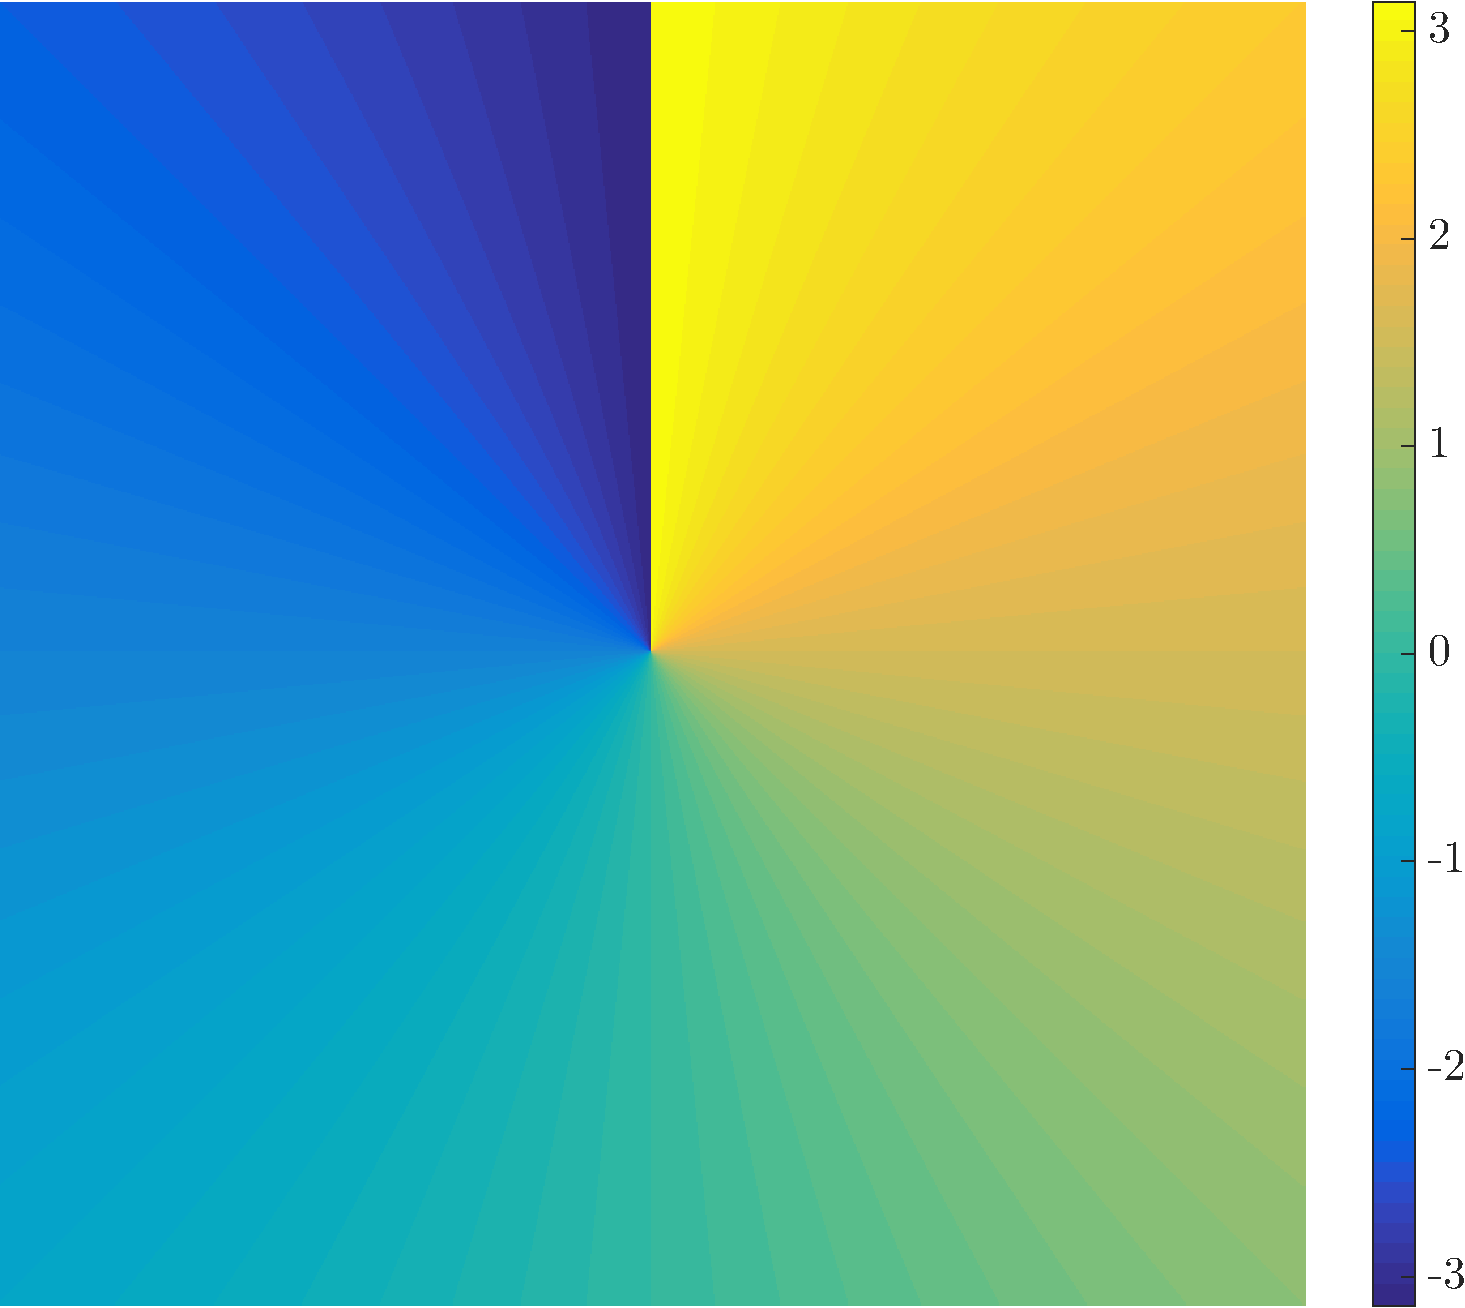
\includegraphics[width=0.45\textwidth]{Images/ch4_vtx/2pi.pdf}
    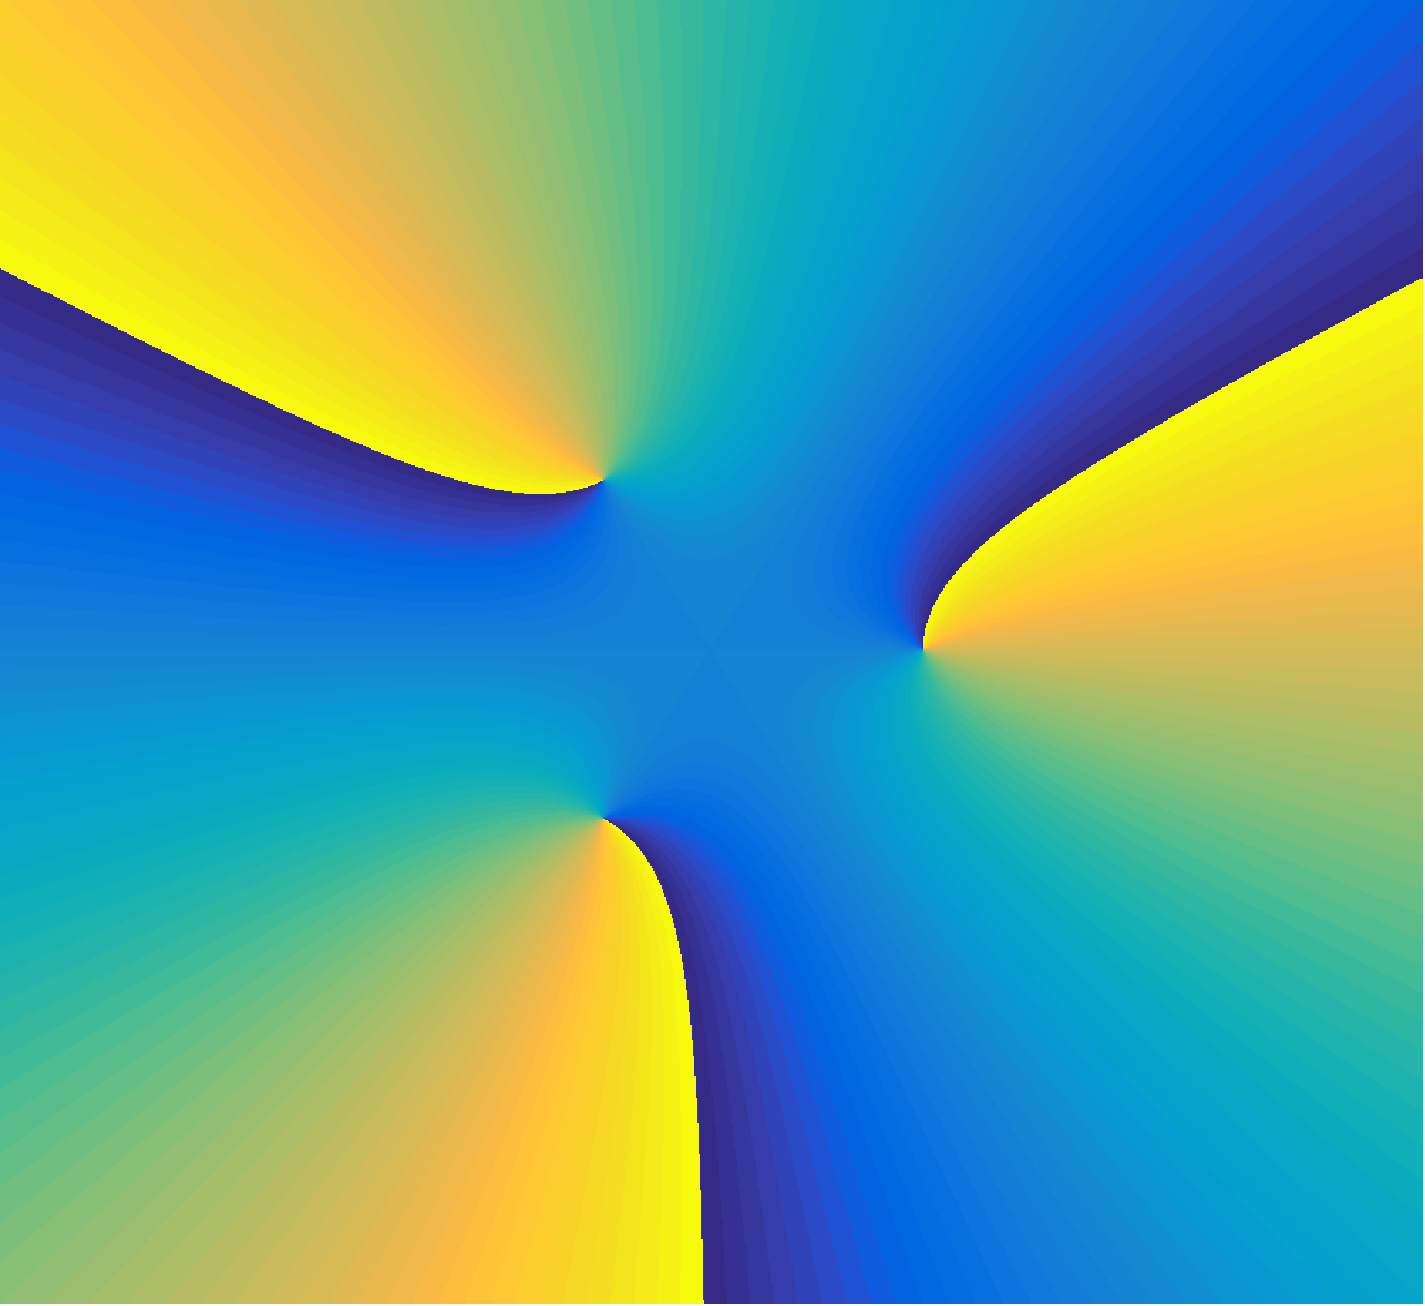
\includegraphics[width=0.435\textwidth]{Images/ch4_vtx/3_2pi.pdf}
    \caption{$2\pi$ phase winding shown for a single (left) and three separated (right) phase singularities. The application of separate phase singularities can be treated as summing each individual phase profile, $\left(\displaystyle\sum\limits_i \theta_i \right)\mod 2\pi$. Note that the resolution used in the numerical examples is much higher than can be obtained from currently available SLMs.}\label{fig:atan2phase}
\end{figure}

Following the imprint this process will create phonons in the condensate density that will radiate outwards from the singularity imprint. As imprinting is directly controlling the condensate phase, it can also be considered a direct manipulation of the kinetic energy since the superfluid velocity depends on the phase gradient (see Eq.~\eqref{eqn:velocity}). This, in reverse, means that by applying spatially inhomogeneous phase profiles the atomic velocity can be adjusted to different values in different regions of the condensate. To demonstrate this we consider a simple example of a Gaussian phase profile applied to the condensate. The imprinted profile has the form
\begin{equation}
    \theta_{i}(\mathbf{r}) = A\exp\left( -\frac{ |\mathbf{r}-\mathbf{r}_0|^2 }{2\sigma^2 } \right) \mod 2\pi,
\end{equation}
where $A$ is the phase profile amplitude, $\mathbf{r}_0$ is the centre of the Gaussian curve, and $\sigma$ is adjusted to match the condensate width. The modulo $2\pi$ ensures that the phase wraps around for amplitudes exceeding the $(0,2\pi)$ range. The Gaussian profile has large radial gradients in two-dimensions, so that an imprint on the condensate should lead to radial velocities and therefore an expansion or contraction of the cloud (see Fig.~\ref{fig:gaussian}). This can be expected to lead to interference fringes, as the faster moving atoms have the possibility to overtake the slower ones for sufficiently large amplitudes~\cite{BEC:Busch_pra_2002}. In Fig.~\ref{fig:gaussian_wfc}, where a slice through the condensate centre is given for both position and momentum space, this can be clearly seen.

\begin{figure}\centering
    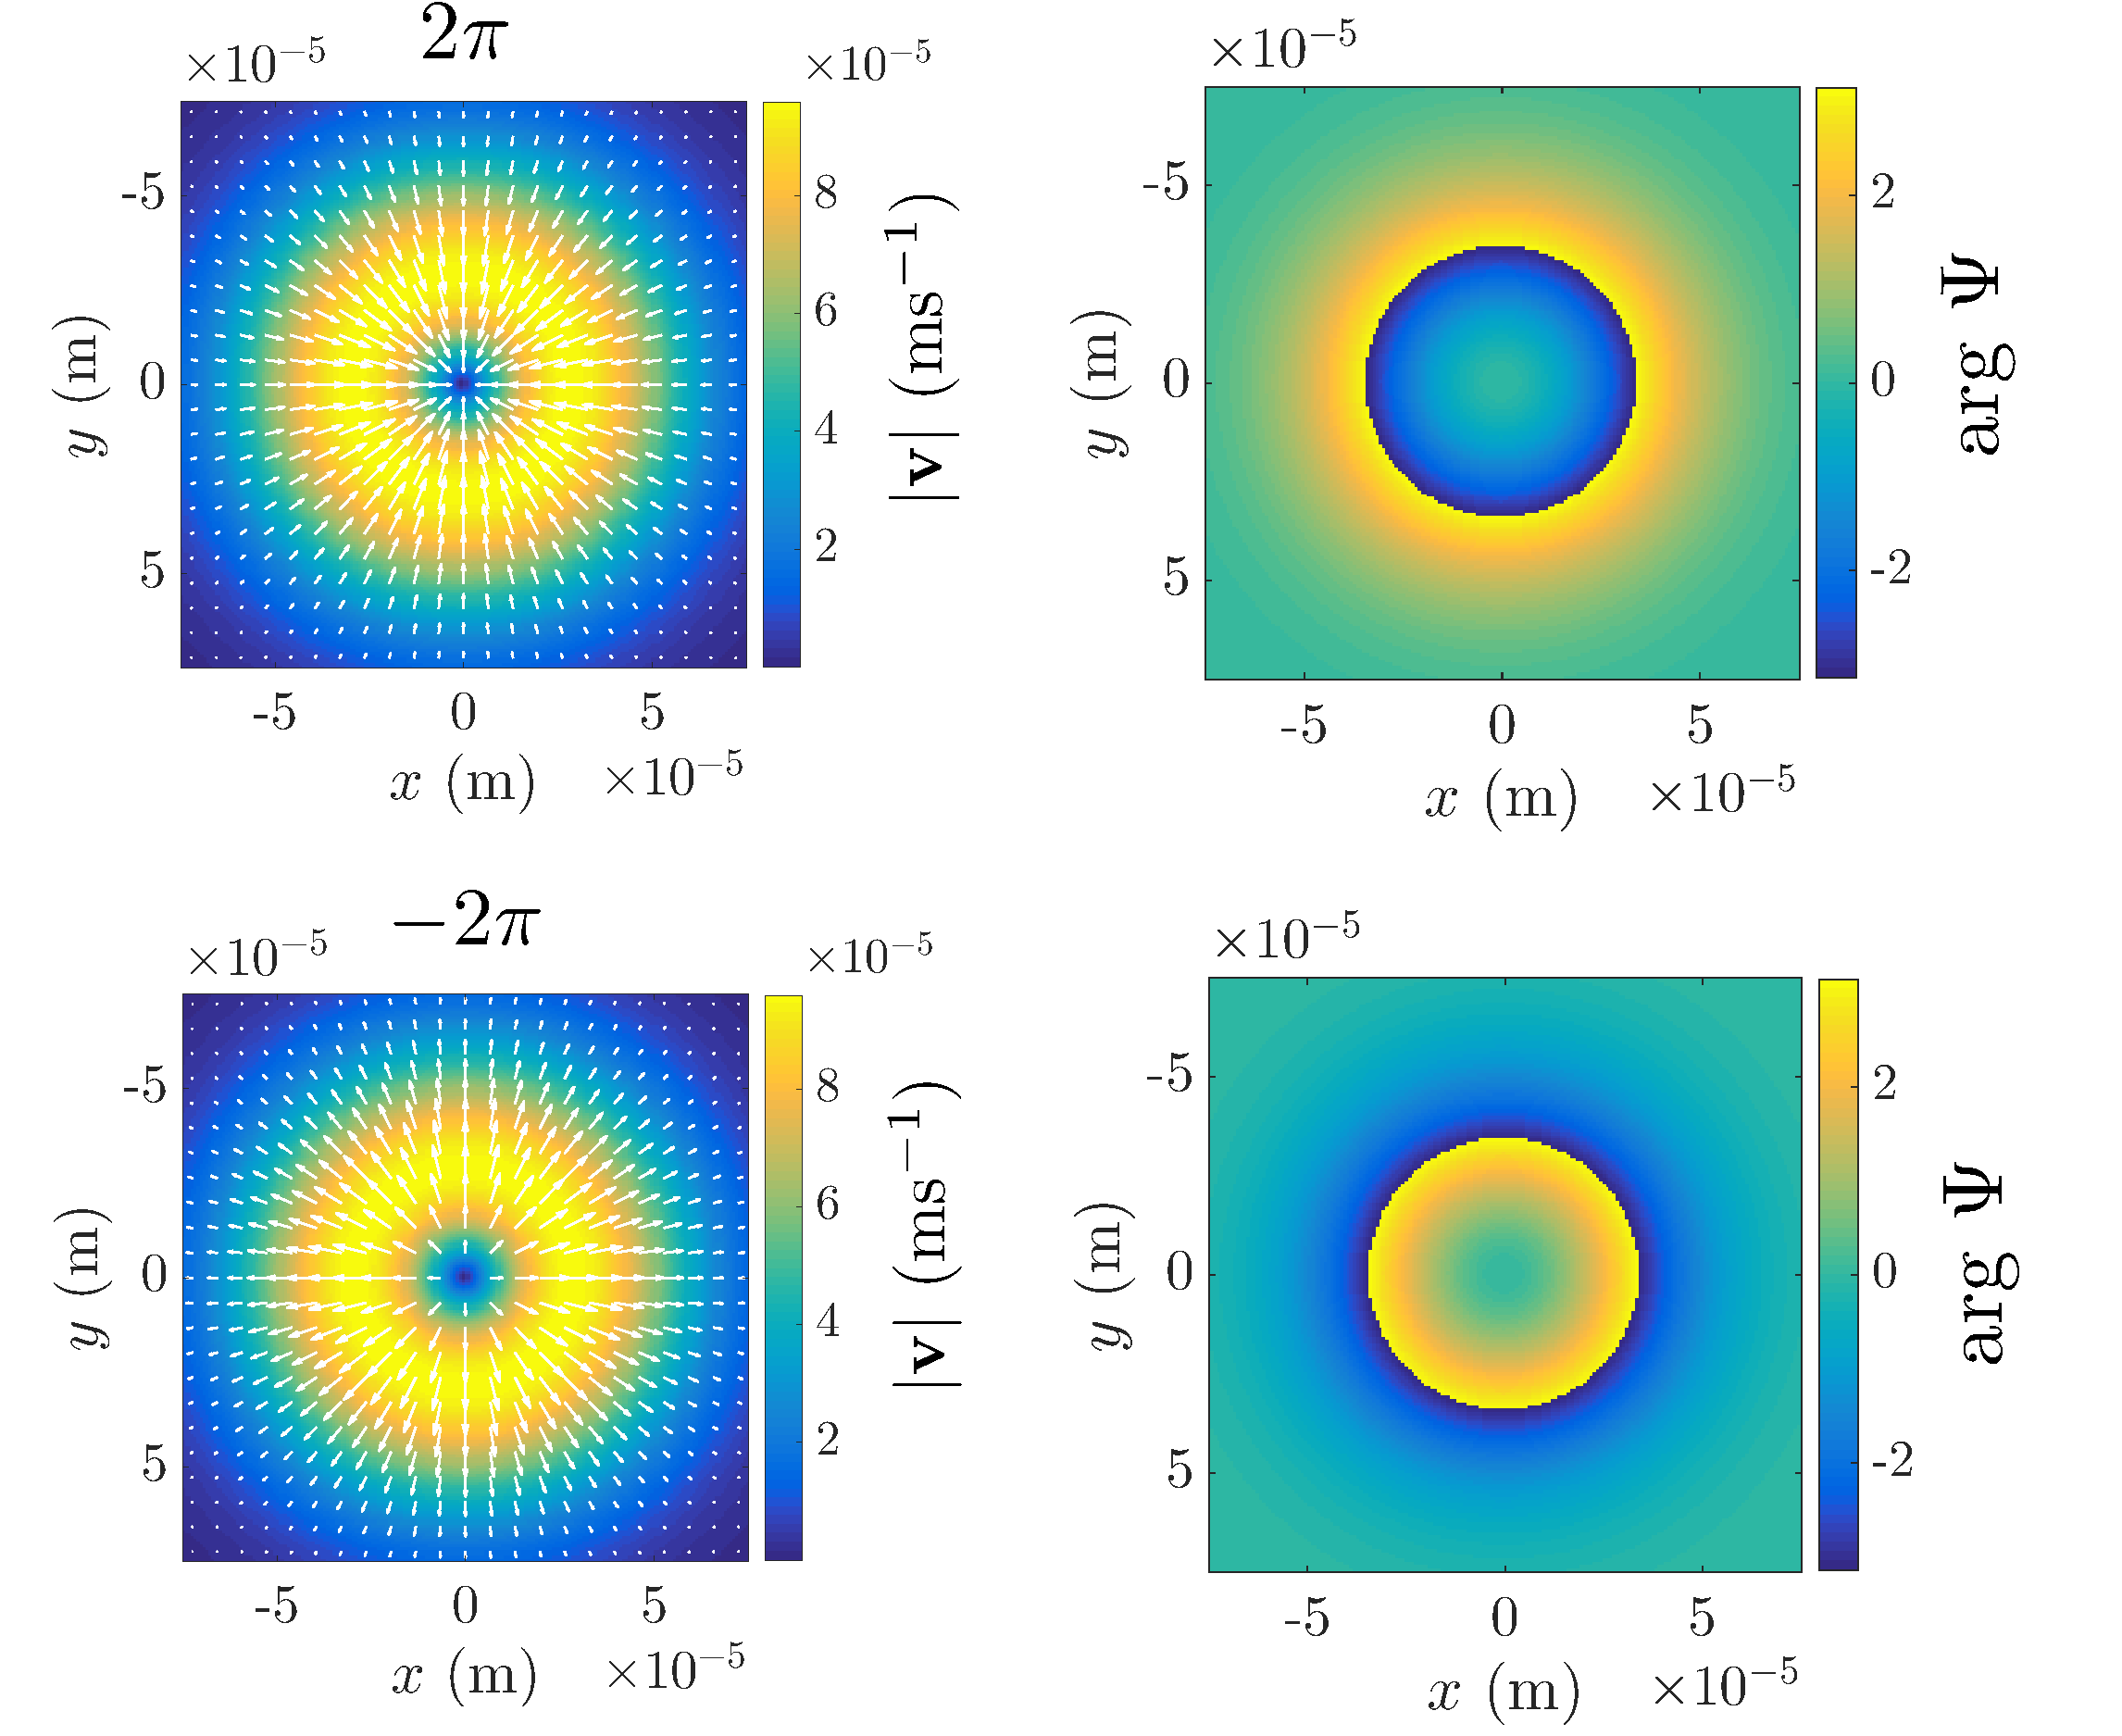
\includegraphics[width=0.95\textwidth]{Images/ch4_vtx/velocity/gaussian_imprint}
    \caption{Velocity fields and magnitude (left) and phase (right) for a condensate directly following a Gaussian phase imprint. The lengths of the arrows give the magnitude of the respective velocity components, with the color map indicating this also for clarity. The sign of the imprint changes the direction of the respective kinetic components, with a positive imprint initially creating a density contraction (top), and negative creating an expansion (bottom), with the arrows indicating the direction of the flow.}\label{fig:gaussian}
\end{figure}

\begin{figure}\centering
    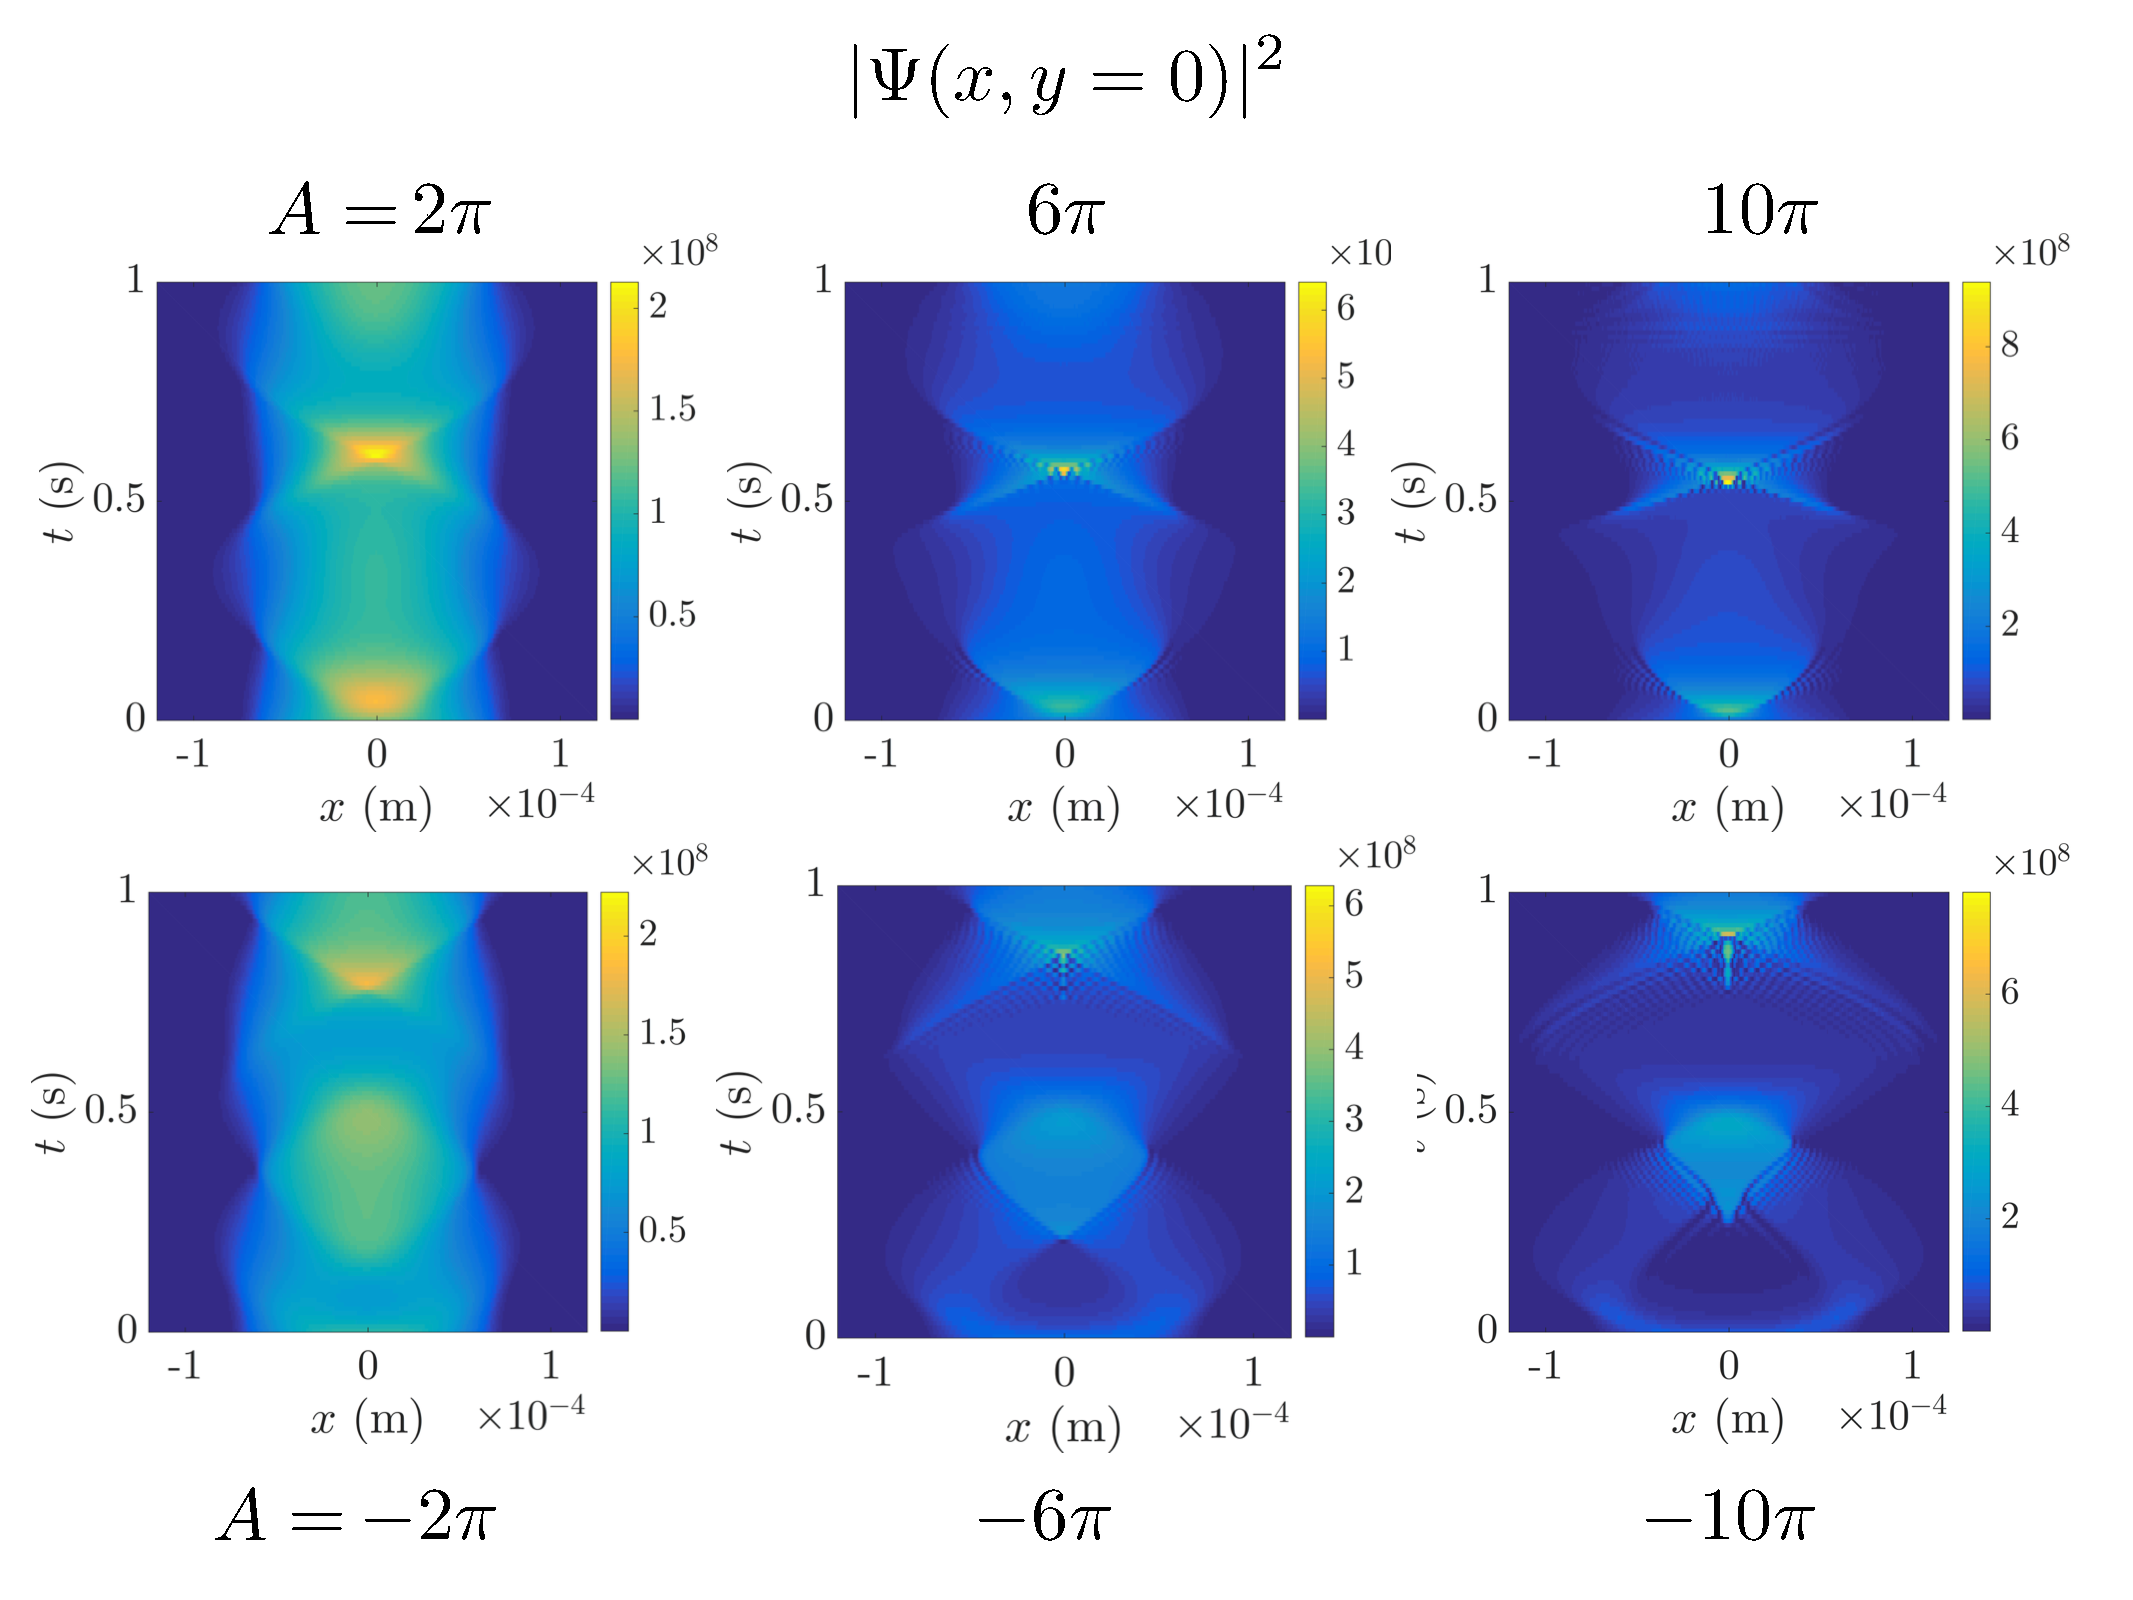
\includegraphics[width=0.95\textwidth]{Images/ch4_vtx/gaussian_imprint_B}
    %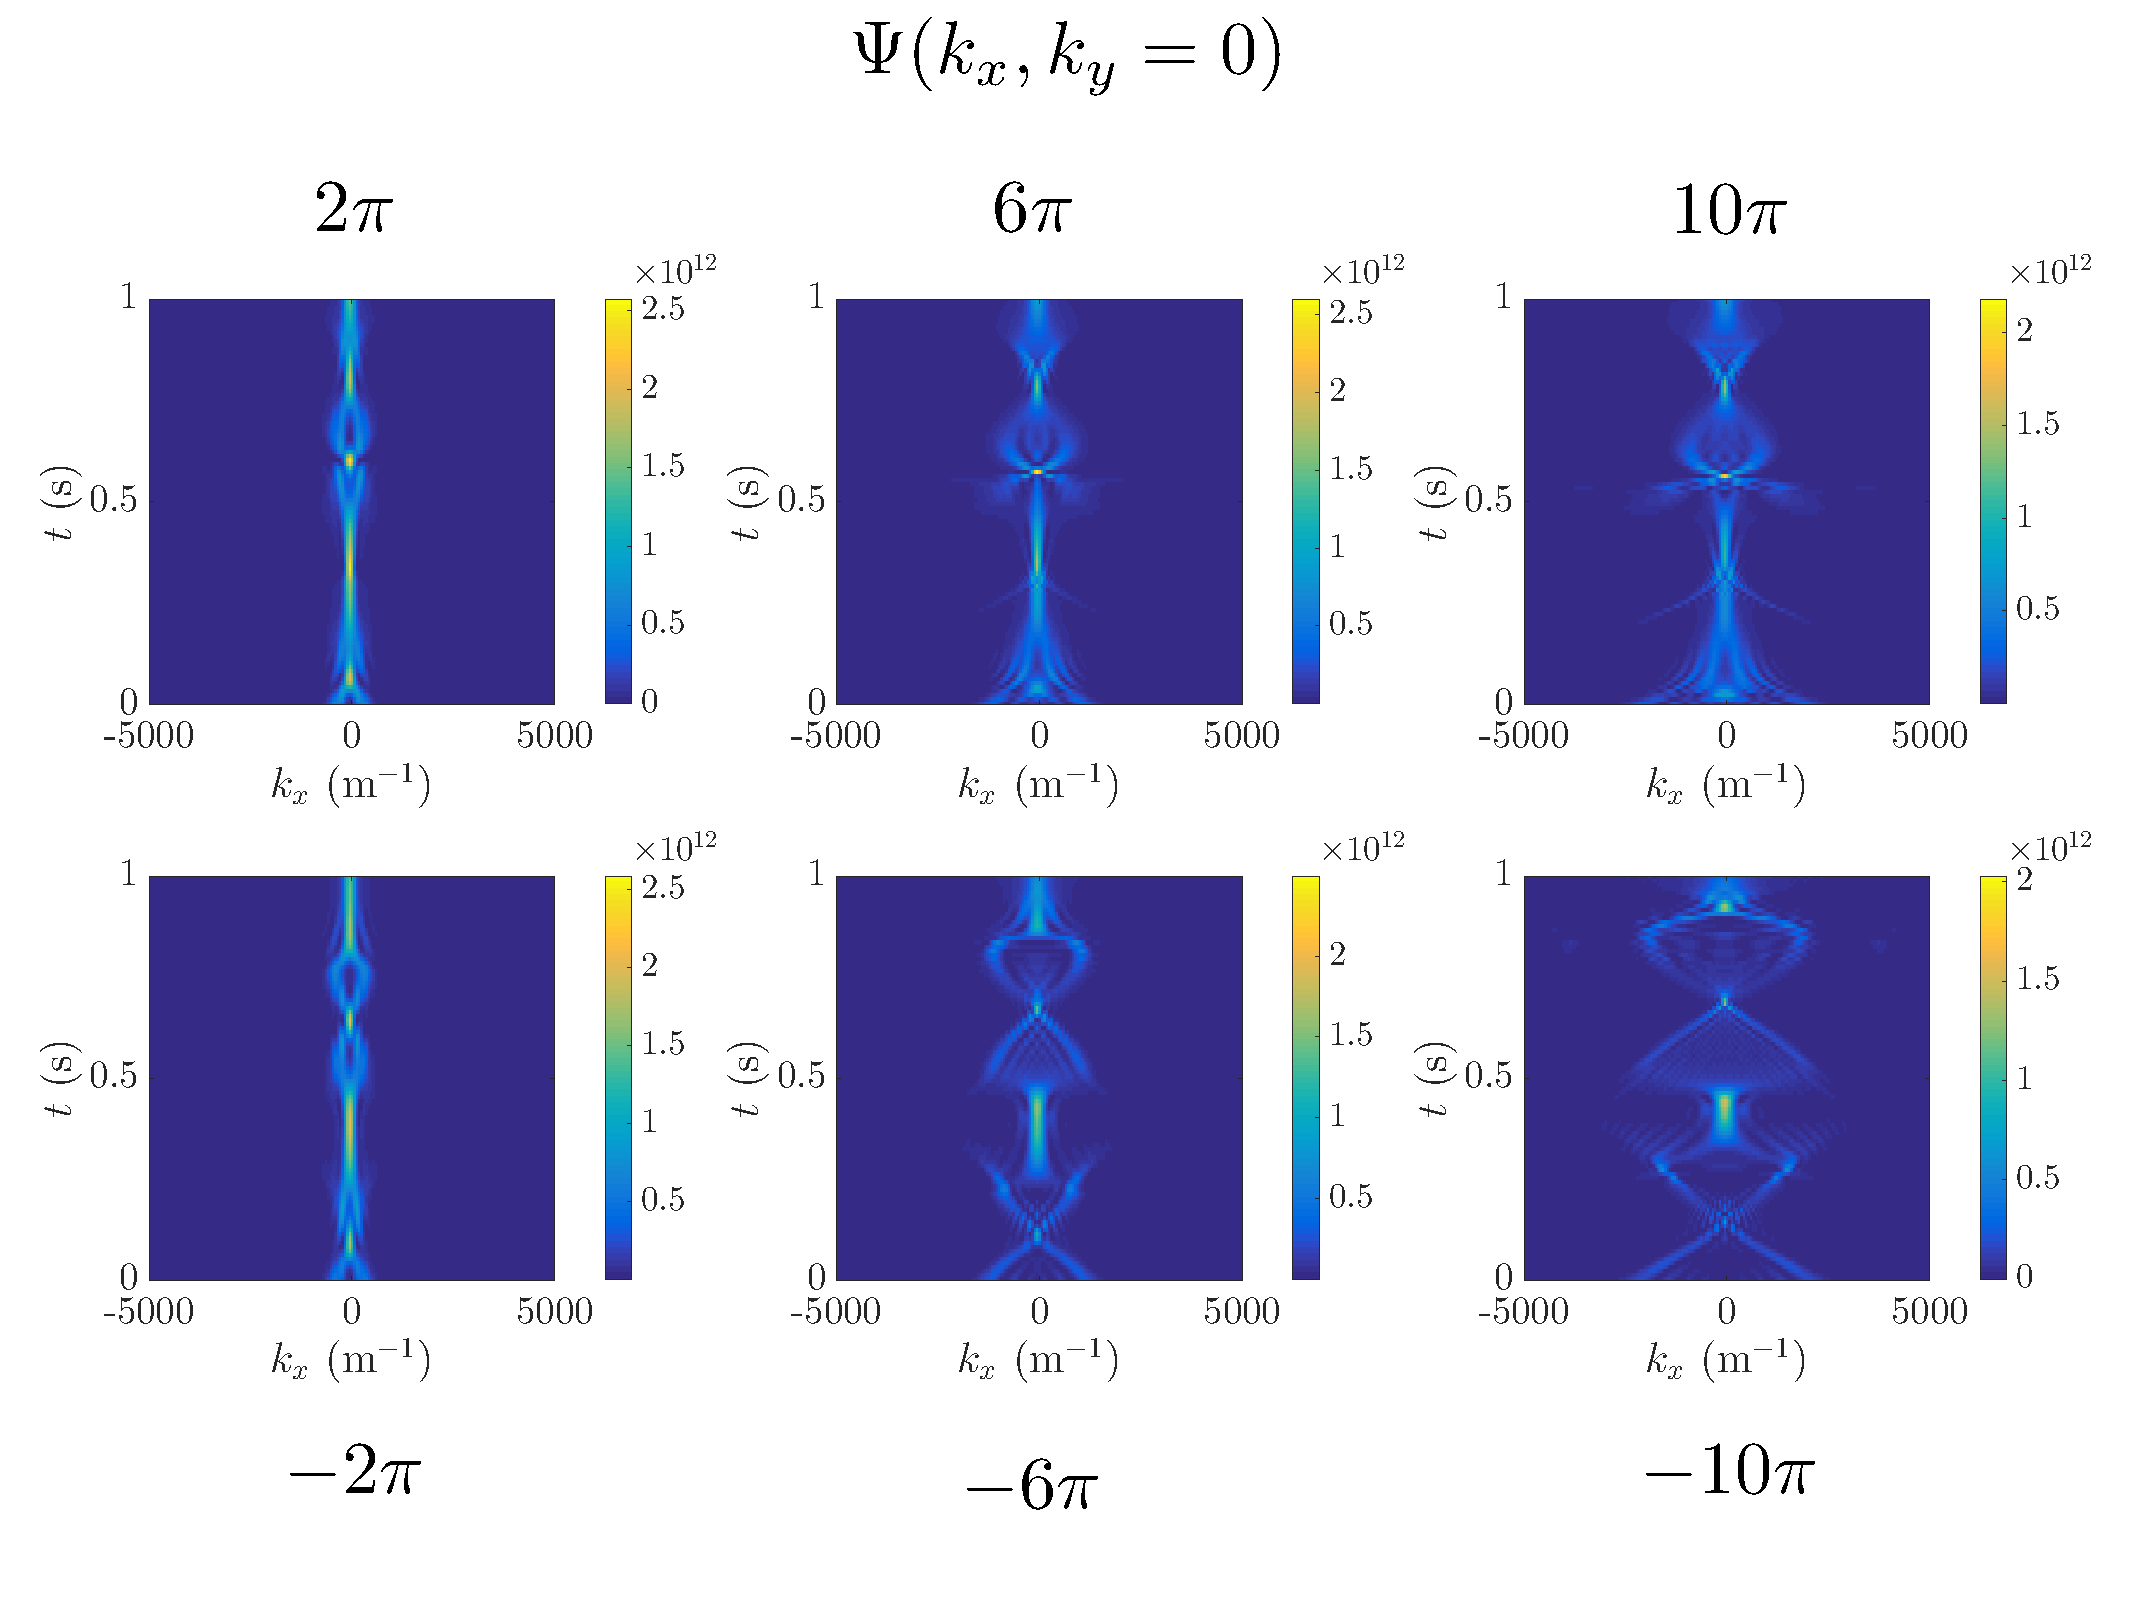
\includegraphics[width=0.95\textwidth]{Images/ch4_vtx/velocity/gaussian_imprint_wfck}
    \caption{A cut through the condensate wavefunction density following the phase imprinting of a Gaussian with amplitudes $A=\pm ( 2\pi, 6\pi, 10\pi)$. The positive imprints create an initial contraction of the cloud (top), while the negative imprints lead to expansion (bottom). For the larger kicking strengths interference fringes can be observed during expansion and contractions.}\label{fig:gaussian_wfc}
\end{figure}

%%%%%%%%%%%%%%%%%%%%%%%%%%%%%%%%%%%%%%%%%%%%%%%%%%%%%%%%%%%%
\section{Condensate analysis}\label{sec:con_analysis}
%%%%%%%%%%%%%%%%%%%%%%%%%%%%%%%%%%%%%%%%%%%%%%%%%%%%%%%%%%%%
To analyse the effects of the phase imprinting we will below introduce the decomposition of the kinetic energy to isolate the effect from phonons and vortices. Following this, for the vortex lattice we will introduce two closely linked methods to examine geometric structure - Delaunay triangulation and Voronoi tessellation. These methods are dual to one another, and can be used to easily identify order, structure and local parameters within systems of many particles.

\subsection{Kinetic energy decomposition}\label{sec:kinspec}
Given that the phase engineering modifies the condensate kinetic energy profile, it is instructive to quantify this effect. One can apply a spectral decomposition of the kinetic energy of the condensate into contributions solely from the vortices (incompressible), and those from the phonons (compressible)~\cite{CT:Nore_prl_1997,CT:Nore_pof_1997,CT:Bradley_prx_2012}. For this, the wavefunction is again written in terms of amplitude $\sqrt{\rho(\mathbf{r},t)}$ and phase $S(\mathbf{r},t)$, which allows the kinetic part of the Gross--Pitaevskii energy functional Eq.~\eqref{eqn:functional_full} to be calculated as
\begin{equation}
    E_{\text{kqp}} = \int d\mathbf{r} \left( \frac{\hbar^2}{2m}| \nabla\sqrt{\rho(\mathbf{r},t)} |^2  + \frac{m}{2}|\sqrt{\rho(\mathbf{r},t)}\mathbf{v}(\mathbf{r},t) |^2\right).
\end{equation}
One can then decompose this into the quantum pressure (first) and kinetic energy (second) terms. The kinetic energy term can be seen as a density-weighted velocity field, $\mathbf{u}(\mathbf{r},t) = \sqrt{\rho(\mathbf{r},t)}\mathbf{v}(\mathbf{r},t)$, and it can be further decomposed into the sum of compressible and incompressible terms,
\begin{equation}\label{eqn:kin_en}
    \mathbf{u(r},t) = \mathbf{u}^c(\mathbf{r},t) + \mathbf{u}^i(\mathbf{r},t).
\end{equation}
The two terms can be calculated by performing a Helmholtz decomposition of the field $\mathbf{u}$, which separates terms that are longitudinal ($\mathbf{u}^c$) and transversal ($\mathbf{u}^i$) with
\begin{subequations}\label{eqn:kinterms}
\begin{align}
    \nabla \times \mathbf{u}^c(\mathbf{r},t) &= 0, \\
    \nabla \cdot \mathbf{u}^i(\mathbf{r},t) &= 0.
\end{align}
\end{subequations}
By introducing the vector potential, $\mathbf{A}$, and the scalar potential, $B$, such that
\begin{subequations}
\begin{align}
    \mathbf{u}^c = \nabla B, \\
    \mathbf{u}^i = \nabla \times \mathbf{A},
\end{align}
\end{subequations}
we can rewrite Eq.~\eqref{eqn:kin_en} as
\begin{align}
    \nabla \times \mathbf{u}(\mathbf{r},t) = -\nabla^2 \mathbf{A}, \\
    \nabla \cdot \mathbf{u}(\mathbf{r},t) = \nabla^2 {B}.
\end{align}

To solve the above equation we begin by seeking a solution for $B$ by performing a spectral decomposition of the full density-weighted velocity field as
\begin{equation}
    B = \displaystyle\sum\limits_{j} \frac{k_j}{|\mathbf{k}|^2}\mathscr{F}[\mathbf{u}],
\end{equation}
where $k_j$ is the $j$-th component in $\mathbf{k}$ space, and $\mathscr{F}$ is the Fourier transform. The resulting solution for $\mathbf{u}^c$ is then given by
\begin{equation}
    \mathscr{F}[\mathbf{u}_i^c] = \displaystyle\sum\limits_{j} \frac{k_i k_j}{|\mathbf{k}|^2} \mathscr{F}[\mathbf{u}],
\end{equation}
which after taking note of Eq.~\eqref{eqn:kin_en} gives
\begin{align}
    \mathscr{F}[\mathbf{u}_i^i] &= \mathscr{F}[\mathbf{u}_i] - \mathscr{F}[\mathbf{u}_i^c]. \\
    &= \displaystyle\sum\limits_{j}\left(\delta_{i,j} - \frac{k_ik_j}{|\mathbf{k}|^2}\right)\mathscr{F}[\mathbf{u}_i]. \nonumber
\end{align}

This decomposition separates the energy contribution from phonons and vortex cores, represented by compressible and incompressible terms respectively~\cite{CT:Horng_pra_2009}. By averaging over binned shells in $\mathbf{k}$-space, the kinetic energy spectra, $E^{c,i}(k)$, are calculated as~\cite{CT:Bradley_prx_2012}
\begin{equation}\label{eqn:kin_spec_ic}
	E^{c,i}(k) = \frac{mk}{2}\sum\limits_{j\in\mathbf{r}} \int\limits_{0}^{2\pi}d\phi_k \frac{ |\mathcal{U}_j^{c,i}(\mathbf{k},t) |^2}{s_k},
\end{equation}
where
\begin{equation}
	\mathcal{U}_j^{c,i}(\mathbf{k},t) = \int d^2 \mathbf{r} e^{-\textrm{i}(\mathbf{k}\cdot\mathbf{r})} u_j^{c,i}(\mathbf{r},t).
\end{equation}
The terms $u_j^{c,i}(\mathbf{r},t)$ represent the position-space density-weighted velocity components in the specified shell, where $\phi_k$ is the polar angle, and $s_k$ is the number of values in the chosen shell.

%%%%%%%%%%%%%%%%%%%%%%%%%%%%%%%%%%%%%%%%%%%%%%%%%%%%%%%%%%%%
\subsection{Delaunay triangulation and Voronoi tessellation}\label{sec:delaunay}
%%%%%%%%%%%%%%%%%%%%%%%%%%%%%%%%%%%%%%%%%%%%%%%%%%%%%%%%%%%%
A common method for examining the ordering and periodicity of large-scale crystalline structures is to generate a mesh with each vertex being the location of a particle. With this, one can easily observe ordered and disordered regions in a material; well defined straight lines indicate a perfect crystal, with any bends indicating the presence of imperfections. Some of the most widely used methods for this are the dual techniques from computational geometry of Delaunay triangulation and Voronoi tessellation.

The Delaunay triangulation of an arbitrary set of points in Euclidian space, $\mathbf{R}$, which we will denote as $D(\mathbf{R})$, is constructed in the following way:
\begin{enumerate}
    \item No point will fall within the interior of any circumcircle of 3 points where $\mathbf{r}_{1..3} \subset \mathbf{R}$
    \item The Delaunay triangulation will maximise the minimum angle between points.
    \item If four points are on the same circumcircle, then both possible configurations give a Delaunay triangulation.
\end{enumerate}

\begin{figure}\centering
    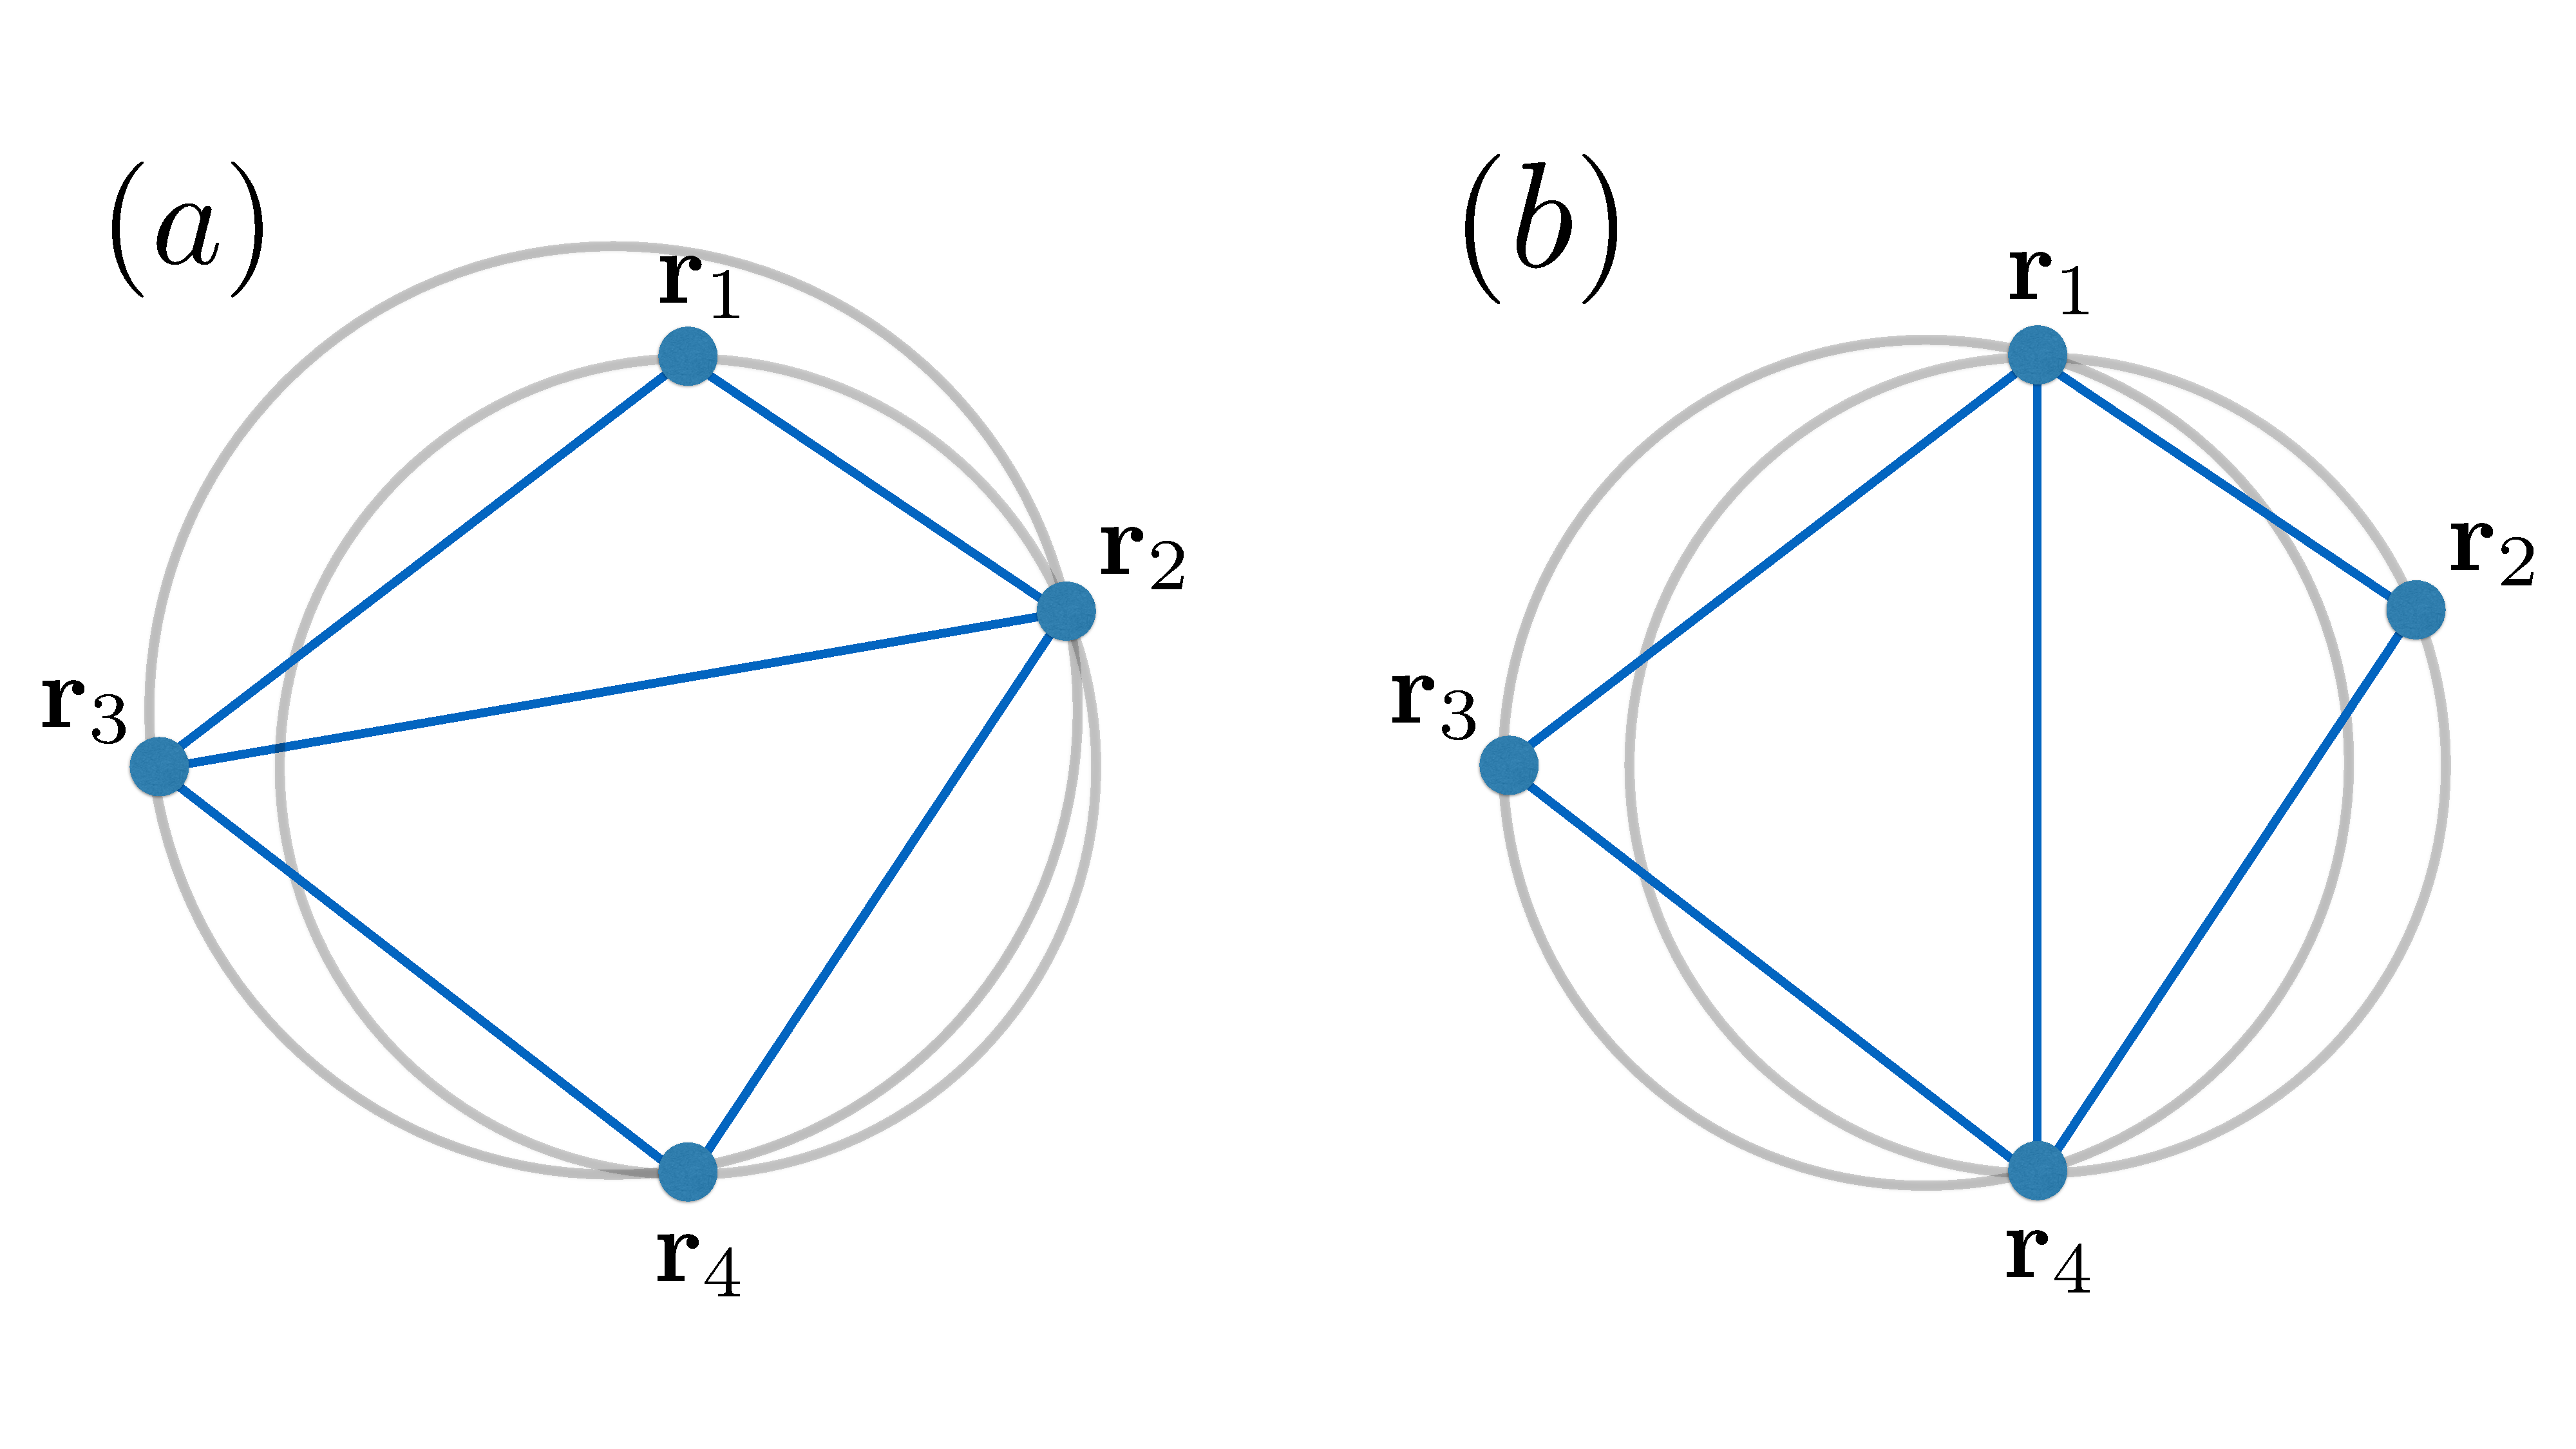
\includegraphics[width=0.45\textwidth]{Images/ch6_phasegineer/imgs/delaun}
    \caption{Non-Delaunay $(a)$ and Delaunay $(b)$ triangulation of 4 Euclidian points.}\label{fig:delaun}
\end{figure}
This concept is more easily explained visually. Fig.~\ref{fig:delaun} shows two different triangulations of four points; situation $(a)$ is a non-Delaunay triangulation, as the point $\mathbf{r}_1$ falls within the circumcircle of the other points. However, by simply flipping the central edge from $(\mathbf{r}_2, \mathbf{r}_3)$ to $(\mathbf{r}_1, \mathbf{r}_4)$ we can see in $(b)$ that we now have a valid Delaunay triangulation. No point falls within the circumcircle of the other points, and the minimum angle formed is maximised relative to configuration $(a)$. Following directly from this, one can see that Delaunay triangulation can be used to connect the closest vertices in a network. A nice side-effect of Delaunay triangulation is that one can examine when the number of edges from a vertex deviates from the expected value in the lattice, which is 6 for triangular lattices. This can be a useful means to locate defects in a crystal lattice, and we will make use of this during later discussions. This is performed using the built-in \textsc{MATLAB} function ``delaunayTriangulation'', and counting the number of attachments to each individual vertex. A triangulation of the vortex lattice from Fig.~\ref{fig:showingoff} within the previously discussed radial boundary of $r=2\times 10^{-4}$ m is shown in Fig.~\ref{fig:delaun_vtxlatt}.

\begin{figure}\centering
    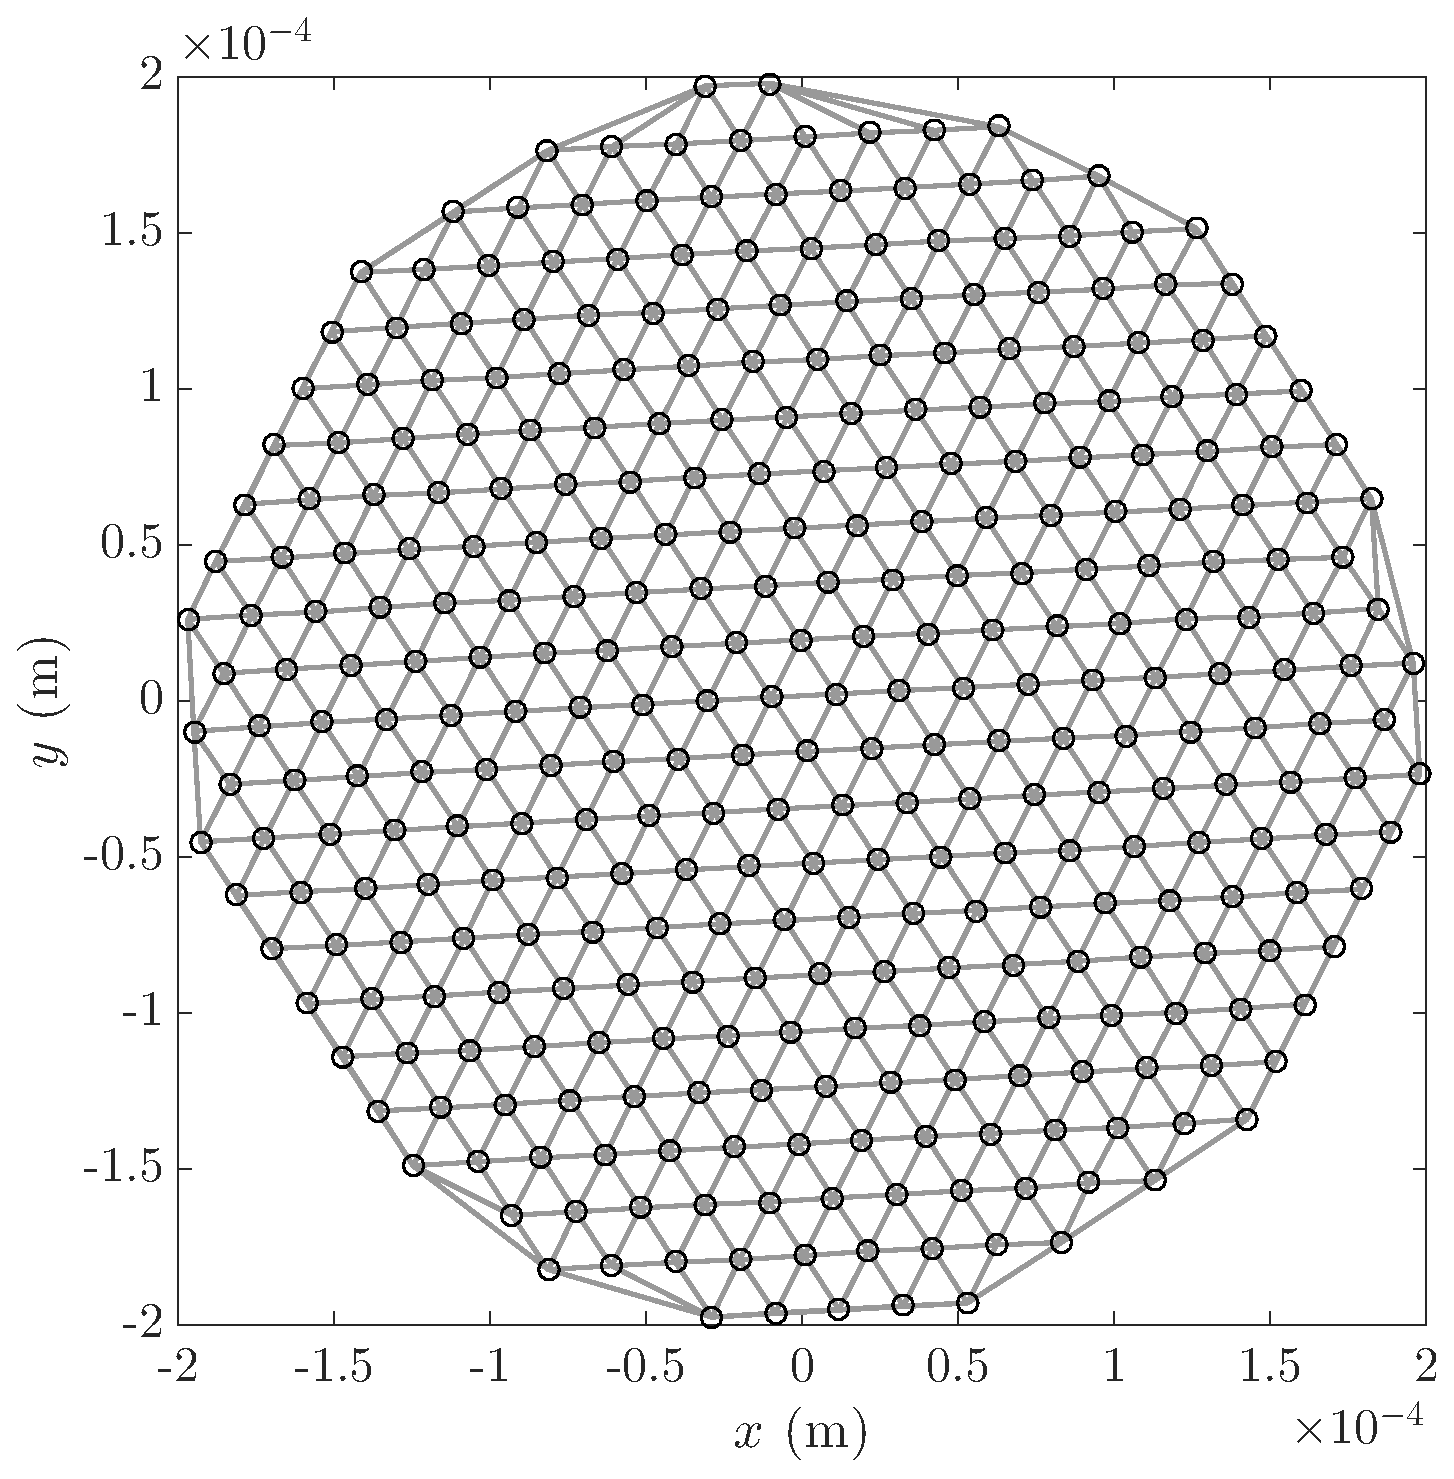
\includegraphics[width=0.45\textwidth]{Images/ch4_vtx/Del_tr_VTXLATT}
    \caption{Delaunay triangulation of the vortex lattice groundstate. The vertices away from the condensate boundary have the expected 6-edge structure.}\label{fig:delaun_vtxlatt}
\end{figure}

An alternative representation, using the dual of the Delaunay triangulation, is that of the Voronoi tessellation (diagram). The characteristic of these diagrams is that they are composed of cells each encompassing an individual vertex, within which all enclosed points are closer to that particular vertex than any other. This representation can be generated from the Delaunay triangulation and vice-versa. Taking the centres of the circumcircles describing the Delaunay triangulations, and connecting these forms the boundaries of the Voronoi cells. A simple generation method can be seen as creating and expanding the radius of circles (or $n$-spheres in $n$-dimensions) centred on each vertex. Where the circles intersect with one another defines the boundary of each individual cell. An example of a Voronoi diagram compared with a Delaunay triangulation is given by Fig.~\ref{fig:Voronoi}.
\begin{figure}\centering
    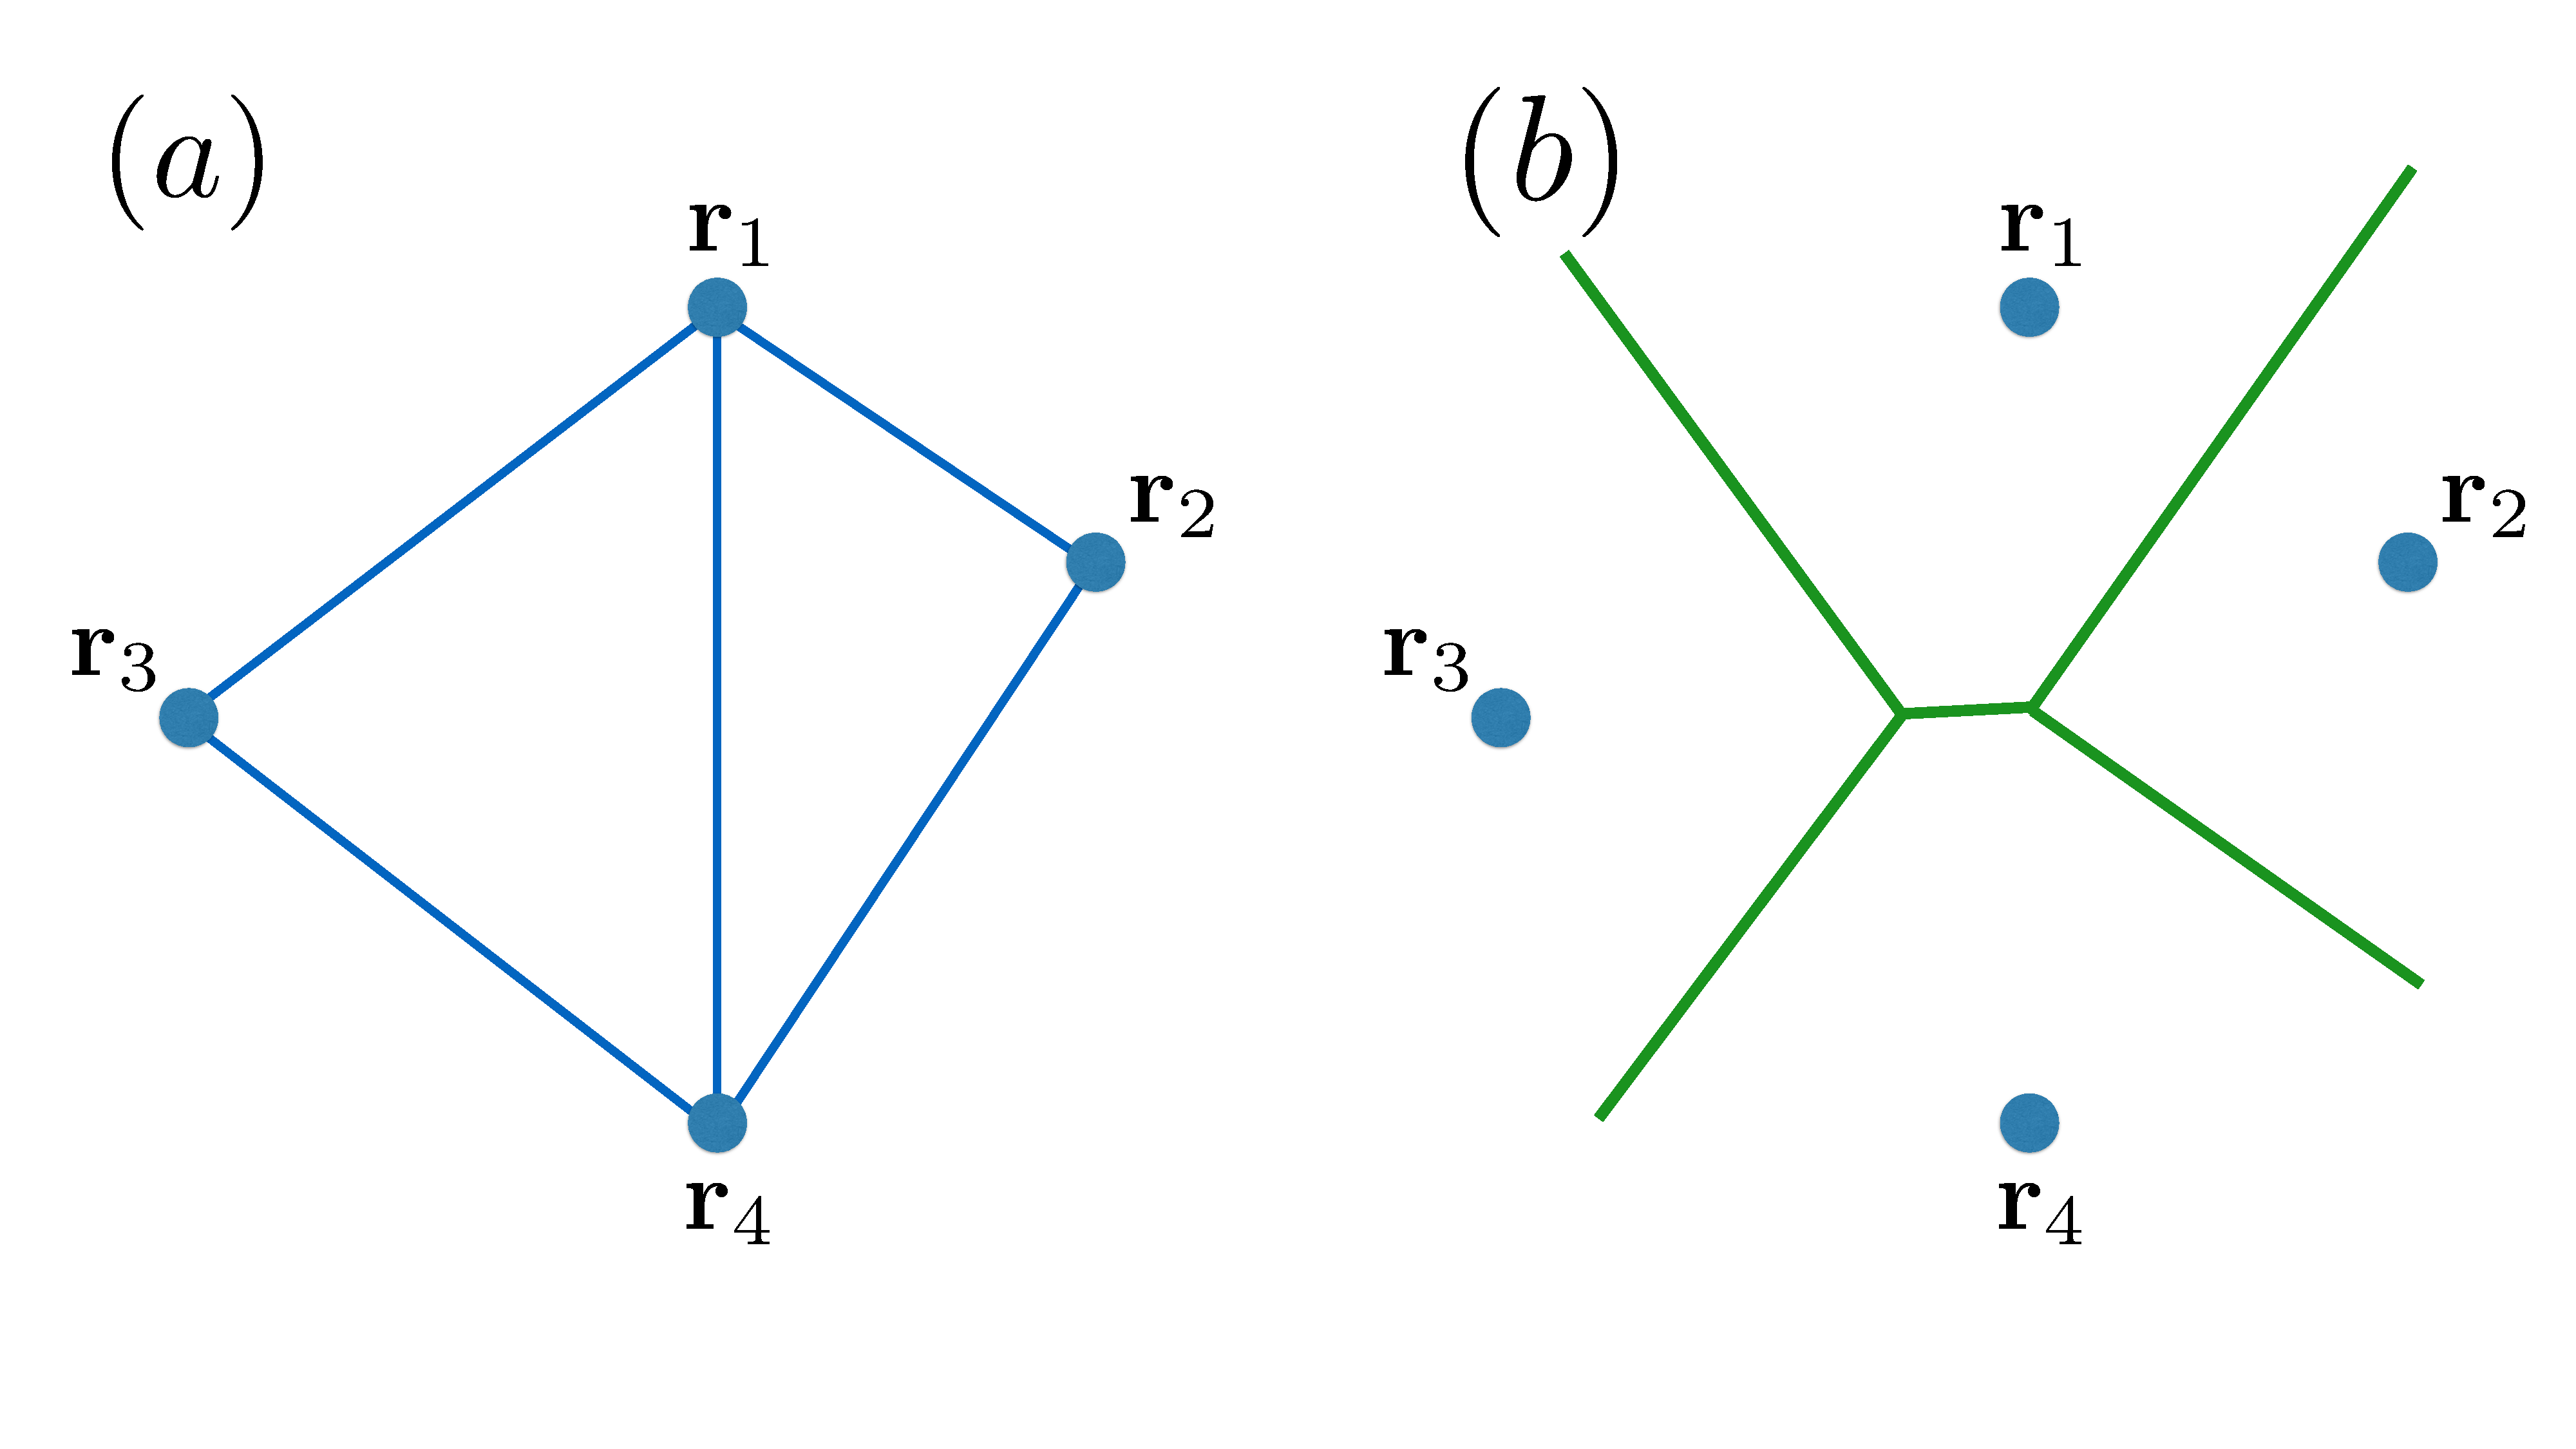
\includegraphics[width=0.55\textwidth]{Images/ch6_phasegineer/imgs/voronoi}
    \caption{Comparison of Delaunay triangulation $(a)$ with a Voronoi diamgram $(b)$. These graphs are duals, which means that one can be used to generate the other.}\label{fig:Voronoi}
\end{figure}
The area of each cell can be used as a metric of the strength of the interaction between particles in a many-body system, but also we may represent quantities local to each region in a system by the colour-scale of each cell. For the vortex lattice as given by Fig.~\ref{fig:showingoff}, a sample Voronoi diagram is given in Fig.~\ref{fig:voron_vtxlatt} with the color representing the area spanned by each Voronoi cell of the lattice.

\begin{figure}\centering
    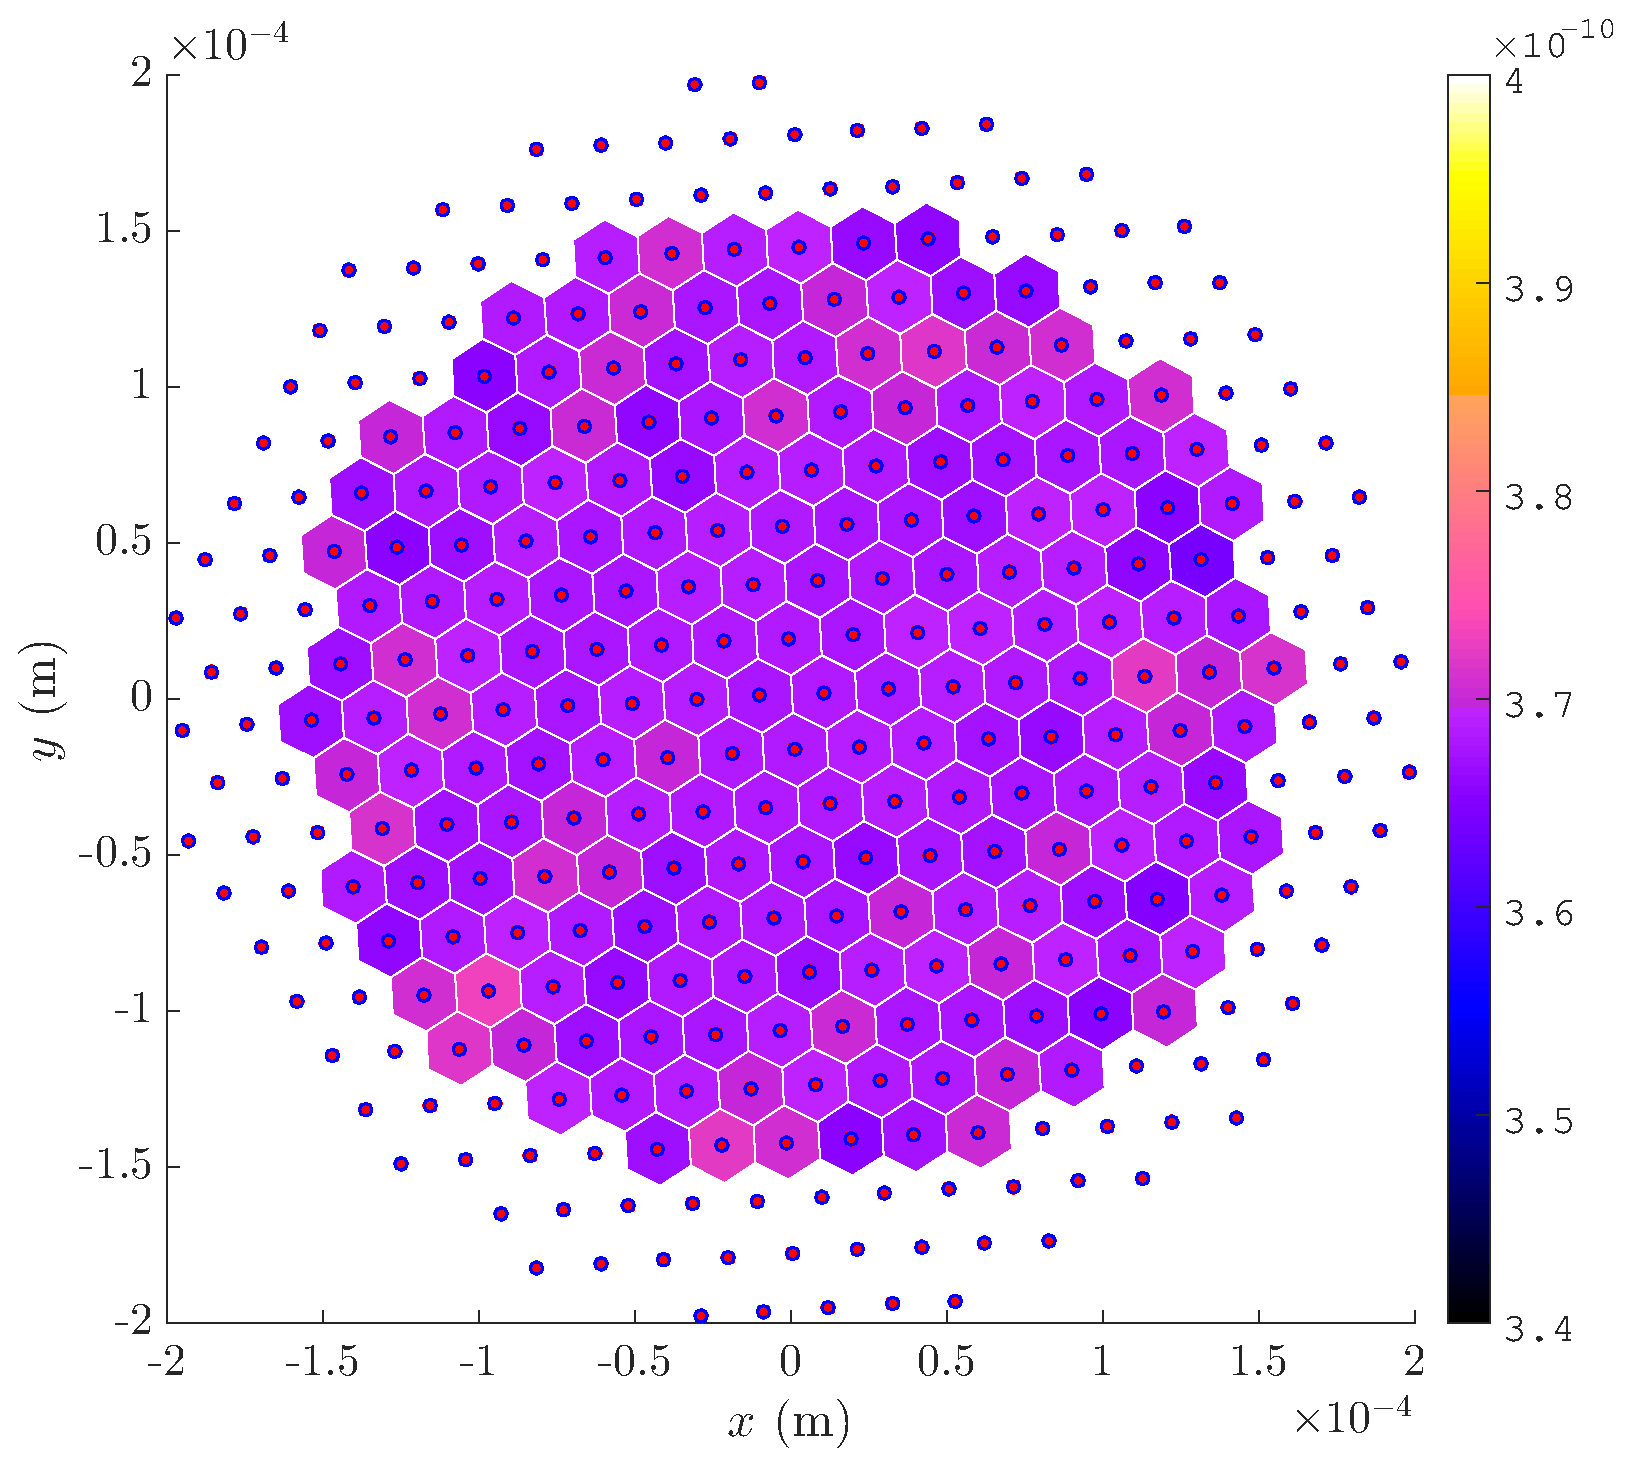
\includegraphics[width=0.55\textwidth]{Images/ch4_vtx/Voronoi_area_VTXLATT}
    \caption{Voronoi tesselation of the vortex lattice. The area of each cell is represented by the color mapping. To avoid the tessellation tending to infinity, a buffer region of vortices is created close to the boundary. }\label{fig:voron_vtxlatt}
\end{figure}
